%%%%%%%%%%%%%%%%%%%%%%%%%%%%%%%%%%%%%%%%%%%%%%%%%%%%%%%%%%%%%%%%%%%%%%%%%%%%%%%
%                       CARREGA DE LA CLASSE DE DOCUMENT                      %
%                                                                             %
% Les opcions admissibles son:                                                %
%      12pt / 11pt            (cos dels tipus de lletra; no feu servir 10pt)  %
%                                                                             %
% catalan/spanish/english     (llengua principal del treball)                 %
%                                                                             % 
% french/italian/german...    (si necessiteu fer servir alguna altra llengua) %
%                                                                             %
% listoffigures               (El document inclou un Index de figures)        %
% listoftables                (El document inclou un Index de taules)         %
% listofquadres               (El document inclou un Index de quadres)        %
% listofalgorithms            (El document inclou un Index d'algorismes)      %
%                                                                             %
%%%%%%%%%%%%%%%%%%%%%%%%%%%%%%%%%%%%%%%%%%%%%%%%%%%%%%%%%%%%%%%%%%%%%%%%%%%%%%%

\documentclass[11pt,spanish,listoffigures,listoftables]{tfgetsinf}

%%%%%%%%%%%%%%%%%%%%%%%%%%%%%%%%%%%%%%%%%%%%%%%%%%%%%%%%%%%%%%%%%%%%%%%%%%%%%%%
%                     CODIFICACIO DEL FITXER FONT                             %
%                                                                             %
%    windows fa servir normalment 'ansinew'                                   %
%    amb linux es possible que siga 'latin1' o 'latin9'                       %
%    Pero el mes recomanable es fer servir utf8 (unicode 8)                   %
%                                          (si el vostre editor ho permet)    % 
%%%%%%%%%%%%%%%%%%%%%%%%%%%%%%%%%%%%%%%%%%%%%%%%%%%%%%%%%%%%%%%%%%%%%%%%%%%%%%%

\usepackage[T1]{fontenc}
\usepackage[utf8]{inputenc} 
\usepackage{graphicx}
\usepackage{float}
\usepackage{adjustbox}
\usepackage{textcomp}   % Maneja comillas
\usepackage{lmodern}    % Fuente moderna
\usepackage{listings}   % Para mostrar código (opcional)
\usepackage{amsmath}    % Por si hay matemáticas
\usepackage[printonlyused]{acronym}





%%%%%%%%%%%%%%%%%%%%%%%%%%%%%%%%%%%%%%%%%%%%%%%%%%%%%%%%%%%%%%%%%%%%%
% Para conseguir que la tabla de contenido no salga en rojo
%%%%%%%%%%%%%%%%%%%%%%%%%%%%%%%%%%%%%%%%%%%%%%%%%%%%%%%%%%%%%%%%%%%%%

\hypersetup{ colorlinks=true, linkcolor=black, urlcolor=cyan, }

%%%%%%%%%%%%%%%%%%%%%%%%%%%%%%%%%%%%%%%%%%%%%%%%%%%%%%%%%%%%%%%%%%%%%%%%%%%%%%%
%                        ALTRES PAQUETS I DEFINICIONS                         %
%                                                                             %
% Carregueu aci els paquets que necessiteu i declareu les comandes i entorns  %
%                                          (aquesta seccio pot ser buida)     %
%%%%%%%%%%%%%%%%%%%%%%%%%%%%%%%%%%%%%%%%%%%%%%%%%%%%%%%%%%%%%%%%%%%%%%%%%%%%%%%



%%%%%%%%%%%%%%%%%%%%%%%%%%%%%%%%%%%%%%%%%%%%%%%%%%%%%%%%%%%%%%%%%%%%%%%%%%%%%%%
%                        DADES DEL TREBALL                                    %
%                                                                             %
% titol, alumne, tutor i curs academic                                        %
%%%%%%%%%%%%%%%%%%%%%%%%%%%%%%%%%%%%%%%%%%%%%%%%%%%%%%%%%%%%%%%%%%%%%%%%%%%%%%%

\title{Diseño e implementación de herramientas de análisis de genoma basadas en la Teoría de la Información}
\author{Cristina Rodríguez Fernández}
\tutor{Jose María Sempere Luna}
\curs{2024-2025}

%%%%%%%%%%%%%%%%%%%%%%%%%%%%%%%%%%%%%%%%%%%%%%%%%%%%%%%%%%%%%%%%%%%%%%%%%%%%%%%
%                     PARAULES CLAU/PALABRAS CLAVE/KEY WORDS                  %
%                                                                             %
% Independentment de la llengua del treball, s'hi han d'incloure              %
% les paraules clau i el resum en els tres idiomes                            %
%%%%%%%%%%%%%%%%%%%%%%%%%%%%%%%%%%%%%%%%%%%%%%%%%%%%%%%%%%%%%%%%%%%%%%%%%%%%%%%

\keywords{retinosi pigmentària, anàlisi genòmic, teoria de la informació, fonts de Markov, entropia, variants genètiques, visualització de dades, fitxer VCF, k-mers, densitat de mutacions}             % Paraules clau
         {retinosis pigmentaria, análisis genómico, teoría de la información, fuentes de Markov, entropía, variantes genéticas, visualización de datos, archivo VCF, k-mers, densidad de mutaciones}     % Palabras clave  
         {retinitis pigmentosa, genomic analysis, information theory, Markov sources, entropy, genetic variants, data visualization, VCF file, k-mers, mutation density}                                 % Key words

%%%%%%%%%%%%%%%%%%%%%%%%%%%%%%%%%%%%%%%%%%%%%%%%%%%%%%%%%%%%%%%%%%%%%%%%%%%%%%%
%                              INICI DEL DOCUMENT                             %
%%%%%%%%%%%%%%%%%%%%%%%%%%%%%%%%%%%%%%%%%%%%%%%%%%%%%%%%%%%%%%%%%%%%%%%%%%%%%%%

\begin{document}

%%%%%%%%%%%%%%%%%%%%%%%%%%%%%%%%%%%%%%%%%%%%%%%%%%%%%%%%%%%%%%%%%%%%%%%%%%%%%%%
%              RESUMEN DEL TFG EN CASTELLANO, VALENCIA I ANGLES                %
%%%%%%%%%%%%%%%%%%%%%%%%%%%%%%%%%%%%%%%%%%%%%%%%%%%%%%%%%%%%%%%%%%%%%%%%%%%%%%%

\begin{abstract}[spanish]
   Este Trabajo de Fin de Grado se ha centrado en el desarrollo de una herramienta computacional de análisis de secuencias genómicas basada en la Teoría de la Información, con el objetivo de estudiar cómo afectan ciertas mutaciones genéticas asociadas a enfermedades raras, en concreto la retinosis pigmentaria (RP). Para ello se han aplicado técnicas como el cálculo de entropía (tanto simple como condicional), el análisis de densidad de mutaciones a lo largo del genoma y el modelado de fuentes de Markov. 

   El sistema ha sido diseñado con un enfoque modular, separando la lógica del análisis de la parte visual mediante una interfaz gráfica. Esta interfaz permite la carga de archivos genómicos, la configuración de parámetros clave para el análisis (tamaño de k-mer, orden de fuente de Markov, tamaño de ventana...), y la visualización clara de los resultados. De esta manera, se facilita su uso para personal clínico o investigador que no tiene por qué contar con conocimientos avanzados de programación. 

   A partir de los archivos con las secuencias de referencia obtenidos del National Center for Biotechnology Information (NCBI) y archivos Variant Call Format (VCF) con mutaciones proporcionados por el IIS La Fe, esta herramienta es capaz de aplicar las mutaciones sobre la secuencia, construir fuentes de Markov y comparar las diferencias entre la versión original y la mutada. Los resultados muestran una alta correspondencia entre zonas con mayor densidad de mutaciones y valores anómalos de entropía, lo que podría ayudar a identificar zonas del genoma especialmente relevantes desde el punto de vista clínico. 

   Este sistema no solo permite automatizar el análisis de grandes volúmenes de datos genéticos, sino que podría ser base para futuros proyectos y su incorporación al ámbito médico en contextos reales. 
   \\
   \\
\end{abstract}
\begin{abstract}[catalan]

   Aquest Treball de Fi de Grau s'ha centrat en el desenvolupament d'una eina computacional per a l'anàlisi de seqüències genòmiques basada en la Teoria de la Informació, amb l'objectiu d'estudiar com afecten certes mutacions genètiques associades a malalties rares, concretament la retinosi pigmentària (RP). Per a això, s'han aplicat tècniques com el càlcul de l'entropia (tant simple com condicional), l'anàlisi de la densitat de mutacions al llarg del genoma i el modelatge de fonts de Markov. 

   El sistema ha sigut dissenyat amb un enfocament modular, separant la lògica de l'anàlisi de la part visual mitjançant una interfície gràfica. Aquesta interfície permet carregar fitxers genòmics, configurar paràmetres clau per a l'anàlisi (com la mida del k-mer, l'ordre de la font de Markov, o la mida de la finestra), i visualitzar els resultats de manera clara. Així es facilita el seu ús per a personal clínic o investigador que no tinga coneixements avançats en programació. 

   A partir dels fitxers amb les seqüències de referència obtingudes del National Center for Biotechnology Information (NCBI) i dels fitxers Variant Call Format (VCF) amb mutacions proporcionats per l'IIS La Fe, aquesta eina és capaç d'aplicar les mutacions sobre la seqüència, construir fonts de Markov i comparar les diferències entre la versió original i la mutada. Els resultats mostren una alta correspondència entre zones amb major densitat de mutacions i valors anòmals d'entropia, la qual cosa podria ajudar a identificar àrees del genoma especialment rellevants des del punt de vista clínic. 

   Aquest sistema no sols permet automatitzar l'anàlisi de grans volums de dades genètiques, sinó que també podria servir com a base per a futurs projectes i la seua integració en l'àmbit mèdic en contextos reals. 
   \\
   \\
\end{abstract}
\begin{abstract}[english]
   This Final Degree Project has focused on the development of a computational tool for genomic sequence analysis based on Information Theory, with the aim of studying how certain genetic mutations associated with rare diseases, specifically retinitis pigmentosa (RP), affect the genome. To achieve this, techniques such as entropy calculation (both simple and conditional), mutation density analysis across the genome have been applied and and Markov source modeling. 

   The system has been designed with a modular approach, separating the analysis logic from the visual layer using a graphical interface. This interface allows users to load genomic files, configure key analysis parameters (such as k-mer size, Markov model order, window size...), and clearly visualize the results. In doing so, it makes the tool accessible to clinical or research personnel without advanced programming knowledge. 

   Using reference sequence files from the National Center for Biotechnology Information (NCBI) and Variant Call Format (VCF) files with mutations provided by the IIS La Fe, the tool can apply the mutations to the sequence, build Markov sources, and compare the differences between the original and mutated versions. The results show a high correlation between regions with higher mutation density and abnormal entropy values, which could help identify clinically relevant areas of the genome. 

   This system not only enables the automation of large-scale genetic data analysis, but it could also serve as the foundation for future projects and its incorporation into real-world medical contexts. 
   \\
   \\
\end{abstract}

%%%%%%%%%%%%%%%%%%%%%%%%%%%%%%%%%%%%%%%%%%%%%%%%%%%%%%%%%%%%%%%%%%%%%%%%%%%%%%%
%                              CONTINGUT DEL TREBALL                          %
%%%%%%%%%%%%%%%%%%%%%%%%%%%%%%%%%%%%%%%%%%%%%%%%%%%%%%%%%%%%%%%%%%%%%%%%%%%%%%%

\mainmatter


%%%%%%%%%%%%%%%%%%%%%%%%%%%%%%%%%%%%%%%%%%%%%%%%%%%%%%%%%%%%%%%%%%%%%%%%%%%%%%%
%                                 ABREVIACIONES                               %
%%%%%%%%%%%%%%%%%%%%%%%%%%%%%%%%%%%%%%%%%%%%%%%%%%%%%%%%%%%%%%%%%%%%%%%%%%%%%%%

\chapter*{Lista de abreviaturas}
\addcontentsline{toc}{chapter}{Lista de abreviaturas}

\begin{acronym}[LOPDGDD] % La longitud de la abreviatura más larga para alinear
  \acro{ODS}{Objetivos de Desarrollo Sostenible}
  \acro{TFG}{Trabajo de Fin de Grado}
  \acro{IA}{Inteligencia Artificial}
  \acro{IIS}{Instituto de Investigación Sanitaria}
  \acro{RP}{Retinosis Pigmentaria}
  \acro{DHR}{Distrofias Hereditarias de Retina}
  \acro{DGR}{Distròfies Hereditàries de Retina}
  \acro{HRD}{Hereditary Retinal Dystrophies}
  \acro{ML}{Machine Learning}
  \acro{VCF}{Variant Call Format}
  \acro{FASTA}{Fast-All (formato de secuencia biológica)}
  \acro{SNP}{Single Nucleotide Polymorphism}
  \acro{ADN}{Ácido Desoxirribonucleico}
  \acro{ARN}{Ácido Ribonucleico}
  \acro{INDEL}{Inserción o Deleción de nucleótidos}
  \acro{WES}{Whole Exome Sequencing}
  \acro{NGS}{Next Generation Sequencing}
  \acro{CNV}{Copy Number Variation}
  \acro{SV}{Structural Variation}
  \acro{NCBI}{National Center for Biotechnology Information}
  \acro{TFM}{Trabajo de Fin de Máster}
  \acro{CNN}{Convolutional Neural Network}
  \acro{RGPD}{Reglamento General de Protección de Datos}
  \acro{LOPDGDD}{Ley Orgánica 3/2018 de Protección de Datos Personales y Garantía de los Derechos Digitales}
  \acro{UPV}{Universitat Politècnica de València}
\end{acronym}

%%%%%%%%%%%%%%%%%%%%%%%%%%%%%%%%%%%%%%%%%%%%%%%%%%%%%%%%%%%%%%%%%%%%%%%%%%%%%%%
%                                 INTRODUCCION                                %
%%%%%%%%%%%%%%%%%%%%%%%%%%%%%%%%%%%%%%%%%%%%%%%%%%%%%%%%%%%%%%%%%%%%%%%%%%%%%%%

\chapter{Introducción}

La retinosis o retinitis pigmentaria (\acs{RP}), una de las distrofias hereditarias de retina (\acs{DHR}) más frecuente, es un grupo de enfermedades conocidas por una degradación progresiva en los fotorreceptores que termina por causar pérdida visual irreversible. Esta patología suele manifestarse en un principio con ceguera nocturna, seguida por una reducción del campo visual periférico y, en fases avanzadas, puede llegar a la pérdida de la visión central\cite{NAT}. Aún con los recientes avances en la secuenciación del genoma humano, el origen de esta condición sigue siendo un desafío debido a la amplia diversidad genética involucrada y la cantidad de genes relacionados con las \acs{DHR}. 

\begin{figure}[H]
   \centering
   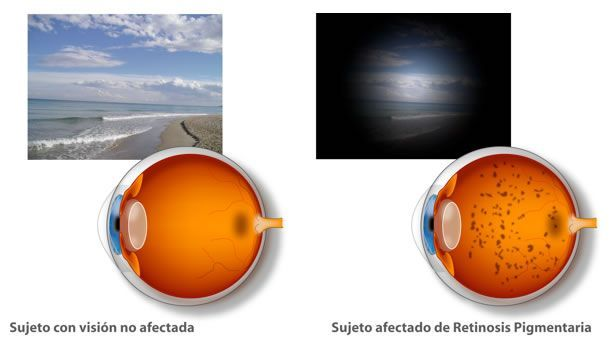
\includegraphics[width=0.9\textwidth]{Retinosis-Pigmetaria.jpg}
   \caption{Ejemplo de visión de un paciente con visión normal y un paciente con \acs{RP}.}
   \label{fig:etiqueta_opcional2}
\end{figure}

Este Trabajo de Fin de Grado, continuación del Trabajo de Fin de Máster (\acs{TFM}) de Andrea Vañó Ribelles\cite{VAN} y el Trabajo de Fin de Grado de Luis Alberto Martínez Bravo\cite{MAR}, explora el uso de herramientas de Teoría de la Información y modelos de fuentes de Markov para analizar el genoma humano, con el objetivo de predecir posibles mutaciones asociadas a la \acs{RP}. Puesto que la \acs{RP} es una enfermedad rara y el número de personas afectadas es muy pequeño, las técnicas de Machine Learning (\acs{ML}) no resultan lo suficientemente efectivas debido a la falta de datos para desarrollar modelos robustos. 

 

En vez de ello, este enfoque se centra en el análisis de regiones genómicas con elevada entropía y densidad de mutaciones, ya que estas áreas serían clave para detectar variantes con mayor probabilidad de estar vinculadas a la enfermedad. 

 

Para ello, se han empleado los datos genómicos del National Center for Biotechnology Information (\acs{NCBI}) y archivos \acs{VCF} proporcionados por el Grupo de Investigación de Biomedicina Molecular, Celular y Genómica del \acs{IIS} La Fe. El propósito del estudio es profundizar en las características del genoma asociadas a la enfermedad y aportar nuevas maneras de optimizar el diagnóstico genético de la retinosis pigmentaria. 

\section{Contexto}

Se conoce como “enfermedad rara” o “huérfana” a aquellas enfermedades que afectan a un bajo número de personas, es decir, que tienen una baja incidencia. En Europa el rango para considerar a una enfermedad como rara se sitúa en 5 personas afectadas por cada 10.000, mientras que en Estados Unidos se considera rara cuando afecta a menos de 200.000 personas\cite{ENF}.

Sin embargo, son muchas las personas que conviven con ellas, más de 300 millones en el mundo, 3 de ellos en España, ya que se estima que existen más de 7.000 enfermedades raras, de las cuales se han identificado 6.417 según datos recientes\cite{CON}.

Estas patologías suelen ser crónicas, progresivas, tienen origen genético y, con frecuencia son de carácter invalidante. Además, pueden afectar tanto a las capacidades físicas de las personas como a las mentales, conductuales y sensoriales. Normalmente comienzan a manifestarse de forma temprana, se estima que hasta en dos tercios de los pacientes los síntomas comienzan antes de los 2 años, aunque pueden aparecer a lo largo de toda la vida. 

La retinosis pigmentaria (\acs{RP}) es un conjunto de enfermedades hereditarias degenerativas que afectan a la retina, provocando una pérdida progresiva de la visión. La \acs{RP} es una de las Distrofias Hereditarias de Retina (\acs{DHR}) más comunes, pero existen otras como la enfermedad de Stargardt, la distrofia viteliforme de Best, y el síndrome de Usher. Como su nombre indica, esta enfermedad afecta directamente a la retina, es decir, la capa interna y posterior del ojo, sensible a la luz, donde se encuentra la mayor parte de los fotorreceptores. Estos fotorreceptores son células especializadas que convierten la luz en señales eléctricas, que luego se transmiten al cerebro a través del nervio óptico\cite{GAR}.

\begin{figure}[H]
   \centering
   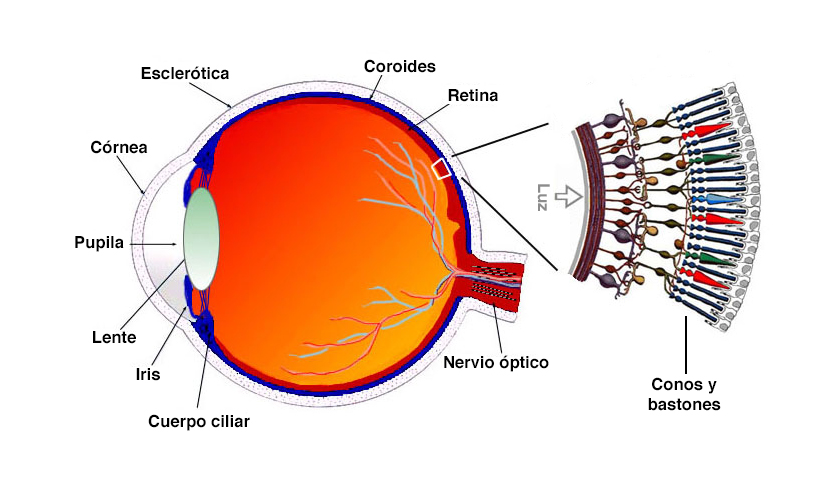
\includegraphics[width=0.9\textwidth]{retina.jpg}
   \caption{Esquema de las distintas partes del ojo.}
   \label{fig:etiqueta_opcional21}
\end{figure}

Existen dos tipos principales de fotorreceptores: 

\begin{itemize}
\item Bastones, que nos permiten ver en condiciones de poca luz y encargados de la visión nocturna y periférica. 
\item Conos, los cuales nos permiten distinguir colores y detalles cuando hay luz y responsables de la visión central. 
\end{itemize}

\begin{figure}[H]
   \centering
   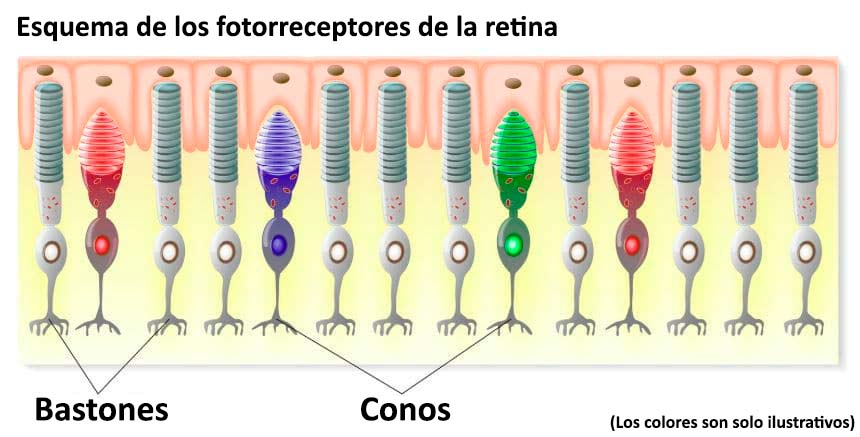
\includegraphics[width=0.9\textwidth]{fotorreceptores.jpg}
   \caption{Tipos de fotorreceptores.}
   \label{fig:etiqueta_opcional22}
\end{figure}

En las personas con \acs{RP}, los bastones son los primeros en deteriorarse, lo que explica que uno de los primeros síntomas sea la ceguera nocturna o dificultad para ver en la oscuridad. A medida que estos bastones se van dañando, también se reduce el campo visual o visión periférica. Los pacientes comienzan a experimentar lo que se conoce como “visión en túnel”.

Con el tiempo, la enfermedad también comienza a afectar a los conos. Cuando esto ocurre, la visión central comienza a deteriorarse, haciendo difíciles tareas cotidianas como leer, reconocer rostros o distinguir colores. Finalmente, en las etapas más avanzadas, la persona puede quedar prácticamente ciega. 

Este deterioro no ocurre de un día para otro, sino que se desarrolla progresivamente, y tanto su ritmo como los primeros síntomas pueden variar mucho de una persona a otra, aunque suelen empezar en la adolescencia o juventud y empeoran con los años. 

Esta enfermedad suele ser bilateral, simétrica y puede tener un patrón de herencia autosómico dominante, recesivo o ligado al cromosoma X, con más de 70 genes identificados hasta la fecha que podrían estar relacionados\cite{GIL}. El diagnóstico se basa en exámenes oftalmológicos como la oftalmoscopia, angiofluoresceinografía, campimetría, pruebas de agudeza visual, adaptación a la oscuridad y electrorretinograma, además de estudios genéticos\cite{VIS}.

Desde el punto de vista social, las personas con \acs{RP} deben enfrentar barreras significativas en su vida diaria, ya que muchas veces limita la movilidad, la autonomía en tareas domésticas y la participación en actividades sociales. La investigación revela que estas personas sufren exclusión social agravada por el ocularcentrismo, es decir, la estructura social en torno a la visión como sentido principal. Además, la falta de adaptaciones tecnológicas, el desconocimiento social y la carencia de servicios accesibles intensifican las dificultades emocionales, como el nerviosismo, la dependencia y la frustración\cite{DEL}.


\section{Motivación}

\subsection{Motivación personal}
Desde que comencé mi formación en Ingeniería Informática, siempre he tenido la convicción de que esta no debe limitarse a aspectos técnicos, algoritmos o eficiencia computacional, sino que debe orientarse también hacia herramientas que tengan un impacto positivo en la vida de las personas. Por eso, me interesan especialmente las aplicaciones la Inteligencia Artificial para mejorar la sociedad, hacer el mundo más justo e inclusivo y resolver problemas reales.  

Siguiendo estos objetivos, y gracias al proyecto conjunto del Instituto VRAIN con el Grupo de Investigación del \acs{IIS} La Fe de Biomedicina Molecular, Celular y Genómica, he tenido la oportunidad de formarme en diversas áreas y aplicar mis conocimientos técnicos a una dimensión ética y social. Por esta razón, considero que mejorar la calidad de vida de pacientes mediante herramientas que ayuden a investigadores y personal sanitario en el diagnóstico es una de las principales motivaciones que me impulsa en la realización de este proyecto. 

\subsection{Motivación profesional}
Las distrofias hereditarias de retina (\acs{DHR}) constituyen un conjunto de enfermedades genéticas que afectan a la estructura y función de la retina, llevando progresivamente a la pérdida de visión, en muchos casos hasta alcanzar la ceguera legal. A pesar de ser consideradas enfermedades raras, su impacto es profundo y duradero, no solo desde el punto de vista funcional, sino también psicológico, afectando significativamente la calidad de vida de quienes las padecen\cite{STO}.

Actualmente, no existe ningún tratamiento curativo, aunque se están explorando alternativas terapéuticas como las que se describen en la sección 2 de esta memoria, pero aún se encuentran en fase experimental. En este contexto, el diagnóstico genético tiene un papel fundamental en la orientación médica y la inclusión del paciente en ensayos clínicos\cite{HAN}.

Uno de los principales desafíos en el estudio genético de las distrofias hereditarias de retina (\acs{DHR}) radica en la gestión y análisis de la enorme cantidad de variantes obtenidas a partir de técnicas como la secuenciación del exoma completo (\acs{WES}). Aunque se aplican filtros por frecuencia poblacional o predictores del impacto funcional, el volumen de información sigue siendo elevado, lo que dificulta alcanzar un diagnóstico genético preciso\cite{DEC}.

En este trabajo se propone un enfoque complementario, basado en el uso de modelos computacionales que aplican principios de la Teoría de la Información para analizar la secuencia genómica antes y después de la introducción de mutaciones. A través de métricas como la entropía y la densidad mutacional, se busca detectar alteraciones estructurales o funcionales que puedan asociarse con variantes patológicas. Esta estrategia no solo contribuye al desarrollo de nuevas herramientas de apoyo al diagnóstico, sino que también tiene una dimensión humana relevante: mejorar el acceso a un diagnóstico certero, lo que representa un paso fundamental para que los pacientes y sus familias encuentren respuestas, orientación clínica y esperanza de acceso a futuras terapias. 

\section{Objetivos}

El objetivo principal de este Trabajo de Fin de Grado es proporcionar herramientas informáticas para el análisis genómico, en concreto aplicado a enfermedades raras como la retinosis pigmentaria (\acs{RP}). Para ello contamos con archivos que contienen información sobre mutaciones y secuencias completas del genoma, y se implementan modelos basados en Teoría de la Información y fuentes de Markov, con el fin de identificar regiones genómicas relevantes y predecir mutaciones potencialmente patogénicas.

\subsection{Procesamiento de archivos \acs{VCF} y secuencias genómicas}

Hacer uso de herramientas y librerías de uso biomédico que permitan la lectura, escritura y análisis de archivos genéticos, y de esta manera, realizar un preproceso y de la información genética y aplicar mutaciones sobre la secuencia de referencia de forma precisa y eficiente.

Preguntas de Investigación: 
\begin{itemize}
\item ¿Qué formato presentan los archivos \acs{VCF} y cómo se puede garantizar la compatibilidad con los archivos \acs{FASTA} con la secuencia genómica?
\item ¿Cómo se pueden integrar las trasformaciones necesarias en la secuencia de referencia de manera correcta y sin conflictos entre ellas?
\end{itemize}

\subsection{Aplicación de Teoría de la Información y fuentes de Markov al análisis de secuencias genómicas }

Utilizar modelos de Teoría de la Información y fuentes de Markov para predecir el impacto de las mutaciones en la secuencia genómica y así detectar zonas con valores anómalos de entropía, o alta densidad de mutaciones, para su posterior estudio. 

Preguntas de Investigación: 
\begin{itemize}
\item ¿Qué diferencias se observan en los valores de entropía, tanto la simple como la realizada a partir de aplicar fuentes de Markov, entre la secuencia original y la mutada? 
\item ¿Hay alguna correlación entre las zonas con alta densidad de mutaciones y los valores de entropía? 
\item ¿Cómo es la estructura que presentan las transiciones del modelo generado a partir de fuentes de Markov de orden k? 
\item ¿Cuáles son los valores óptimos de los parámetros para obtener resultados interesantes? 
\end{itemize}

\subsection{Desarrollo de una interfaz de usuario para la visualización de resultados }

Crear una aplicación para facilitar el uso del programa, sin necesidad de tener conocimientos avanzados en informática. Esto es especialmente importante en este contexto, ya que se trata de una herramienta enfocada a un usuario que no es experto en informática. Además, esta interfaz debe permitir la interacción del usuario con la aplicación, modificando distintos parámetros para obtener diferentes resultados en función de lo que se busque, y visualizar gráficamente y de manera unificada los resultados de este análisis. 

Preguntas de Investigación: 
\begin{itemize}
\item ¿Qué diseño debe tener la interfaz para que no sea demasiado compleja, pero permita interactuar ampliamente al usuario? 
\item ¿Cómo presentar los resultados de manera ordenada, clara y concisa, para hacer accesible la información más complicada? 
\end{itemize}

\subsection{Contribución a las aplicaciones de la \acs{IA} en el campo de la investigación genética }

Proponer un nuevo enfoque de análisis genómico basado en la Teoría de la Información, el cual no se había estudiado aún, y ofrecer una herramienta efectiva para el estudio de otras enfermedades raras con componente genético. 

Preguntas de Investigación: 
\begin{itemize}
\item ¿Debe poder generalizarse el proyecto para otras patologías? 
\item ¿Qué técnicas se podrían utilizar sobre los resultados obtenidos, como \acs{ML}, para clasificar o encontrar patrones de mutaciones? 
\end{itemize}


\section{Estructura de la memoria}

La memoria de este \acs{TFG} está estructurada en 7 secciones, cada una de estas a su vez divididas en subsecciones.  


La primera sección se introduce el proyecto, se exponen el contexto y la motivación, y se justifican los objetivos. En la sección 2, se realiza una investigación del conocimiento y tecnologías existentes en la actualidad sobre el tema que se aborda en el proyecto, así como las limitaciones que aún existen, lo que justifica la necesidad de este proyecto. En la sección 3, se realiza una exposición de los conceptos clave necesarios para entender este trabajo, genética y mutaciones, los archivos genómicos utilizados y los principios de la Teoría de la Información. Después, en la sección 4, se describe la metodología seguida y el flujo de información y herramientas usadas a lo largo del proyecto. En la sección 5, se explica detalladamente el funcionamiento del programa. En la sección 6 se exponen y analizan los resultados obtenidos mediante la realización de pruebas cambiando los diferentes parámetros. Por último, en la sección 7, se finaliza el trabajo, explicando las conclusiones obtenidas, seguida por un listado de las referencias bibliográficas utilizadas. 


%\section{Notes bibliografiques} %%%%% Opcional

%????? ????????????? ????????????? ????????????? ????????????? ?????????????

%%%%%%%%%%%%%%%%%%%%%%%%%%%%%%%%%%%%%%%%%%%%%%%%%%%%%%%%%%%%%%%%%%%%%%%%%%%%%%%
%                                ESTADO DEL ARTE                              %
%%%%%%%%%%%%%%%%%%%%%%%%%%%%%%%%%%%%%%%%%%%%%%%%%%%%%%%%%%%%%%%%%%%%%%%%%%%%%%%

\chapter{Estado del arte}

El campo del análisis genómico de la retinosis pigmentaria (\acs{RP}) está avanzando rápidamente, con desarrollos en la identificación genética, herramientas de predicción y terapias emergentes. Sin embargo, en un contexto de disponibilidad limitada de especialistas en retina, pruebas y asesoramiento genético, sigue existiendo una gran necesidad de métodos diagnósticos precisos y accesibles. Esta situación ha motivado la búsqueda de nuevas técnicas para mejorar la detección de esta enfermedad.

\section{Métodos tradicionales}

Los métodos tradicionales basados en sistemas de codificación médica como el ICD (International Classification of Diseases) y el SNOMED (Systematized Nomenclature of Medicine) han sido ampliamente utilizados en la medicina para clasificar enfermedades y registrar diagnósticos. Sin embargo, en el caso de enfermedades genéticas raras como la retinosis pigmentaria (\acs{RP}), estos sistemas de codificación presentan importantes limitaciones\cite{VER}. Esto es debido a que es una patología altamente heterogénea a nivel genético y clínico: existen numerosas mutaciones responsables y los síntomas pueden evolucionar de formas muy diversas entre pacientes\cite{HAR}. 

Debido a esta complejidad, se ha recurrido a técnicas más especificas como los paneles genéticos dirigidos o la secuenciación de exoma completo (\acs{WES}). Estos enfoques son capaces de examinar una gran cantidad de mutaciones de cada paciente. No obstante, muchos pacientes quedan sin un diagnositco definitivo debido a la dificultad para interpretar el gran volumen de información relativa a las variantes encontradas tras la secuenciación.

\section{Inteligencia Artificial}

En la actualidad se están utilizando métodos basados en Inteligencia Artificial (\acs{IA}) para la detección, diagnóstico y pronóstico de numerosas enfermedades en distintas áreas de la medicina, desde oncología hasta neurología o cardiología. Esto es debido a la capacidad de la \acs{IA} para trabajar con grandes volúmenes de datos e identificar en estos patrones complejos para generar predicciones con una alta precisión\cite{FER}. No obstante, su desarrollo para las distrofias hereditarias de retina (\acs{DHR}), específicamente la retinosis pigmentaria (\acs{RP}) todavía está en una fase temprana.

\subsection{Aplicaciones de Machine Learning}

El aprendizaje profundo (deep learning) es una subcategoría de la Inteligencia Artificial (\acs{IA}) que ha ganado mucha atención en los últimos años, especialmente porque el aprendizaje profundo es muy eficaz en el reconocimiento de patrones y el análisis de imágenes\cite{STE}.

Inspirado en el cerebro humano, el aprendizaje profundo (Deep Learning) ha sido desarrollado utilizando redes neuronales para aprender a partir de datos, extrayendo y comprendiendo automáticamente características complejas. Un ejemplo común del uso del aprendizaje profundo en imágenes médicas son las redes neuronales convolucionales (\acs{CNN}, por sus siglas en inglés). Las \acs{CNN} participan en diversas tareas relacionadas con imágenes, como la detección, el reconocimiento y la segmentación de imágenes, mediante el uso de información espacial, la detección de características locales y la reducción de la complejidad del modelo a través del muestreo, el uso compartido de pesos y los campos receptivos locales\cite{SHE}.

En un estudio reciente, se utilizaron tres modelos preentrenados; Inception-v3, ResNet-50 y VGG-19, para clasificar imágenes retinianas asociadas a diferentes genes relacionados con la retinosis pigmentaria. Tras un preprocesamiento exhaustivo que incluyó técnicas de class balancing y boosting para corregir la variabilidad genética, los modelos obtuvieron precisiones superiores al 80\% en los datos de training\cite{FER}. Sin embargo, al aplicar estos modelos a datos de testing, las tasas de precisión cayeron a un 54\%, 56\% y 54\% respectivamente, resultados claramente insuficientes para garantizar un diagnóstico clínico fiable debido a la elevada tasa de error.

Los estudios de \acs{IA} disponibles, como el mencionado anteriormente, que buscan la detección, clasificación y predicción de \acs{DHR}, siguen siendo en su mayoría retrospectivos e incluyen un número relativamente limitado de pacientes debido a su escasez\cite{ISS}. Esto pone de manifiesto la necesidad de continuar optimizando las metodologías empleadas para alcanzar niveles de exactitud que resulten aceptables en el ámbito médico.

\subsection{Aplicaciones de Teoría de la Información y fuentes de Markov}

Aunque actualmente no existen estudios específicos que utilicen directamente Teoría de la Información y fuentes de Markov al análisis genómico de la \acs{RP}, estos enfoques se han consolidado como potenciales herramientas.

Sabemos que la Teoría de la Información es útil para medir la cantidad de información, la incertidumbre y el contenido informativo en sistemas complejos, como es el caso del genoma humano. En genómica, conceptos como la entropía permiten detectar mutaciones en el genoma humano, ya que son capaces de identificar cambios en la información genética, comparar con referencias conocidas o analizar patrones\cite{SEC}.

Por su parte, los modelos de fuentes de Markov (de orden k) permiten capturar patrones de dependencia entre nucleótidos y por lo tanto identificar regiones del genoma con propiedades estadísticas anómalas\cite{VOZ}, indicativas de posibles mutaciones patológicas.

\section{Otras terapias emergentes}

Además de los enfoques basados en el análisis genético, en los últimos años también se está abordando el problema desde la estrategia de la terapia genética, un tipo de terapia curativa que busca tratar la causa subyacente de una enfermedad genética corrigiendo o reemplazando directamente el gen defectuoso. Esta va dirigida al gen RPGR que es uno de los genes del cromosoma X que comúnmente está asociado a la \acs{RP} (se tiene constancia de que es el causante de entre el 70\% y el 90\% de los casos ligados al cromosoma X)\cite{WAN}. Estas terapias consisten en la inyección subretinal de un virus modificado que transporta copias funcionales del gen RPGR, con el objetivo de restaurar la función perdida en las células de la retina afectadas\cite{ZON}. Este tipo de tratamiento que se encuentra aún en fase de ensayo clínico, representa una posible cura genética para determinados subtipos de la \acs{RP}, especialmente en pacientes jóvenes donde el daño celular aún no es irreversible.

Sin embargo, para que estas terapias sean verdaderamente efectivas, es esencial identificar de manera precisa las mutaciones responsables. Mediante el uso de herramientas basadas en Teoría de la Información es posible identificar de forma eficiente estas variantes, y así seleccionar a los candidatos adecuados para las terapias génicas y optimizar los ensayos clínicos.


%%%%%%%%%%%%%%%%%%%%%%%%%%%%%%%%%%%%%%%%%%%%%%%%%%%%%%%%%%%%%%%%%%%%%%%%%%%%%%%
%                         CAPITOLS (tants com calga)                          %
%%%%%%%%%%%%%%%%%%%%%%%%%%%%%%%%%%%%%%%%%%%%%%%%%%%%%%%%%%%%%%%%%%%%%%%%%%%%%%%

\chapter{Fundamentos teóricos}

\section{Conceptos básicos de genética y mutaciones}

En el núcleo de cada célula humana se encuentra el \acs{ADN}, que contiene toda la información genética necesaria para el funcionamiento y desarrollo del organismo. El \acs{ADN} está formado por una cadena de nucleótidos, que son las unidades básicas del material genético. Cada nucleótido se compone de tres partes: un grupo fosfato, un azúcar (desoxirribosa en el caso del ADN) y una base nitrogenada.

Las bases nitrogenadas son moléculas orgánicas que contienen nitrógeno y que se agrupan en dos tipos principales: purinas y pirimidinas. En el \acs{ADN} existen cuatro bases nitrogenadas: adenina (A) y guanina (G), que son purinas; y citosina (C) y timina (T), que son pirimidinas. Estas bases se emparejan de forma complementaria (A con T y C con G), lo que permite la formación de la estructura de doble hélice característica del \acs{ADN}\cite{GEN}.


\begin{figure}[H]
   \centering
   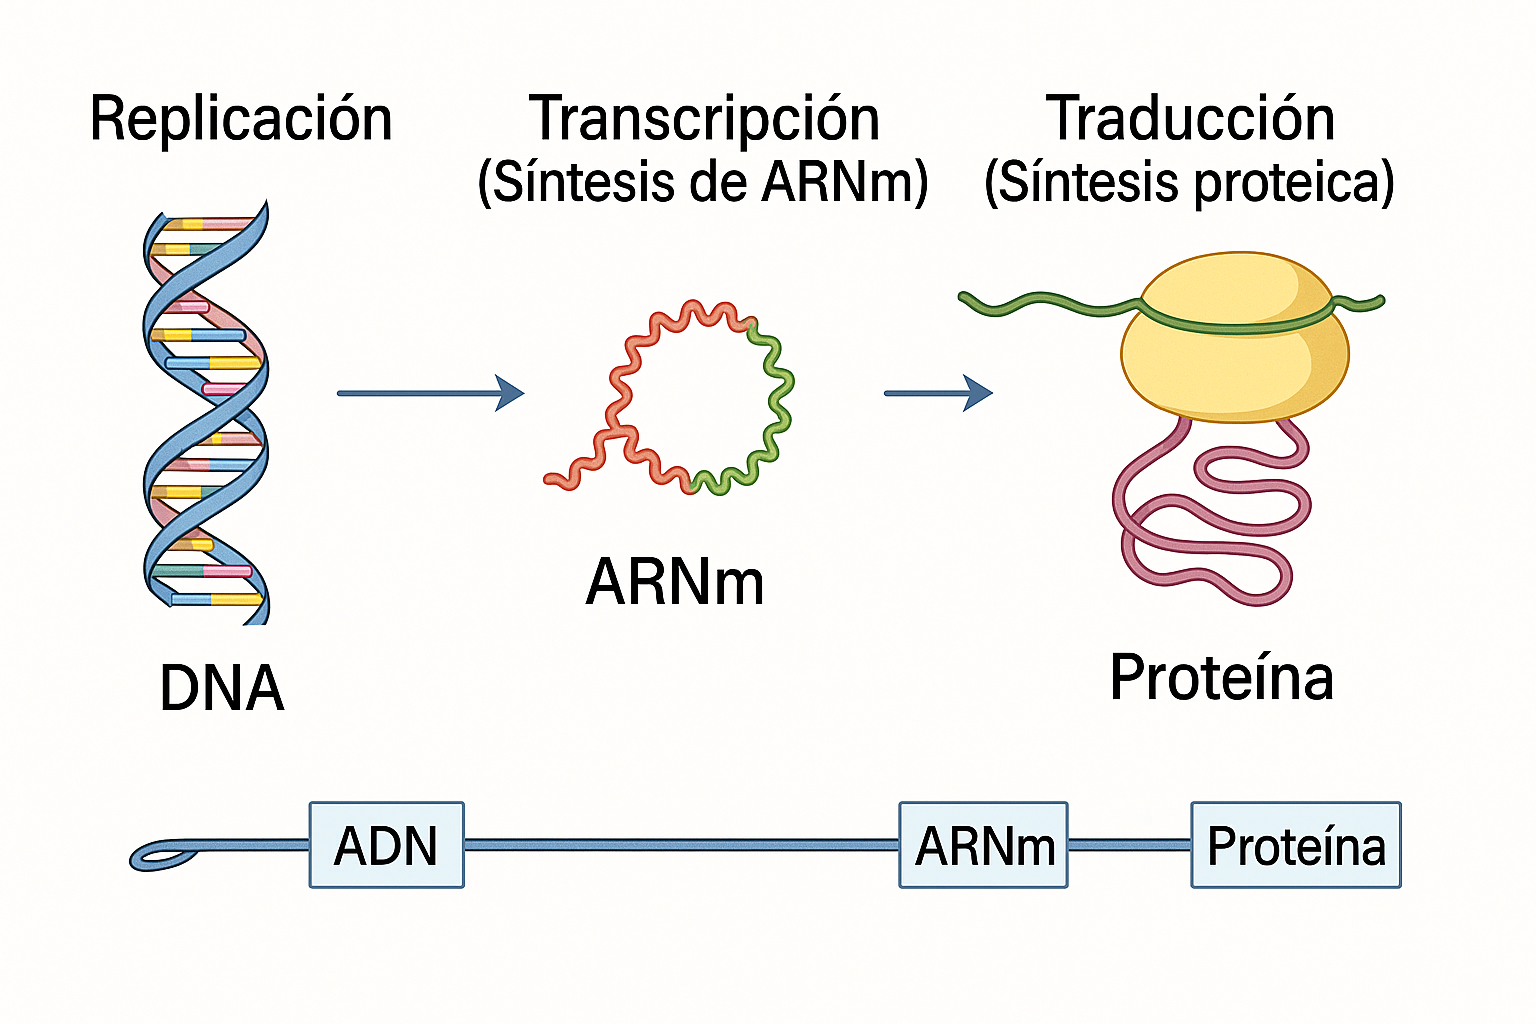
\includegraphics[width=0.9\textwidth]{ADN.png}
   \caption{Procesos genéticos de la síntesis de proteínas.}
   \label{fig:etiqueta_opcional1}
\end{figure}

Sin embargo, el \acs{ADN} no actúa directamente para realizar funciones celulares. En su lugar, esa información debe ser primero transcrita en moléculas de \acs{ARN} (en este la timina se sustituye por uracilo, otra pirimidina), las cuales desempeñan roles clave en la expresión génica. Este proceso, conocido como transcripción, da lugar a diferentes tipos de \acs{ARN}, que luego participan en distintos mecanismos celulares.

Existen dos tipos principales de transcritos que resultan de este proceso: el \acs{ARN} mensajero (\acs{ARN}m), que lleva la información del \acs{ADN} a los ribosomas para la síntesis de proteínas, y el \acs{ARN} no codificante (ARNnc), que, aunque no se traduce en proteínas, cumple funciones esenciales como la regulación génica, la modificación del \acs{ARN}, la estructura de los ribosomas y otras tareas fundamentales para el control celular\cite[p.~254-300]{WAT}. 

El ARN mensajero (ARNm) actúa como intermediario entre el \acs{ADN} y las proteínas de la siguiente manera: mediante el proceso de traducción, los ribosomas convierten cada molécula de \acs{ARN}m en una proteína, es decir, en una secuencia de aminoácidos. Cada proteína adopta una estructura tridimensional compleja y funciones específicas. Gracias a la interacción entre el ADN, \acs{ARN} y proteínas, el genoma es capaz de regular qué células deben crecer, morir y cómo se estructuran, entre otras funciones\cite{RIN}. 


Por esta razón, cada individuo presenta un genoma ligeramente distinto al resto. Estas diferencias son conocidas como variaciones o mutaciones genómicas, y pueden suponer variaciones de un único nucleótido o múltiples nucleótidos. Estos cambios influyen en el fenotipo del individuo y también pueden ser responsables de ciertas enfermedades. 

Se procede a citar los distintos tipos de mutaciones:

\begin{itemize}
   \item SNV: sustitución de una sola base del \acs{ADN} por otra. Es el tipo más común de variación genética en el genoma humano. 
   \begin{itemize}
      \item Sinónima: La sustitución no cambia el aminoácido codificado por el codón, debido a la degeneración del código genético. No suele tener efecto funcional, aunque puede afectar la eficiencia de traducción o el splicing. 
      \item No sinónima: Cambia el aminoácido codificado. Esta a su vez se subdivide en Missense (se sustituye un aminoácido por otro, por lo que puede alterar la función o estructura de la proteína) y Nonsense (introduce un codón de parada prematuro, truncando la proteína, y esta normalmente acaba inactiva o no funcional). 
   \end{itemize}
   
   \item  \acs{INDEL}s (Inserciones y deleciones): Variaciones que implican la inserción o eliminación de un pequeño número de nucleótidos. Son el segundo tipo más común de variación.
   \begin{itemize}
      \item In-frame \acs{INDEL}: El número de nucleótidos es múltiplo de 3. Esto afecta uno o más codones completos, pero no altera el marco de lectura. Puede tener o no efecto funcional. 
      \item Frameshift \acs{INDEL}: El número de nucleótidos no es múltiplo de 3, por lo que altera el marco de lectura de todo el gen a partir del punto del \acs{INDEL}, generando proteínas aberrantes y normalmente no funcionales. 
   \end{itemize}
   \item Copy Number Variation (\acs{CNV}): Amplificaciones o deleciones de segmentos largos del \acs{ADN}. Pueden incluir genes completos o regiones reguladoras. Pueden estar relacionadas con la variabilidad fenotípica, trastornos del desarrollo y enfermedades neuropsiquiátricas\cite{ZHA}.
   \item Structural Variation (\acs{SV}): Alteraciones grandes en la estructura del genoma que incluyen inversiones, translocaciones, inserciones o deleciones mayores.
   \begin{itemize}
      \item Inversiones: Un segmento se invierte dentro del mismo cromosoma. 
      \item Translocaciones: Fragmentos de \acs{ADN} se trasladan a otras posiciones o cromosomas.
      \item Grandes deleciones/duplicaciones: afectan múltiples genes/regiones. 
   \end{itemize}
\end{itemize}


\section{Conceptos básicos de ficheros genéticos}

Las tecnologías de secuenciación de nueva generación (\acs{NGS}) son muy utilizadas hoy en día en investigación genómica y biomédica. Para facilitar el análisis y transferencia de datos, se han definido diferentes formatos de archivos estándar. 

Cuando se secuencia una muestra biológica mediante un sistema de \acs{NGS}, se generan pequeños fragmentos de \acs{ADN} o \acs{ARN} que representan secuencias del genoma, conocidos como lecturas. Estas lecturas se almacenan en archivos de lectura cruda (raw read files). Los formatos más comunes son: \acs{FASTA}, fastq y fasta.gz. 

Después, esas lecturas deben ser alineadas con el genoma de referencia (como el genoma humano), y el resultado de este alineamiento se guarda en archivos SAM (Sequence Alignment Map) o BAM (Binary Alignment Map). 

Por último, a partir de los archivos de alineamiento anteriores, se pueden realizar análisis posteriores para entender la muestra:  

\begin{itemize}
   \item Si el objetivo es identificar mutaciones (como los SNV), esta información se guarda en un archivo con formato \acs{VCF} (Variant Call Format) o BCF (Binary Call Format). 
   \item Si se desea medir la densidad de lecturas en diferentes zonas del genoma, se obtienen archivos con formato Wiggle, BedGraph, BigWig o cWig.
   \item Si se busca definir regiones que estén cubiertas por lecturas (por ejemplo, para identificar exones), los resultados se almacenan en formato bed o bigBed.
\end{itemize}

En este proyecto, nos enfocaremos principalmente en dos de estos formatos: 

\subsection{FASTA}

El formato \acs{FASTA} es un formato de texto estándar para representar secuencias biológicas como \acs{ADN}, \acs{ARN} y proteínas mediante letras. Permite incluir nombres y comentarios de las secuencias. Es simple y permite la manipulación de secuencias usando herramientas de procesamiento de texto\cite{JAV}. Un archivo \acs{FASTA} consta de una o varias secuencias estructuradas de la siguiente manera: una línea de encabezado que debe comenzar con el carácter ‘>’ seguido de un identificador único de secuencia (SeqID), y la secuencia de nucleótidos que puede estar compuesta por una o varias líneas \cite{FAS}.

\begin{table}[H]
   \centering
   \caption{Ejemplo de archivo en formato \acs{FASTA}}
   \begin{tabular}{|l|}
   \hline
   \texttt{>chr1\_example\_sequence} \\ \hline
   \texttt{AGCTGATCGATCGATCGTACGTAGCTAGCTGACT} \\
   \texttt{GCTAGCTAGCATCGATCGTAGCTAGCTAGCTGAC} \\
   \texttt{TAGCTAGCTAGCATCGATCGATCGATCGATCGTA} \\
   \hline
   \end{tabular}
   \label{tabla:FASTA}
   \end{table}
   

Gracias a su estructura sencilla y la compatibilidad con la mayoría de las herramientas bioinformáticas, se ha convertido en un formato estándar por su eficiencia para manipular secuencias biológicas\cite{GEN}

\subsection{VCF}

\acs{VCF} es un formato de archivo de texto utilizado en bioinformática específicamente diseñado para almacenar información sobre variantes genómicas, detectadas mediante procesos de secuenciación del \acs{ADN}. Se trata de un estándar utilizado en múltiples proyectos genómicos a gran escala, como es el 1000 Genome Project\cite{AUT}. Esto es debido a que se trata de un archivo muy estructurado y con capacidad de representar de manera clara y eficaz las variaciones observadas en una o varias muestras, y su facil escalabilidad\cite{EMB}.

Dado que los archivos \acs{VCF} estan diseñados para albergar una gran cantidad de información, existe un formato binario alternativo llamado BCF (Binary Call Format) para facilitar su almacenamiento, transferencia y análisis computacional, ya que es una versión comprimida del anterior. 

Un archivo \acs{VCF} consta de una cabecera y una sección de datos: 

\begin{itemize}
   \item La cabecera incluye un número arbitrario de líneas de metainformación, las cuales van precedidas de \texttt{\#\#}. Estas definen el contenido, las convenciones utilizadas, los tipos de anotaciones y los nombres de las columnas de la sección de datos\cite{DAN}.
      \begin{table}[H]
         \centering
         \caption{Ejemplo de cabecera de un archivo \acs{VCF}}
         \begin{tabular}{|l|}
         \hline
         \texttt{\#\#fileformat=\acs{VCF}v4.2} \\
         \texttt{\#\#FILTER=<ID=PASS,Description="All filters passed">} \\
         \texttt{\#\#INFO=<ID=AF,Number=A,Type=Float,Description="Allele Frequency">} \\
         \texttt{\#\#FORMAT=<ID=GT,Number=1,Type=String,Description="Genotype">} \\
         \texttt{\#CHROM POS ID REF ALT QUAL FILTER INFO FORMAT SAMPLE1 SAMPLE2} \\
         \hline
         \end{tabular}
         \label{tabla:cabeceraVCF}
      \end{table}
      
   \item En la sección de datos, cada fila corresponde a una variante identificada, de la cual se incluye la siguiente información estructurada en diferentes columnas: CHROM y POS describen el cromosoma y la posición de inicio en el genoma donde se encuentra la variante; ID es el identificador único de la variante; REF contiene la base o secuencia de referencia, es decir, el alelo de referencia, que representa la forma más común del fragmento de ADN en esa posición del genoma; ALT recoge una lista de alelos alternativos observados (es decir, otras posibles bases nitrogenadas distintas a la esperada en esa posición), separados por punto y coma si hubiera más de uno; QUAL es la puntuación de calidad de la variante (la confianza en esta); FILTER define el resultado del proceso de filtrado (si la variante pasa los controles de calidad); y por último INFO contiene anotaciones adicionales sobre la variante\cite{EMB}. Además, cuando el archivo \acs{VCF} incluye información de varias muestras, se agregan diferentes campos entre los que destaca FORMAT, lista para definir qué tipo de información se añade para cada muestra. 
      \begin{table}[H]
         \centering
         \caption{Ejemplo de la sección de datos en un archivo VCF}
         \begin{adjustbox}{width=\textwidth}
         \begin{tabular}{|l|r|l|l|l|r|l|l|l|l|l|}
         \hline
         \textbf{CHROM} & \textbf{POS} & \textbf{ID} & \textbf{REF} & \textbf{ALT} & \textbf{QUAL} & \textbf{FILTER} & \textbf{INFO} & \textbf{FORMAT} & \textbf{SAMPLE1} & \textbf{SAMPLE2} \\
         \hline
         3 & 879317 & rs112 & G & A & 99.0 & PASS & AF=0.5;DP=100 & GT:DP & 0/1:48 & 1/1:52 \\
         3 & 879445 & . & T & CTT & 72.5 & PASS & AF=0.25;DP=80 & GT:DP & 0/0:42 & 0/1:38 \\
         3 & 879587 & rs119 & C & T & 85.2 & PASS & AF=0.33;DP=90 & GT:DP & 1/1:45 & 0/1:45 \\
         \hline
         \end{tabular}
         \end{adjustbox}
         \label{tabla:ejemploVCF}
      \end{table}
      
      
      
\end{itemize}



\section{Teoría de la Información}

La Teoría de la Información es una disciplina que estudia la cuantificación, almacenamiento y comunicación de datos, especialmente enfocada en la transmisión de información a través de canales. Fue desarrollada por Claude Shannon y Warren Weaver en los años 40. Sin embargo, su aplicación se ha extendido a otros campos como la informática, la lingüística, o la biología\cite{COV}.

“Una fuente de información se define como un par (S, P) donde S es un alfabeto predefinido y P es una distribución de probabilidad sobre S. Dado que la fuente de información introduce una incertidumbre en la variable aleatoria definida por el alfabeto predefinido, la entropía mide el grado de incertidumbre de dicha variable. También el grado de aleatoriedad en la fuente de información y, en consecuencia, permite estimar las unidades de información necesarias en promedio para codificar todos los valores posibles que puedan darse en la fuente de información.”\cite[p.~3]{ROB}

Para entender mejor esta idea, definiremos unos conceptos clave:  

\subsection{Canal de comunicación }

Un canal de comunicación es el medio físico o digital a través del cual se transmite la información.  

\subsection{Compresión de datos}

La compresión hace referencia a la reducción del tamaño de los datos sin perder información.  

\subsection{Código}

El código es el sistema de símbolos o señales utilizado para representar la información. 

\subsection{Entropía} 

El concepto de entropía se introdujo en el siglo XIX en la termodinámica como una magnitud física que media el grado de desorden en un sistema. En la etapa de 1940, Shanon trasladó este concepto al ámbito de las comunicaciones, ya que definió la entropía como una medida de incertidumbre o sorpresa asociada a un conjunto de mensajes\cite[p.~4]{ROB}. Esta idea fundó lo que se conoce hoy en día como Teoría de la Información. Dada una variable aleatoria X con distribución de probabilidad P, la entropía se define como: 

\[
H(X) = - \sum_{i=1}^{n} p(x_i) \log_2 p(x_i)
\]

La entropía se interpreta como el número promedio de bits necesarios para codificar los resultados de una variable aleatoria. 

\begin{itemize}
   \item Entropía máxima: si una variable aleatoria tiene n resultados igualmente probables, es decir, todos tienen la misma probabilidad de ocurrencia, su entropía vale \( \log_2 n \). 
   \item Entropía mínima: si hay certeza de ocurrencia de un evento, es decir, tiene probabilidad 1 y por lo tanto el resto 0, la entropía vale 0.
\end{itemize}
 
En el contexto de este Trabajo de Fin de Grado, esta idea se aplica a secuencias de \acs{ADN}, donde cada símbolo representa una base nitrogenada (Adenina, Citosina, Timina y Guanina) y la probabilidad de ocurrencia de cada una se mide mediante la frecuencia relativa en una región determinada del genoma. Por ejemplo, calcular la entropía de un conjunto de k-mers en una secuencia de \acs{ADN} podría ayudar a identificar regiones altamente conservadas o variables. Un k-mer es un fragmento de longitud fija k dentro de una secuencia de ADN; es decir, una subsecuencia contigua de k nucleótidos. Analizar la frecuencia de aparición de estos k-mers permite capturar patrones repetitivos o inusuales en el genoma, lo que puede ser especialmente útil para detectar regiones funcionales o alteradas. Estas regiones pueden correlacionarse con funciones biológicas importantes, como promotores, regiones reguladoras, o sitios de mutación frecuentes. 

\subsection{Información}

Los conceptos de entropía e información están relacionados, pero es importante saber distinguirlos. La información es la diferencia entre la máxima entropía (por ejemplo, en una situación de incertidumbre total) y la entropía actual (con cierta cantidad de conocimiento). La información por tanto representa la reducción de incertidumbre:

\[
I(X:Y) = H(X) - H(X \mid Y)
\]

Esta relación se conoce como información mutua y cuantifica la cantidad de información que se obtiene de la variable X al conocer la variable Y. Es fundamental en muchos contextos como el análisis de datos o el análisis genómico, ya que ayuda a conocer las correlaciones entre una base y su contexto, o con otras entidades como proteínas, regiones funcionales o mutaciones. 


\subsection{Modelos de fuentes de Markov}

“Una fuente de información con memoria nula se define como un par (S,P) donde la emisión de cada símbolo \( s_i \) sólo depende de su probabilidad \( p(s_i) \). Una fuente de información con memoria (de orden \( m \)) se define como un par (S,P) de forma que la emisión de cada símbolo \( s_i \) depende de los \( m \) símbolos emitidos con anterioridad, con una probabilidad condicional \( p(s_i \mid s_{i1}, s_{i2}, \dots, s_{im}) \).”\cite[p.~19]{ROB}

Las fuentes de información básicas no tienen memoria, es decir, en el cálculo de la probabilidad de una determinada base no se tienen en cuenta las bases anteriores. Sin embargo, en genómica, el \acs{ADN} no es del todo aleatorio, ciertas bases tienden a seguir a otras con mayor probabilidad, lo que sugiere que un modelo de Fuente de Markov puede ser más realista. 


Una Fuente de Markov (o fuente de información con memoria) se define como un sistema donde la probabilidad de que ocurra cada símbolo depende de los símbolos que le preceden. Estas nuevas probabilidades se consiguen gracias a la matriz de probabilidades de transición entre estados (los estados de una fuente de Markov de orden \( m \) serán todas las posibles combinaciones \( n \) de longitud \( m \) símbolos, es decir, \( n^m \)). Además, dada una fuente de Markov de orden \( m \), se puede establecer su diagrama de estados, que muestra los estados y las probabilidades condicionales entre ellos\cite[p.~20]{ROB}.

\begin{itemize}
   \item Una fuente de Markov diremos que es ergódica si todos los estados son alcanzables (observables) desde cualquier estado.
   \item Una fuente de Markov es homogénea si las probabilidades de transición entre estados no cambian a lo largo del tiempo.
   \item Una fuente de Markov está en estado estacionario si la probabilidad de observación de sus estados no cambia a lo largo del tiempo. Las probabilidades se pueden obtener mediante la ecuación $\pi = \pi \times \Pi$, donde $\pi$ es el vector de probabilidad de los estados y $\Pi$ es la matriz de probabilidades condicionales (estocástica).
\end{itemize}

\begin{figure}[H]
   \centering
   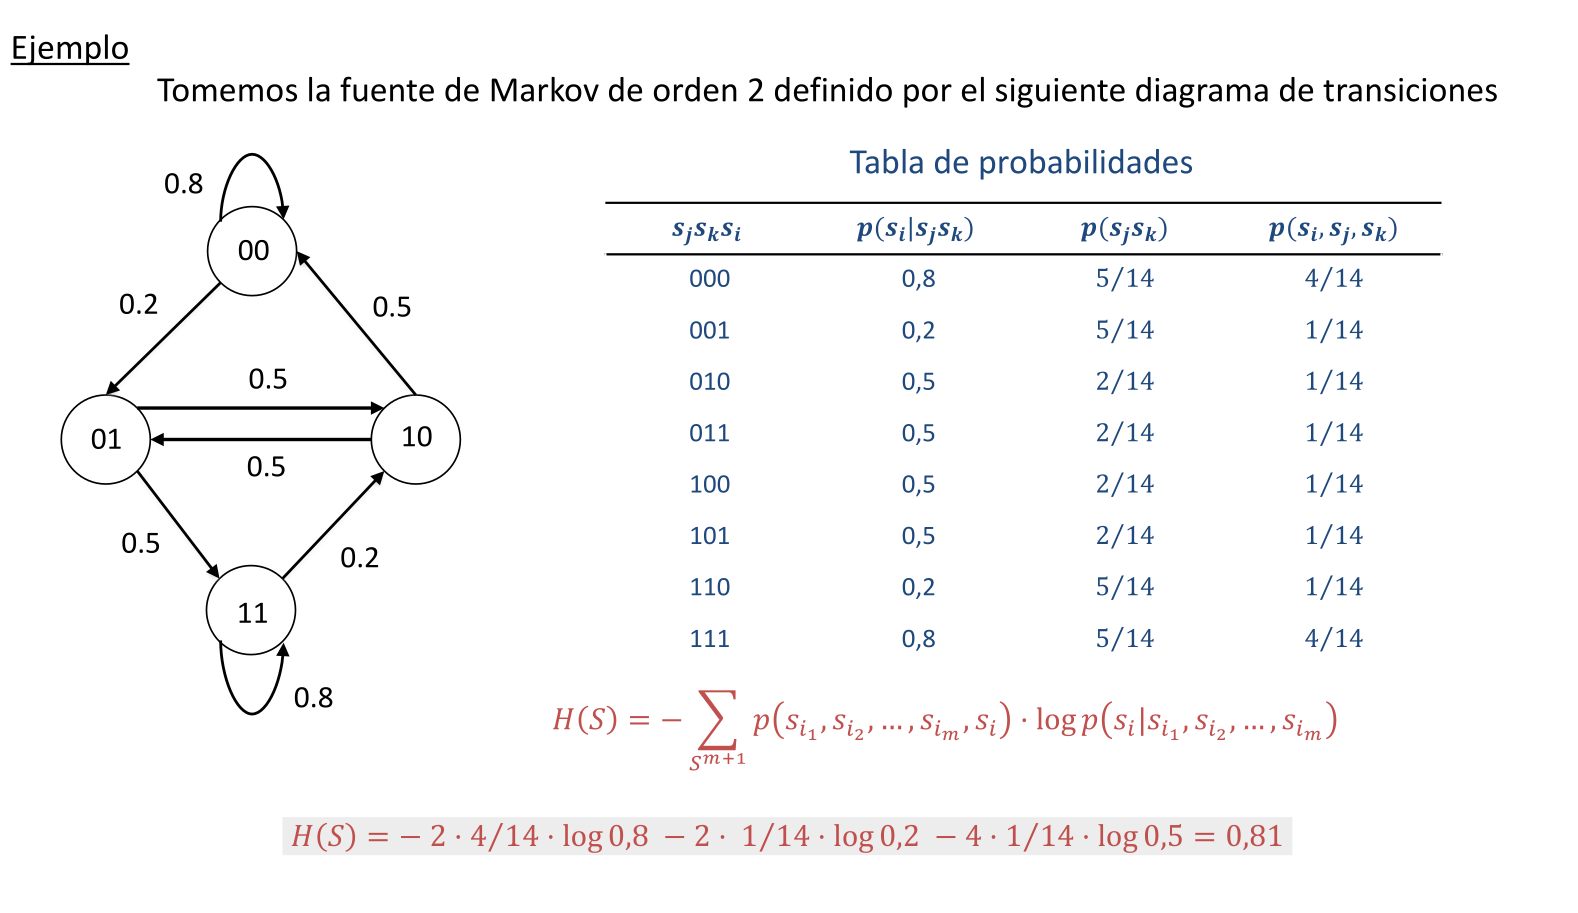
\includegraphics[width=0.9\textwidth]{entropia_markov.png}
   \caption{Ejemplo de cálculo de entropía condicional.}
   \label{fig:etiqueta_opcional}
\end{figure}

Por lo tanto, en una fuente de Markov de orden m, la probabilidad de ocurrencia de un símbolo, depende de los (m-1) símbolos anteriores. Cuanto mayor sea el orden (m), más información del contexto se incluye, y, en consecuencia, menores valores de entropía. Esto significa que modificar los valores de m, puede revelar patrones o regiones funcionales dentro de la secuencia dada. 


\chapter{Análisis del problema}

\section{Análisis del marco legal y ético}

Este Trabajo de Fin de Grado implica el análisis de datos genómicos reales pertenecientes a pacientes con enfermedades raras, concretamente la \acs{RP}, proporcionados por el Grupo de Investigación en Biomedicina Molecular, Celular y Genómica del \acs{IIS} La Fe. Debido a esto, resulta esencial garantizar el cumplimiento con la normativa vigente de protección de datos personales.

El tratamiento de información genética está regulado por el Reglamento General de Protección de Datos (\acs{RGPD}) y la Ley Orgánica 3/2018, de Protección de Datos Personales y garantía de los derechos digitales (\acs{LOPDGDD}). En este sentido, para garantizar el cumplimiento, los datos utilizados en este trabajo han sido previamente anonimizados. Los archivos utilizados en este proyecto no incluyen información identificativa directa de los pacientes, y han sido tratados exclusivamente para fines de investigación y desarrollo académico. Además, todo el análisis se ha llevado a cabo en un entorno local y seguro, sin almacenar ni transmitir datos a ningún tipo de servidor externo.

En cuanto al software desarrollado, tanto la parte de la lógica como la interfaz han sido implementadas desde cero, y se ha tenido especial cuidado en respetar las licencias y derechos de todos los recursos externos utilizados (librerías, datasets, imágenes…), citando las fuentes correctamente cuando ha sido necesario. Los datos de referencia, como los archivos FASTA, han sido obtenidos de bases de datos públicas (\acs{NCBI}), y los archivos \acs{VCF} clínicos han sido facilitados en el marco de una colaboración académica con la Universitat Politècnica de València (\acs{UPV}).

Por último, cabe destacar que la aplicación no accede a internet ni recopila información del usuario más allá de los parámetros que introduce. La ejecución se hace de forma local, lo cual minimiza cualquier riesgo de seguridad o privacidad adicional y facilita que el desarrollo del proyecto se haga de forma responsable tanto desde el punto de vista legal como ético.


\section{Identificación y análisis de soluciones}

La hipótesis de partida se basa en la idea de que la entropía de una secuencia de \acs{ADN} experimenta cambios significativos en las regiones donde puede haber mutaciones patogénicas. Estas regiones de valores anómalos entropía podrían coincidir con las zonas funcionales asociadas a enfermedades raras. 

El análisis se estructura en tres casos de estudio diferentes, cada uno enfocado a detectar patrones distintos en la secuencia:

\subsection{Caso 1: Cálculo de entropía en ventanas deslizantes}

En este primer análisis, se calcula la entropía en ventanas deslizantes de tamaño w a lo largo de la secuencia genómica. Una ventana deslizante es un segmento de longitud fija que se mueve a lo largo de la secuencia permitiendo analizar de manera local diferentes regiones del genoma. El desplazamiento de la ventana (step size) puede ser de un solo nucleótido o ajustarse según lo que se desee en el análisis (en este trabajo se ha utilizado un desplazamiento de 1). Por ejemplo, si se utiliza una ventana de tamaño w = 10 y un desplazamiento de 1, la primera ventana cubrirá las posiciones 1 a 10, la segunda de 2 a 11, la tercera de 3 a 12, y así sucesivamente hasta el final de la secuencia. El objetivo es comparar las variaciones de entropía entre la secuencia de referencia y la secuencia mutada.

La entropía $H$ para cada ventana se calcula como:

\[
H = - \sum p(kmer) \cdot \log_2 p(kmer)
\]

Donde:

\begin{itemize}
   \item $p(kmer)$ es la probabilidad de aparición de un k-mer dentro de la ventana.
   \item La probabilidad se calcula como la fracción de la frecuencia de ese k-mer entre el número de tipos distintos de k-mer en la ventana.
\end{itemize}

Se recorren ambas secuencias (referencia y mutada) y se calcula la entropía de cada ventana. Posteriormente, se representan gráficamente las entropías de ambas secuencias a lo largo de la posición genómica para detectar picos o variaciones significativas.

\subsubsection{Ejemplo}

Se tiene la siguiente secuencia genómica simplificada de ADN: ATGCGATCGAACGT. Se define una ventana deslizante de tamaño $w = 8$ con desplazamiento $1$, lo cual permite obtener las siguientes sub-secuencias (ventanas):

\begin{itemize}
    \item Ventana 1: \texttt{ATGCGATC}
    \item Ventana 2: \texttt{TGCGATCG}
    \item Ventana 3: \texttt{GCGATCGA}
    \item Ventana 4: \texttt{CGATCGAA}
    \item Ventana 5: \texttt{GATCGAAC}
    \item Ventana 6: \texttt{ATCGAACG}
    \item Ventana 7: \texttt{TCGAACGT}
\end{itemize}

Tomamos como ejemplo la primera ventana: ATGCGATC. Dentro de esta ventana se extraen los trigrama (k-mers de tamaño 3), con desplazamiento 1:

\begin{itemize}
    \item ATG
    \item TGC
    \item GCG
    \item CGA
    \item GAT
    \item ATC
\end{itemize}

En este caso, cada trigrama aparece una sola vez en la ventana, por lo que todas las probabilidades son iguales:

\[
p(\text{k-mer}) = \frac{1}{6}
\]

Ahora, se procede a calcular la entropía sustituyendo en la fórmula:

\[
H = - \sum_{i=1}^{n} p(k_i) \cdot \log_2 p(k_i)
\]

\[
H = - 6 \cdot \left( \frac{1}{6} \cdot \log_2 \frac{1}{6} \right) = - \log_2 \frac{1}{6} \approx \log_2 6 \approx 2.585
\]


\subsection{Caso 2: Cálculo de entropía basada en probabilidades condicionales (Modelo de Markov)}

En el segundo análisis, se utiliza un enfoque más avanzado basado en modelos de Markov de orden K para calcular la entropía condicional entre k-mers. Esta K no debe ser confundida con k minúscula, la cual hace referencia al tamaño del k-mer. Para ello, ahora los k-mers forman el conjunto de datos a partir del cual se van a obtener los estados iniciales, finales, transiciones y sus probabilidades. Por esta razón, el orden de la fuente de Markov (K) debe ser siempre menor al tamaño de k-mer (k).
\subsubsection{Creación de la fuente de Markov}

Se construye una fuente de Markov que permite modelar la secuencia como una cadena de estados, donde:

\begin{itemize}
   \item El alfabeto está formado las diferentes bases nitrogenadas {A, C, G, T}.
   \item Los estados iniciales se corresponden con los primeros caracteres de los k-mers.
   \item Los estados finales corresponden a los últimos caracteres de cada k-mer.
   \item Las transiciones representan la concatenación de bases adyacentes.
\end{itemize}


Por ejemplo, dado un conjunto de k-mers S = ACGT, ACCG, se define el siguiente modelo de segundo orden:

\begin{itemize}
   \item Alfabeto: {A, C, G, T}.
   \item Estados iniciales: {A}.
   \item Estados finales: {T, G}.
   \item Transiciones: {AC, CG, GT, CC}.
\end{itemize}


\subsubsection{Cálculo de Probabilidades de Transición}
Una vez definidos los elementos de la fuente de Markov, se recorren las secuencias y se cuentan las ocurrencias de cada transición. Con esta información, se calcula la probabilidad de transición desde un estado s a otro estado t como:

\[
p(s \to t) = \frac{\text{Número de transiciones de } s \to t}{\text{Total de transiciones desde } s}
\]

Si una transición no existe, se le asigna una probabilidad muy baja para evitar problemas en el cálculo del logaritmo.

\subsubsection{Cálculo de Entropía Condicional}

Se desliza una ventana de tamaño w sobre la secuencia y, dentro de esta ventana, se analizan las transiciones de tamaño k para calcular la contribución a la entropía condicional de cada transición.

La entropía total de la ventana se calcula restando las contribuciones de todas las transiciones observadas.

\subsubsection{Ejemplo}

A modo de ejemplo, se tiene una secuencia genómica correspondiente a una ventana de tamaño 10: ATGCACGCAG, el tamaño de kmer es 4, y la orden de la fuente de Markov (k) es 3. A partir de esta secuencia se extraen los siguientes k-mers de tamaño 4: 
\[
\{ATGC,\ TGCA,\ GCAC,\ CACG,\ ACGC,\ CGCA,\ GCAG\}.
\]
Por lo tanto, se formalizan estos datos:

\begin{itemize}
   \item Orden de la fuente: k = 3.
   \item Tamaño de k-mer = 4.
   \item Conjunto de datos: S = {ATGC, TGCA, GCAC, CACG, ACGC, CGCA, GCAG}.
   \item Alfabeto: \( \Sigma = \{A, T, G, C\} \).
   \item Estados iniciales: I = {AT, TG, GC, CA, AC, CG}.
   \item Estados finales: F = {GC, CA, AC, CG, AG}.
   \item Transiciones: T = {ATG, TGC, GCA, CAC, ACG, CGC, GCA, CAG}.
\end{itemize}

A partir de estos datos, se obtiene el siguiente diagrama de transiciones:

\begin{figure}[H]
   \centering
   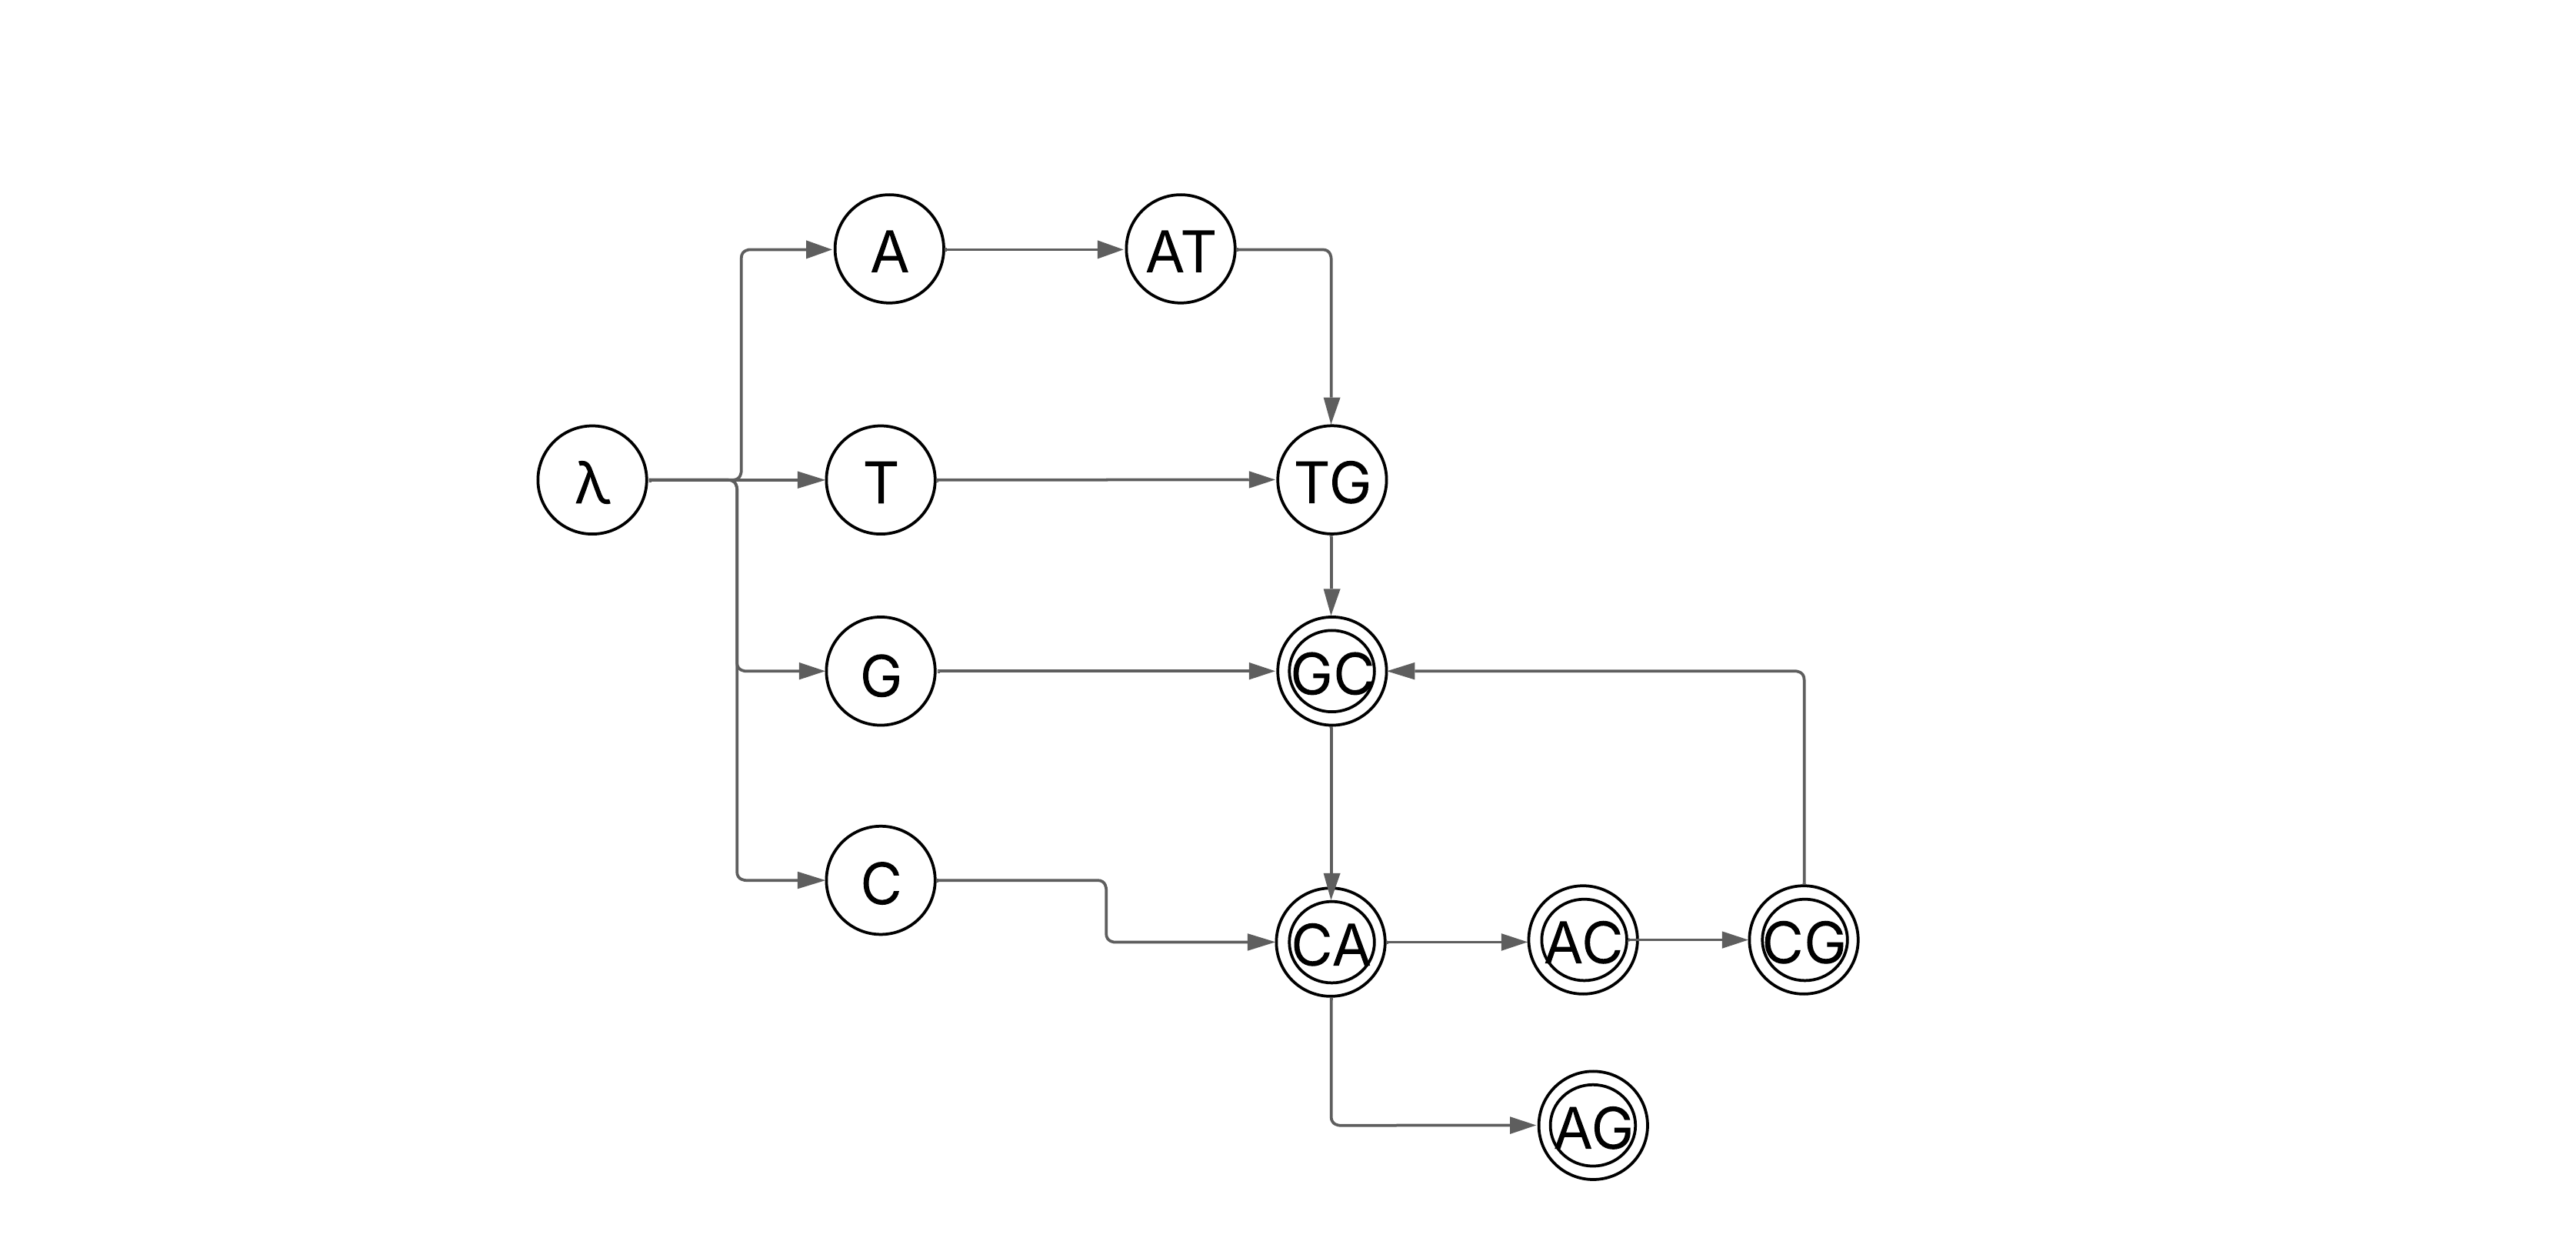
\includegraphics[width=1.1\textwidth]{automataMarkov.png}
   \caption{Diagrama de transiciones a partir de la fuente de Markov.}
   \label{fig:etiqueta_opcional114}
\end{figure}

A continuación, para calcular la tabla de probabilidades, se necesita contar las transiciones salientes por estado (el total de transiciones es 7):

\begin{itemize}
   \item ATG \(\rightarrow\) 1 transición
   \item TGC \(\rightarrow\) 1 transición
   \item GCA \(\rightarrow\) 2 transiciones
   \item CAC \(\rightarrow\) 1 transición
   \item ACG \(\rightarrow\) 1 transición
   \item CGC \(\rightarrow\) 1 transición
\end{itemize}



\begin{table}[H]
\centering
\renewcommand{\arraystretch}{1.5} % Espacio entre filas
\setlength{\tabcolsep}{12pt}      % Espacio entre columnas
\large                             % Tamaño de fuente más grande
\caption{Probabilidades de transición entre estados}
\label{tabla:transiciones}
\begin{tabular}{|c|c|c|c|}
\hline
\textbf{\( s_j s_k s_i \)} & \textbf{\( p(s_i \mid s_j s_k) \)} & \textbf{\( p(s_j s_k) \)} & \textbf{\( p(s_i, s_j, s_k) \)} \\
\hline
ATG & 1.0 & \( \frac{1}{7} \) & \( \frac{1}{7} \) \\
TGC & 1.0 & \( \frac{1}{7} \) & \( \frac{1}{7} \) \\
CAC & 0.5 & \( \frac{2}{7} \) & \( \frac{1}{7} \) \\
CAG & 0.5 & \( \frac{2}{7} \) & \( \frac{1}{7} \) \\
GCA & 1.0 & \( \frac{1}{7} \) & \( \frac{1}{7} \) \\
ACG & 1.0 & \( \frac{1}{7} \) & \( \frac{1}{7} \) \\
CGC & 1.0 & \( \frac{1}{7} \) & \( \frac{1}{7} \) \\
\hline
\end{tabular}
\end{table}


El siguiente paso consiste en calcular la entropía condicional de la ventana sustituyendo los valores en la siguiente fórmula:
\[
H(X \mid Y) = - \sum_{i,j} p(s_i, s_j, s_k) \log_2 p(s_i \mid s_j s_k)
\]

\[
H = - \left(
\frac{1}{7} \log_2 1.0 +
\frac{1}{7} \log_2 1.0 +
\frac{1}{7} \log_2 0.5 +
\frac{1}{7} \log_2 0.5 +
\frac{1}{7} \log_2 1.0 +
\frac{1}{7} \log_2 1.0 +
\frac{1}{7} \log_2 1.0
\right)
\]

\[
H = - \left(
\frac{1}{7} \cdot 0 +
\frac{1}{7} \cdot 0 +
\frac{1}{7} \cdot (-1) +
\frac{1}{7} \cdot (-1) +
\frac{1}{7} \cdot 0 +
\frac{1}{7} \cdot 0 +
\frac{1}{7} \cdot 0
\right)
\]

\[
H = - \left( \frac{-2}{7} \right) = \frac{2}{7} \approx 0.2857 \text{ bits}
\]


\subsection{Caso 3: Cálculo de densidad de mutaciones}

En este tercer análisis, se estudia la densidad de mutaciones presentes en las regiones cercanas a cada variante detectada en el archivo \acs{VCF}.

Para ello, se toma una ventana de tamaño 2L centrada en cada mutación, es decir, se consideran L posiciones antes y L posiciones después de la posición de la mutación. Dentro de esta ventana, se cuenta el número de mutaciones existentes. Este procedimiento se repite para cada mutación presente en el archivo \acs{VCF}.

El resultado se almacena en una lista que posteriormente se utiliza para generar un gráfico de densidad de mutaciones. Este gráfico representa las zonas con mayor concentración de variantes, lo cual podría indicar regiones funcionales afectadas.

\subsubsection{Ejemplo}

Tras procesar un archivo \acs{VCF}, se obtienen las siguientes posiciones de variantes genéticas en una región del genoma:

\[
\{1000,\ 1220,\ 1340,\ 1500,\ 3050,\ 8000\}
\]

Para estudiar la densidad de mutaciones, es necesario definir una ventana simétrica de tamaño $2L$, centrada en cada mutación. En este caso, se toma $L = 200$. De este modo para cada mutación se considera el rango: $[p - 200,\ p + 200]$

donde $p$ es la posición de la mutación.

Por ejemplo, para la mutación en la posición $1500$, se define la ventana $[1300,\ 1700]$. Dentro de esta ventana, se encuentra dentro del rango la mutación en $1340$ y la de $1500$, por lo que la densidad sería $2$. Realizando este procedimiento para todas las posiciones, se obtendría la siguiente lista de densidades:

\[
\{1,\ 3,\ 3,\ 2,\ 1,\ 1\}
\]

donde cada valor indica cuántas mutaciones se encuentran en la vecindad de cada variante.



\chapter{Diseño de la solución }


\section{Tecnologías utilizadas}

\subsection{Entorno de Trabajo}

El entorno de desarrollo se basa en el sistema operativo Linux, ya que muchas de las bibliotecas necesarias para el análisis de archivos \acs{VCF}, como vcfpy, no tienen soporte en Windows. Para ello, se utiliza:
\begin{itemize}
   \item WSL (Windows Subsystem for Linux) en máquinas con sistema Windows.
   \item Ubuntu directamente instalado en el equipo de trabajo de la oficina.
\end{itemize}

Como gestor de entornos y dependencias se emplea Anaconda, una distribución de Python orientada a ciencia de datos, bioinformática y aprendizaje automático. Anaconda incluye numerosas librerías útiles como numpy, pandas, matplotlib, scikit-learn, entre otras, y permite la creación de entornos virtuales aislados.

\subsection{Archivos necesarios}

\subsubsection{Archivos FASTA}

El archivo \acs{FASTA} es un formato estándar utilizado para almacenar secuencias de \acs{ADN}, \acs{ARN} o proteínas. Este formato de texto simple presenta las secuencias de interés precedidas por una línea de cabecera que comienza con el carácter > seguido de un identificador o descripción de la secuencia. 

En el presente trabajo, los archivos \acs{FASTA} utilizados deben corresponder al ensamblaje genómico GRCh37.p13, disponible en la base de datos \acs{NCBI} (National Center for Biotechnology Information). Cada archivo \acs{FASTA} corresponde a un cromosoma específico de los 46 cromosomas principales del genoma humano. 

Se ha realizado mediante descarga local de estos archivos, ya que el acceso directo a las secuencias mediante peticiones a \acs{NCBI} puede generar errores por limitaciones de memoria RAM en la ejecución del programa. 

\subsubsection{Archivos VCF}

El formato \acs{VCF} (Variant Call Format) es un tipo de archivo utilizado para almacenar variantes genómicas identificadas. De aquí nos interesan especialmente: 

\begin{itemize}
   \item Líneas de metainformación. 
   \item Una línea de encabezado.
   \item Líneas de datos, donde cada línea describe una variante concreta. 
\end{itemize}

Cada variante contiene información sobre la posición en el genoma, el cromosoma, la base de referencia, la base alternativa, así como otros datos asociados a la calidad y características de la variante. De los tipos de variantes estudiados en la sección de fundamentos, los presentes en el archivo \acs{VCF} con el que trabajamos son los siguientes: 

\begin{itemize}
   \item \acs{SNP}s. 
   \item Inserciones. 
   \item Deleciones.
\end{itemize}

Por último, de los archivos \acs{VCF} extraeremos la siguiente información esencial: 

\begin{itemize}
   \item Cromosoma en el que se encuentra la variante.
   \item Posición de la variante dentro del cromosoma.  
   \item Base de la secuencia de referencia (alelo de referencia).
   \item Base correspondiente a la secuencia mutada (alelo alternativo).
\end{itemize}
 

\subsection{Librerías utilizadas}

Durante el desarrollo de este \acs{TFG}, ha sido necesario apoyarse en algunas herramientas que requerían la instalación de ciertas librerías presentes para Python, tanto para el procesamiento y análisis del genoma como para la visualización de los distintos gráficos y el desarrollo de la interfaz de usuario. A continuación, se describen las principales librerías utilizadas y su aportación al proyecto:

\begin{itemize}
   \item Bio (biopython) es la librería por excelencia para la bioinformática, utilizada para acceder a las bases de datos del \acs{NCBI} (mediante BIO.Entrez), y para la lectura y análisis de los archivos que contienen las secuencias genómicas en formato \acs{FASTA} (mediante Bio.SeqIO).
   \item Vcfpy es una librería creada para Python 3, y especializada en el manejo de archivos \acs{VCF}. Esta permite leer, analizar y escribir los archivos con mutaciones de manera estructurada y computacionalmente eficiente, y extraer de manera sencilla e intuitiva la información que se requiere.
   \item Matplotlib es una de las librerías más utilizadas de Python, y se encarga de la generación de gráficos. En este caso se emplea para visualizar de manera clara tres listas: la entropía simple, la entropía generada a partir de fuentes de Markov, y la densidad de mutaciones en la secuencia genómica. Además, se ha configurado un backend (TkAgg) para poder trabajar sin interfaz gráfica, de manera que genera imágenes exportables (en formato png). Por último, se hace uso de matplotlib.ticker, que es un módulo auxiliar que permite personalizar los ejes y formatos numéricos en los gráficos generados.
   \item Pandas es una librería para el análisis y manipulación de datos en forma de tablas, que se utiliza para gestionar y mostrar la información extraída de los archivos \acs{VCF} y almacenar resultados intermedios, como mutaciones no aplicadas.
   \item Numpy es la biblioteca utilizada para lograr la optimización en los cálculos numéricos. En este contexto se usa para operaciones como el cálculo de la entropía simple y la entropía basada en modelos de Markov, ya que permite manejar grandes volúmenes de datos genómicos de forma eficiente.
   \item Streamlit es una librería de Python de código abierto que facilita la creación y el intercambio de aplicaciones web para la ciencia de datos y el Machine Learning. Es una forma rápida y sencilla de convertir código Python en una aplicación web interactiva, sin necesidad de conocimientos previos de desarrollo web . En este proyecto, Streamlit facilita al usuario la carga de archivos \acs{VCF}, la selección del cromosoma de estudio y la visualización de resultados gráficos y tabulares, sin necesidad de conocimientos técnicos avanzados.
\end{itemize}

\begin{figure}[H]
      \centering
      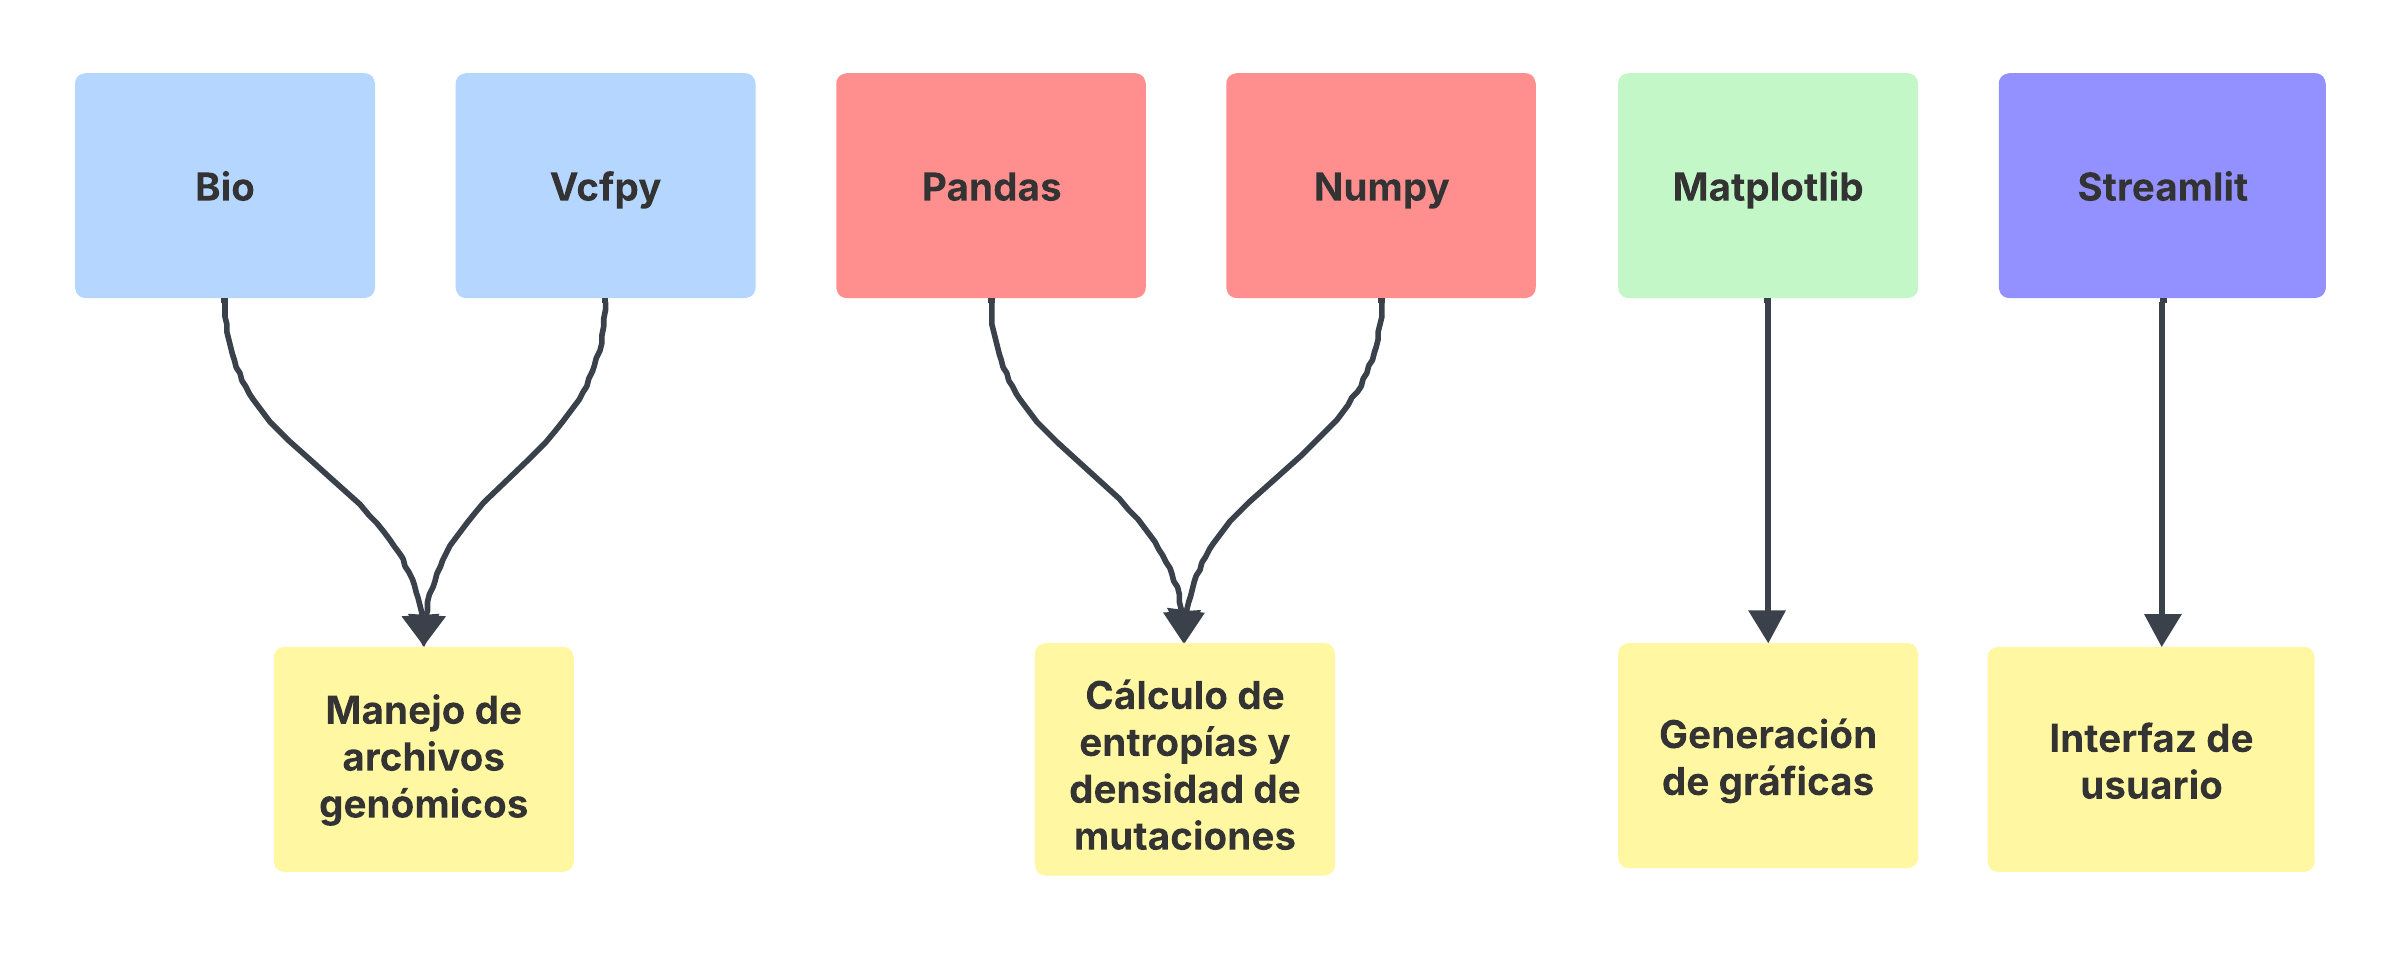
\includegraphics[width=0.9\textwidth]{librerias.png}
      \caption{Diagrama de las librerías utilizadas y su relacion con los diferentes módulos.}
      \label{fig:etiqueta_opcional200}
   \end{figure}


\section{Arquitectura del sistema}

La arquitectura del sistema desarrollado en este Trabajo de Fin de Grado se estructura en base a una interfaz que se comunica con la parte lógica de análisis bioinformático. El diseño modular en diferentes archivos permite abstraer al usuario de los procesos complejos como la aplicación de variantes genéticas, el cálculo de entropía y el análisis de patrones, además de mantener un código organizado, reutilizable y más fácil de mantener o ampliar. 

 

Por lo tanto, la aplicación está dividida en dos componentes principales: 

\begin{itemize}
   \item Una interfaz de usuario (archivo interfaz.py): Desarrollada con la biblioteca Streamlit, permite al usuario interactuar con el sistema mediante menús desplegables, campos de entrada y botones. Desde aquí se cargan los datos, se configuran los parámetros de análisis y se visualizan o descargan los resultados. 
   \item La lógica de aplicación (archivo back.py): Contiene las funciones que procesan los datos genómicos, aplican las mutaciones, calculan entropía (simple y condicional), construyen fuentes de Markov y generan los gráficos. 
\end{itemize}

El flujo general está diseñado para permitir la carga eficiente de los datos genómicos y mutaciones, su procesamiento y la visualización de resultados. 

\subsection{Carga de Datos}

El sistema comienza con la selección de un número de cromosoma por parte del usuario. A partir de este número, la aplicación busca automáticamente el archivo de referencia correspondiente en formato \acs{FASTA}, lo cual simplifica el uso del sistema y reduce errores. Del mismo modo, el usuario debe subir un archivo \acs{VCF} con las variantes genéticas de la muestra que desee. Además, se da la opción de modificar los principales parámetros para el análisis. 

Si no se encuentra el archivo \acs{FASTA} correspondiente, o el archivo con las mutaciones no tiene extensión .vcf, se informa al usuario y se detiene el proceso. Esto garantiza que el sistema solo se ejecuta cuando todos los elementos necesarios están presentes. 

\subsection{Análisis de Secuencia Genómica}

A continuación, se lleva a cabo el núcleo del análisis, dividido en tres módulos: 


\begin{itemize}
   \item Cálculo de entropía en ventanas deslizantes: Se desliza una ventana de tamaño w a lo largo de la secuencia genómica (tanto de referencia como mutada) y se calcula la entropía en cada segmento usando la fórmula de Shannon. 
   \item Densidad de mutaciones: Se analiza la distribución de mutaciones en la secuencia mediante una ventana de tamaño 2L centrada en cada variante detectada y se contabiliza el número de mutaciones en dicho intervalo. 
   \item Entropía basada en modelos de Markov: Se construye un modelo de Fuente de Markov de orden k para representar la secuencia como una cadena de estados. A partir de las transiciones, se calculan probabilidades condicionales y, con ellas, se evalúa la entropía condicional. 
\end{itemize}

\subsection{Visualización y Exportación de Resultados }

Tras finalizar el análisis, el sistema genera varios gráficos: 

\begin{itemize}
   \item Entropía simple de la secuencia de referencia y mutada. 
   \item Entropía condicional o de Markov de la secuencia de referencia y mutada. 
   \item Densidad de mutaciones en la secuencia. 
\end{itemize}

Además, se exportan los siguientes archivos para descarga: 
   \begin{itemize}
   \item Fuente de Markov de la secuencia original y de la secuencia mutada. 
   \item Archivo \acs{VCF} con las mutaciones que no se han podido aplicar. 
   \item Archivo comprimido .zip con todos los resultados. 
\end{itemize}

\begin{figure}[H]
      \centering
      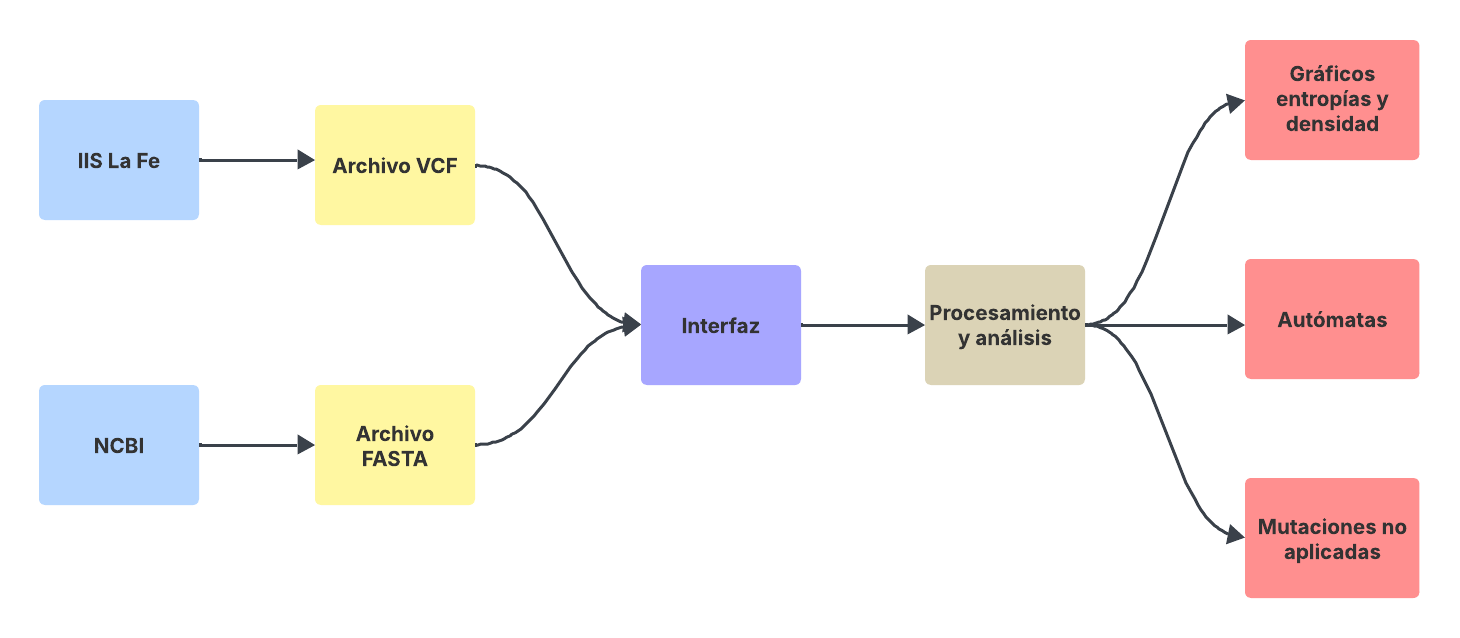
\includegraphics[width=0.9\textwidth]{Diagramas de flujo.png}
      \caption{Diagrama de flujo del sistema.}
      \label{fig:etiqueta_opcional5}
   \end{figure}



\chapter{Desarrollo}

\section{Importación de librerías y configuración inicial }

En primer lugar, se realizan importaciones de librerías necesarias para ejecutar distintas funciones en el análisis genómico y se realiza una configuración inicial del servidor de Streamlit. 

En back.py, el archivo que contiene la lógica de la aplicación, se hace uso de diversas bibliotecas necesarias para recuperar secuencias genómicas, analizarlas, generar gráficos, y trabajar con datos genómicos en diversos formatos. Se usan módulos estándar como math y time, y otros especializados como matplotlib para generar gráficos (aunque configurado para un backend sin interfaz gráfica con TkAgg), pandas y numpy para análisis de datos, y Bio de Biopython para acceder a bases de datos biológicas del \acs{NCBI}. También se importa vcfpy para manejar archivos \acs{VCF} (usados en genómica para representar variantes), y requests para hacer solicitudes HTTP. 

\begin{figure}[H]
      \centering
      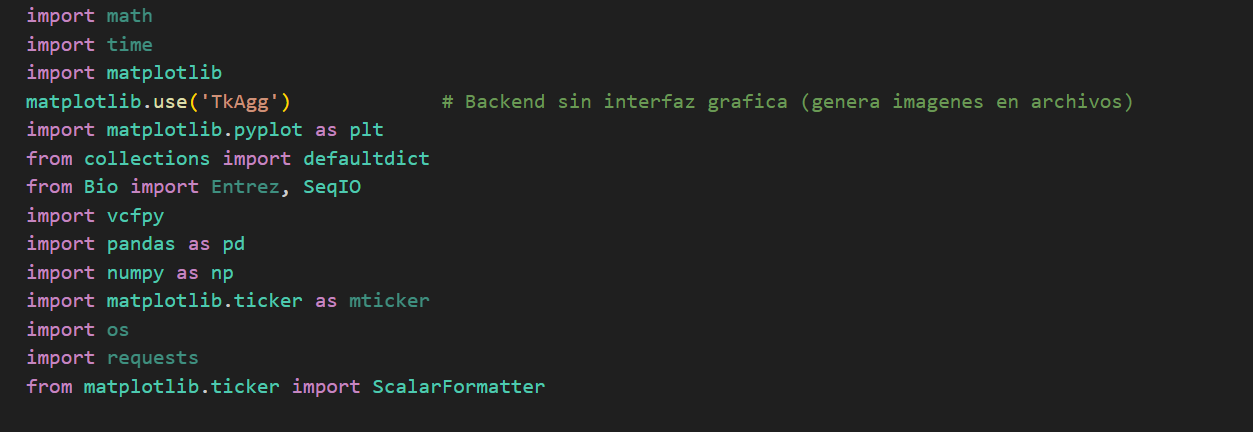
\includegraphics[width=0.9\textwidth]{Capturaback.PNG}
      \caption{Fragmento de código de importación de librerías en back.py}
      \label{fig:etiqueta_opcional125}
   \end{figure}

En interfaz.py, se importan los módulos necesarios para construir la interfaz web con Streamlit, la herramienta de Python para crear aplicaciones interactivas. Se importa st de streamlit para generar la UI, AnalizadorGenomico desde el archivo back.py (que contiene la lógica), y bibliotecas estándar como pandas para manejo de datos, os para operaciones del sistema de archivos, y zipfile para comprimir archivos.  

\begin{figure}[H]
      \centering
      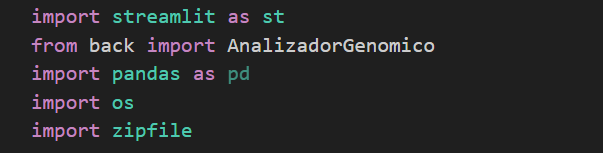
\includegraphics[width=0.7\textwidth]{Capturainterfaz.PNG}
      \caption{Fragmento de código de importación de librerías en interfaz.py}
      \label{fig:etiqueta_opcional126}
   \end{figure}

Adicionalmente, se ha añadido el archivo config.toml en la carpeta streamlit, estableciendo el parámetro maxUploadSize = 1000 dentro de la sección [server]. Esto significa que se ha aumentado el límite máximo de tamaño de archivo que el usuario puede subir a la aplicación a 1 GB, lo cual es necesario para poder trabajar con archivos genómicos grandes como las secuencias genómicas o los \acs{VCF}s. 


\section{Lectura de las mutaciones presentes en el archivo \acs{VCF}}

En segundo lugar, se realiza la lectura del archivo \acs{VCF} correspondiente a los pacientes que presentan una determinada enfermedad rara (en este caso retinosis pigmentaria). 

Para ello, se utiliza una librería específica de Python (vcfpy), que permite extraer de manera estructurada los datos contenidos en el archivo. El programa recorre cada línea del \acs{VCF} (ignorando las líneas de encabezado) y obtiene los datos fundamentales de cada mutación. Sin embargo, no necesitamos obtener los detalles de todas las mutaciones, por lo que se realiza un filtrado para obtener solo las mutaciones que se encuentren en el cromosoma especificado por el usuario. 


\section{Almacenamiento de las mutaciones en una estructura de datos adecuada}

Una vez extraídas las mutaciones del archivo \acs{VCF}, se almacenan en un diccionario de Python (ya que permite un acceso rápido y una organización estructurada y eficiente), de tal manera que cada mutación queda registrada mediante los siguientes campos: 

\begin{itemize}
   \item Cromosoma en el que se encuentra la variante.
   \item Posición exacta dentro del cromosoma.
   \item Base de la secuencia de referencia.
   \item Base correspondiente a la secuencia mutada.
\end{itemize}

\section{Extracción de la secuencia de referencia del cromosoma correspondiente}

En este paso, se procede a la lectura del archivo \acs{FASTA} que contiene la secuencia de referencia del cromosoma que se desea analizar.  

Debido a que la secuencia de un cromosoma entero contiene una cantidad de información extremadamente elevada, su procesamiento sería muy costoso computacionalmente. Además, la generación de gráficos de toda la secuencia sería demasiado compleja. Por lo tanto, se ha optado por procesar la secuencia en bloques más pequeños, permitiendo un análisis más eficiente y visualmente interpretable. 

Este archivo se abre en modo lectura (with open(fasta\_file, ``r'') as file) y se recorre línea a línea.

Para comprobar que el número de cromosoma es correcto, se limpia la cabecera eliminando el símbolo >\ y cualquier espacio extra, tomando solo el primer fragmento del ID en caso de que haya espacios (por ejemplo, si el encabezado es ``chr1\dots info'', se queda solo con ``chr1''). Si el id del registro coincide con el cromosoma solicitado por el usuario, se extrae la secuencia en el rango especificado y se convierte a mayúsculas. 

Una vez extraída la secuencia, se han considerado dos opciones en caso de que la secuencia contenga caracteres N (indicando zonas donde no se conoce con certeza la base presente): 

\begin{enumerate}
  \item Estas posiciones serán ignoradas y no se tendrán en cuenta en los cálculos de entropía o en el análisis de las mutaciones, ya que no aportan información relevante.
  \item Serán tratadas como un nuevo tipo de base nitrogenada, entendiendo que también aportan información a los valores de la entropía.
\end{enumerate}

En cualquier caso, estas zonas desconocidas no están cerca de ninguna mutación con las que se está trabajando, por lo que no es relevante el tratamiento que se les dé. 

\section{Aplicación de las mutaciones sobre la secuencia de referencia}

Una vez obtenida la secuencia de referencia del cromosoma, se incorporan las mutaciones almacenadas previamente. Para ello, el primer paso es convertir la secuencia de referencia en una lista para permitir la modificación directa de esta. 

Después, se extraen solo las mutaciones correspondientes al cromosoma actual y se ordenan por posición. Para cada mutación, se ajusta la posición relativa dentro de la secuencia, ya que debemos considerar los posibles desplazamientos por cambios de longitud en mutaciones anteriores (por ejemplo, AAT --> A). Se extrae el segmento de referencia de la secuencia y se compara con la mutación esperada: se comprueba que las bases presentes en la posición correspondiente de la secuencia de referencia coinciden con las bases de referencia indicadas en el archivo \acs{VCF}. 

En caso de que esta base coincida, se aplica la mutación, reemplazando el fragmento correspondiente con la nueva variante y se actualiza el desplazamiento, para ajustar futuras posiciones si cambia la longitud. 

En cambio, si la base no coincide (posible error en los datos o desactualización del archivo \acs{FASTA}), la mutación se descarta, se almacena la información de dicha mutación en un archivo para su posterior análisis o revisión y se imprime una advertencia. 

Este proceso da lugar a una nueva secuencia mutada, sobre la cual se realizarán las comparaciones con la secuencia original. 

\section{Cálculo de la entropía mediante ventanas deslizantes}

A continuación, se calcula la entropía simple sobre ambas secuencias (referencia y mutada) utilizando una ventana deslizante de tamaño w (w > k). 

Para ello se define primero una función para contar la frecuencia de cada k-mer en la secuencia (subcadenas de longitud k). Esto se realiza recorriendo la secuencia, extrayendo cada subcadena de longitud k e introduciéndola en un diccionario donde las claves son los k-mers y los valores son las frecuencias (se suma 1 por cada aparición a la entrada correspondiente).  

Después, se procede a calcular la entropía de Shannon en ventanas deslizantes de tamaño w sobre la secuencia, basada en la distribución de k-mers dentro de cada ventana. La ventana se desplaza a lo largo de la secuencia en pasos de una posición, y dentro de cada ventana se calcula la entropía en base a las probabilidades de aparición de cada k-mer con la siguiente fórmula: 

$H = -\sum p_i \cdot \log_2(p_i)$, donde $p_i$ es la probabilidad del k-mer $i$.

Una vez calculada, se añade la entropía a una lista, y finalmente se devuelve la lista de entropías de cada ventana. 

\section{Representación gráfica de la entropía en ambas secuencias}

Una vez obtenida la lista de entropías de ambas secuencias, se procede a su representación gráfica mediante la librería de visualización de Python matplotlib. Para ello se hace uso de la función plt.bar() que genera una gráfica de barras verticales donde el eje \textit{x} representa las posiciones en la secuencia, y el eje \textit{y} los valores de entropía.

Los gráficos permiten observar de forma clara las zonas de la secuencia en las que se produce un incremento o decremento significativo de la entropía debido a la presencia de mutaciones. 

Estos cambios podrían estar asociados a regiones funcionales relevantes en el genoma o a zonas afectadas por enfermedades. 

\section{Cálculo de la densidad de mutaciones}

En este paso, se analiza la concentración de mutaciones en torno a cada variante presente en el archivo \acs{VCF}. 

Para ello, se centra una ventana de tamaño 2L en cada mutación, considerando L posiciones hacia atrás y L posiciones hacia adelante desde la posición de la variante. 

Dentro de esta ventana, se cuenta el número total de mutaciones presentes, y se guarda en una tupla (pos, cuenta) indicando cuántas mutaciones hay en torno a pos. Este procedimiento se repite para todas las mutaciones del cromosoma, generando una lista de valores que reflejan la densidad de mutaciones en distintas regiones. 

\section{Representación gráfica de la densidad de mutaciones}

La lista obtenida en el paso anterior se utiliza para generar un gráfico que permite visualizar las regiones con mayor concentración de variantes. En este caso se utiliza la función plt.plot() que genera una gráfica de líneas conectando puntos donde el eje \textit{x} representa las posiciones en la secuencia, y el eje \textit{y} las densidades. Además, mediante las herramientas disponibles en la librería matplotlib se han resaltado en rojo los picos con mayor densidad de mutaciones, así como sus posiciones exactas en la secuencia.

Este tipo de representación la utilizamos para detectar zonas del genoma donde se acumulan un elevado número de mutaciones, las cuales están resaltadas y se especifican sus valores concretos.

\section{Construcción de la fuente de Markov para el cálculo de probabilidades de transición}

En este paso se construye una fuente basada en un modelo de Markov de orden K (no confundir con el parámetro k de los k-mers, K<k), con el objetivo de modelar las transiciones entre k-mers presentes en la secuencia. 

Para ello, primero se define un alfabeto formado por las diferentes bases {A, C, G, T} y se recorre la secuencia para generar los estados de la fuente de Markov, definidos por subcadenas de longitud K - 1, y se registran las transiciones entre dichos estados como el paso de un estado a otro adyacente, desplazado en una base. Además, se obtienen los estados iniciales y finales a partir de los k-mers, que son aquellos estados que constituyen el comienzo y final, respectivamente, de un k-mer.  

Una vez construida la fuente, se recorren las secuencias analizadas y se calculan las probabilidades de transición entre estados dividiendo la frecuencia de cada transición entre el total de transiciones posibles desde su estado origen. El resultado final es una fuente de Markov que consiste en cuatro elementos:  


\begin{itemize}
   \item El alfabeto de símbolos.
   \item El conjunto de estados iniciales.  
   \item El conjunto de estados finales. 
   \item La matriz de transición probabilística de los estados 
\end{itemize}

\section{Representación y guardado de la fuente de Markov}

Una vez construida la fuente, se procede a su representación mediante guardado de los elementos principales en formato texto en un archivo txt. Se genera un archivo para la secuencia original y otro para la secuencia mutada para poder realizar comparaciones. 

En este archivo se representan los elementos principales de la siguiente manera: 

\begin{itemize}
   \item Alfabeto como una lista con las diferentes bases nitrogenadas 
   \item Estados iniciales y finales, como una lista de secuencias de tamaño K-1.
   \item Transiciones, como una lista de tuplas del tipo: (estado actual, símbolo, siguiente estado)
\end{itemize}


\section{Cálculo de las probabilidades de transición y de la entropía condicional}

A partir de las probabilidades almacenadas en la fuente de Markov, se calcula la entropía condicional dentro de ventanas deslizantes de tamaño w, teniendo en cuenta las transiciones presentes en cada ventana. 

Para ello, primero se recorre la secuencia usando una ventana deslizante de tamaño w, extrayendo una subsecuencia en cada iteración y dentro de cada ventana, se recorre la subsecuencia formando pares de estado actual, siguiente estado para obtener el valor de la probabilidad para esa transición. Ahora se aplica la fórmula de la entropía sumando el valor negativo de $p \cdot \log_2(p)$ para cada transición (si la transición no se encuentra, se asume una probabilidad muy pequeña para evitar $\log(0)$).


Esto permite obtener una medida de la entropía, considerando no solo la frecuencia de k-mers individuales, sino también las relaciones de dependencia entre bases (nucleótidos). 

\section{Representación gráfica de la entropía condicional en ambas secuencias}

Como en el caso de la entropía simple, se procede a su representación gráfica mediante la librería matplotlib usando la función plt.bar() que genera una gráfica de barras verticales donde el eje \textit{x} representa las posiciones en la secuencia, y el eje \textit{y} los valores de entropía condicional.

Los gráficos permiten observar algunas zonas de la secuencia en las que se producen alteraciones en los valores de entropía debido a dependencias entre bases (nucleótidos) que no es capaz de captar la entropía simple. 


\section{Interfaz gráfica}

Finalmente, con el objetivo de facilitar el uso de esta aplicación a usuarios no expertos en programación, se ha implementado una interfaz gráfica utilizando la biblioteca Streamlit, una herramienta en Python que permite construir aplicaciones web interactivas de forma sencilla y eficiente. 

Esta interfaz permite realizar análisis genómicos de manera accesible y guiada a través de los diferentes pasos necesarios para cargar los datos, configurar los parámetros de análisis, ejecutar el procesamiento y visualizar o descargar los resultados generados. 

 

A través de esta interfaz, el usuario podrá introducir una serie de parámetros entre los que se incluyen:  


\begin{itemize}
   \item Seleccionar el número de cromosoma a analizar desde un menú desplegable. A partir de esta selección, el sistema asocia automáticamente el identificador del cromosoma en formato GRCh37 y el archivo \acs{FASTA} correspondiente (en caso de que no se encuentre, se muestra un mensaje de error). 
   \begin{figure}[H]
      \centering
      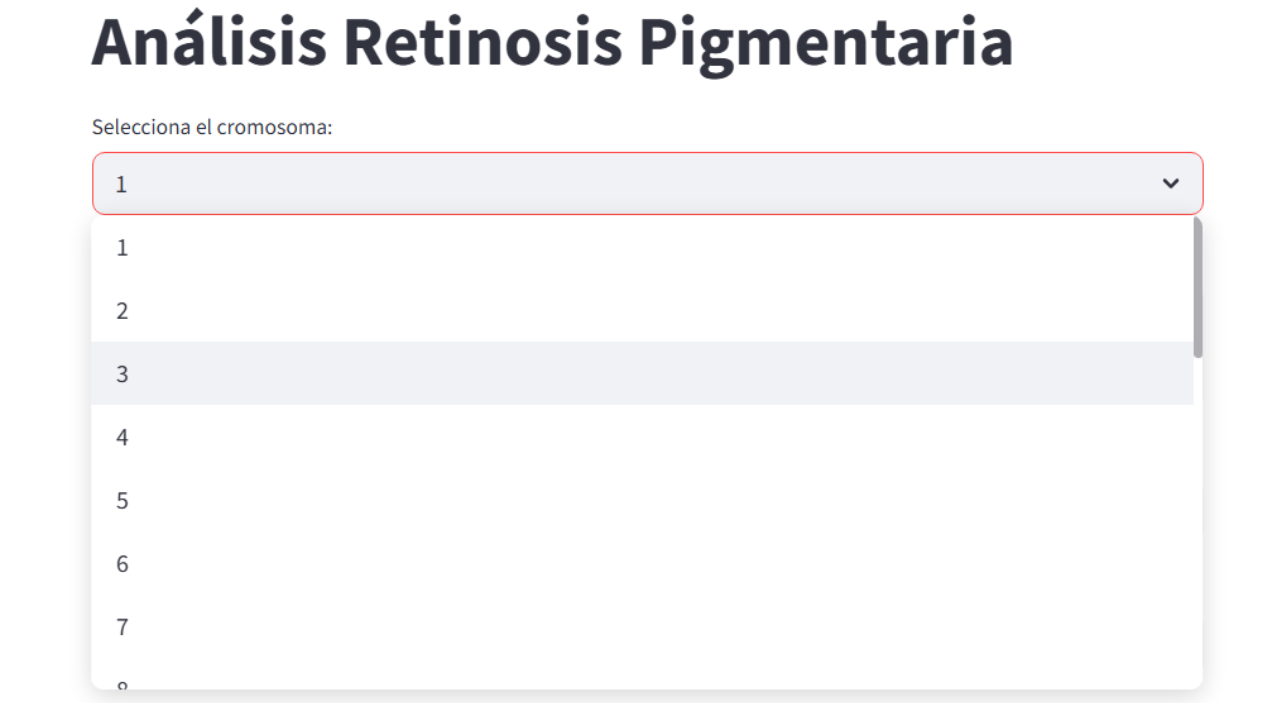
\includegraphics[width=0.9\textwidth]{cromosoma_RP.png}
      \caption{Menú desplegable de selección de cromosoma en la interfaz de usuario.}
      \label{fig:etiqueta_opcional6}
   \end{figure}
   \item Se debe proporcionar un archivo con las mutaciones del paciente en formato \acs{VCF}, cargado a través de subida de archivos. 
   \begin{figure}[H]
      \centering
      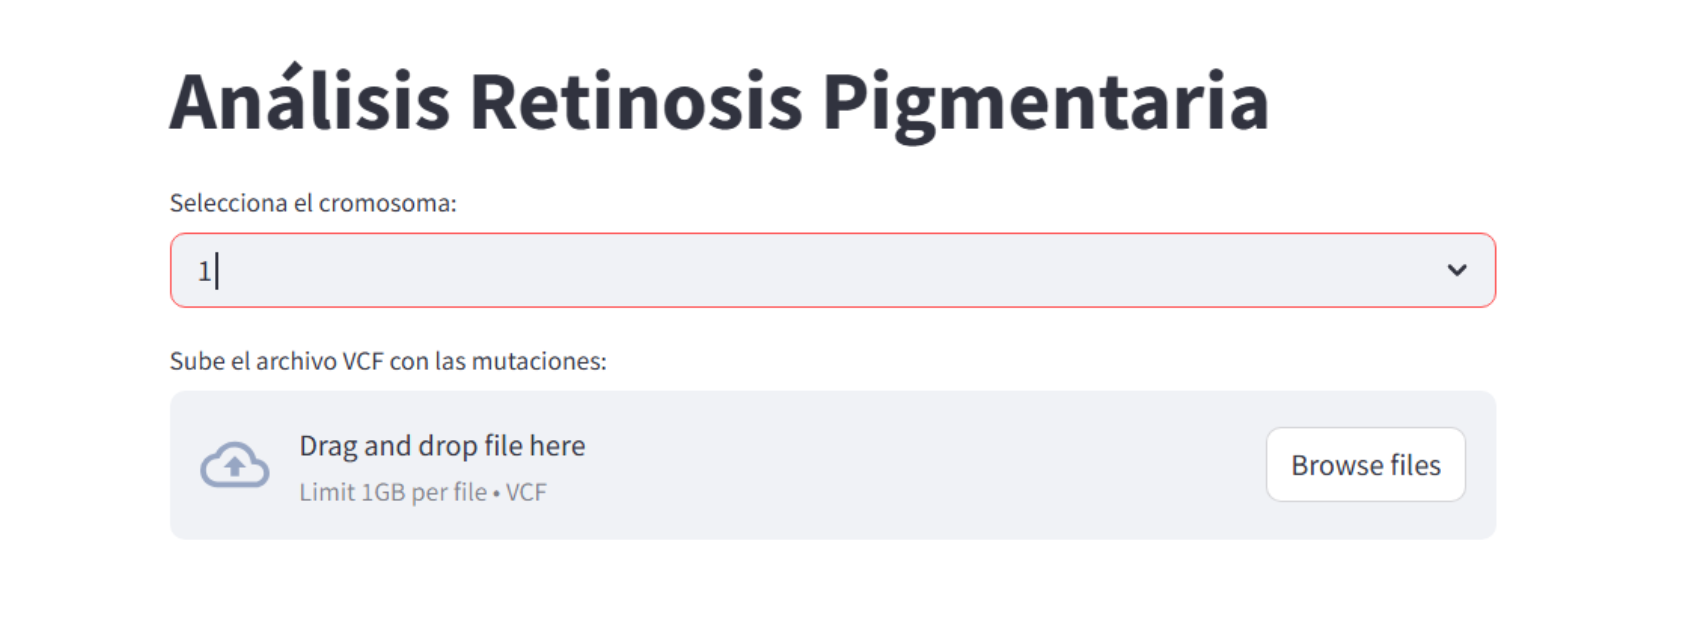
\includegraphics[width=0.9\textwidth]{VCF_RP.png}
      \caption{Buscador de archivos en el sistema para proporcionar \acs{VCF} en la interfaz de usuario.}
      \label{fig:etiqueta_opcional7}
   \end{figure}
   \item Tamaño de k-mer ($k$), que define el tamaño de las secuencias. 
   \item Orden del modelo de Markov ($k_{\text{markov}}$), que determina cuántos símbolos anteriores se consideran en la probabilidad condicional.
   \item Tamaño de ventana para densidad ($l$), que establece el rango en el que se tienen en cuenta las mutaciones alrededor de cada variante. 
   \item Tamaño de ventana para entropía ($w$), para el cálculo de las entropías.
   \item Posición de inicio y tamaño del bloque, para definir el segmento del cromosoma a analizar y así no cargar regiones genómicas excesivamente grandes. 
\end{itemize}

\begin{figure}[H]
      \centering
      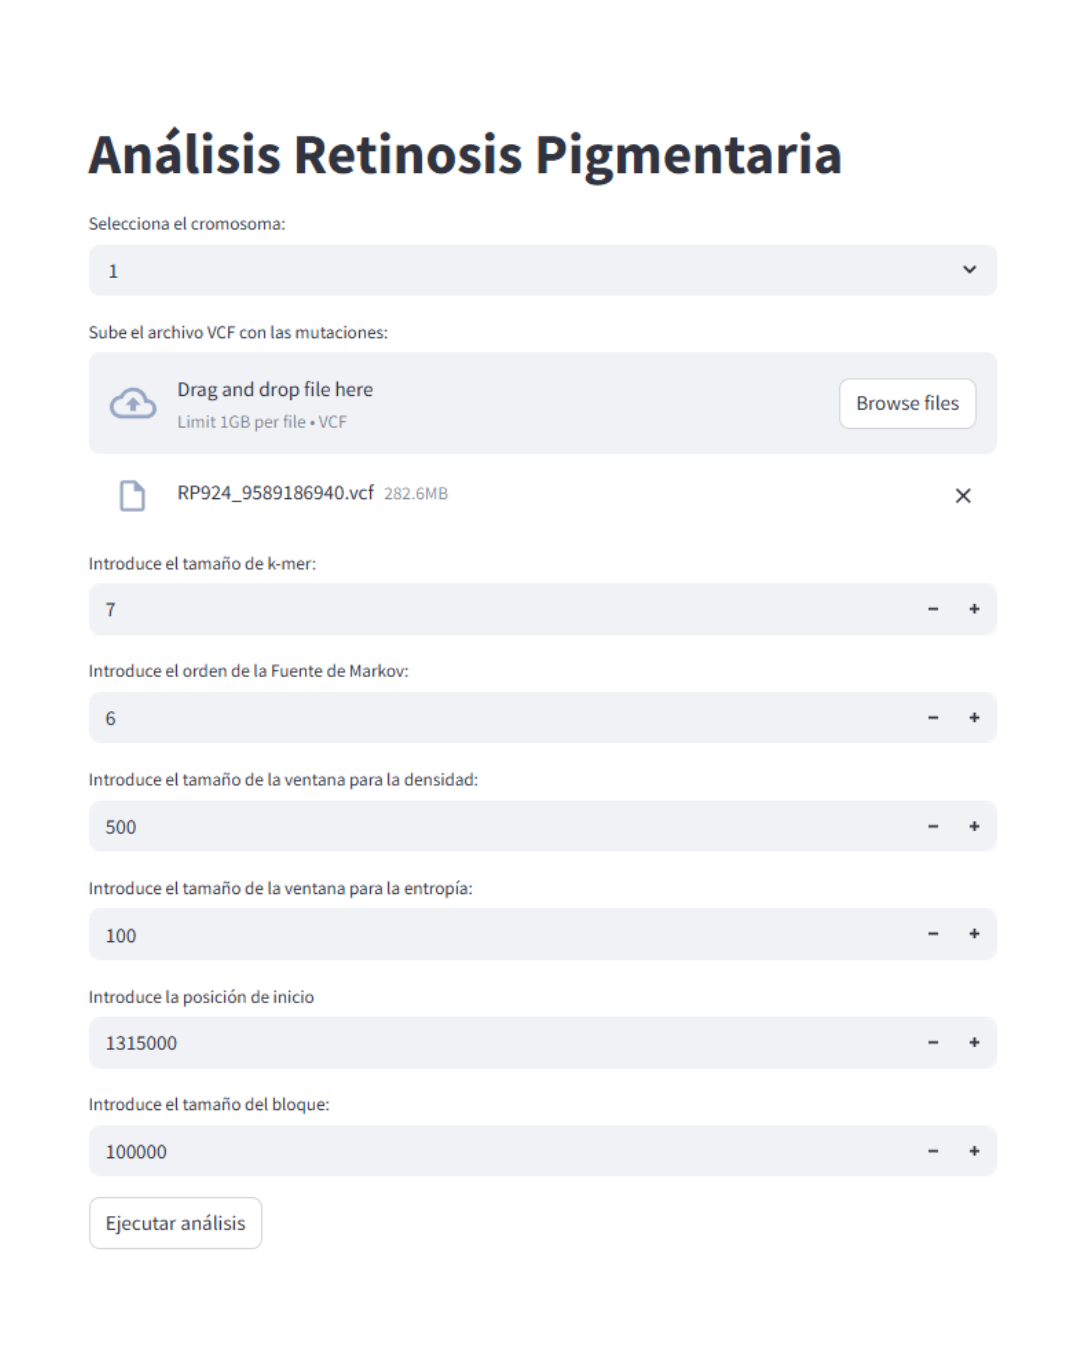
\includegraphics[width=0.9\textwidth]{Analisis_RP.png}
      \caption{Parámetros configurables para el análisis en la interfaz de usuario.}
      \label{fig:etiqueta_opcional8}
   \end{figure}
 

Una vez introducidos estos datos, la aplicación se encarga de ejecutar la lógica del programa: aplica las mutaciones del archivo \acs{VCF} sobre la secuencia original, calcula la entropía simple y la entropía basada en probabilidades condicionales, analiza la densidad de mutaciones en regiones del genoma y genera los gráficos y archivos correspondientes. Finalizado este análisis, se devuelven las siguientes salidas:  

\begin{itemize}
   \item Tres imágenes descargables con los gráficos de entropía simple, entropía condicional (o de Markov) y densidad de mutaciones. 
   \begin{figure}[H]
      \centering
      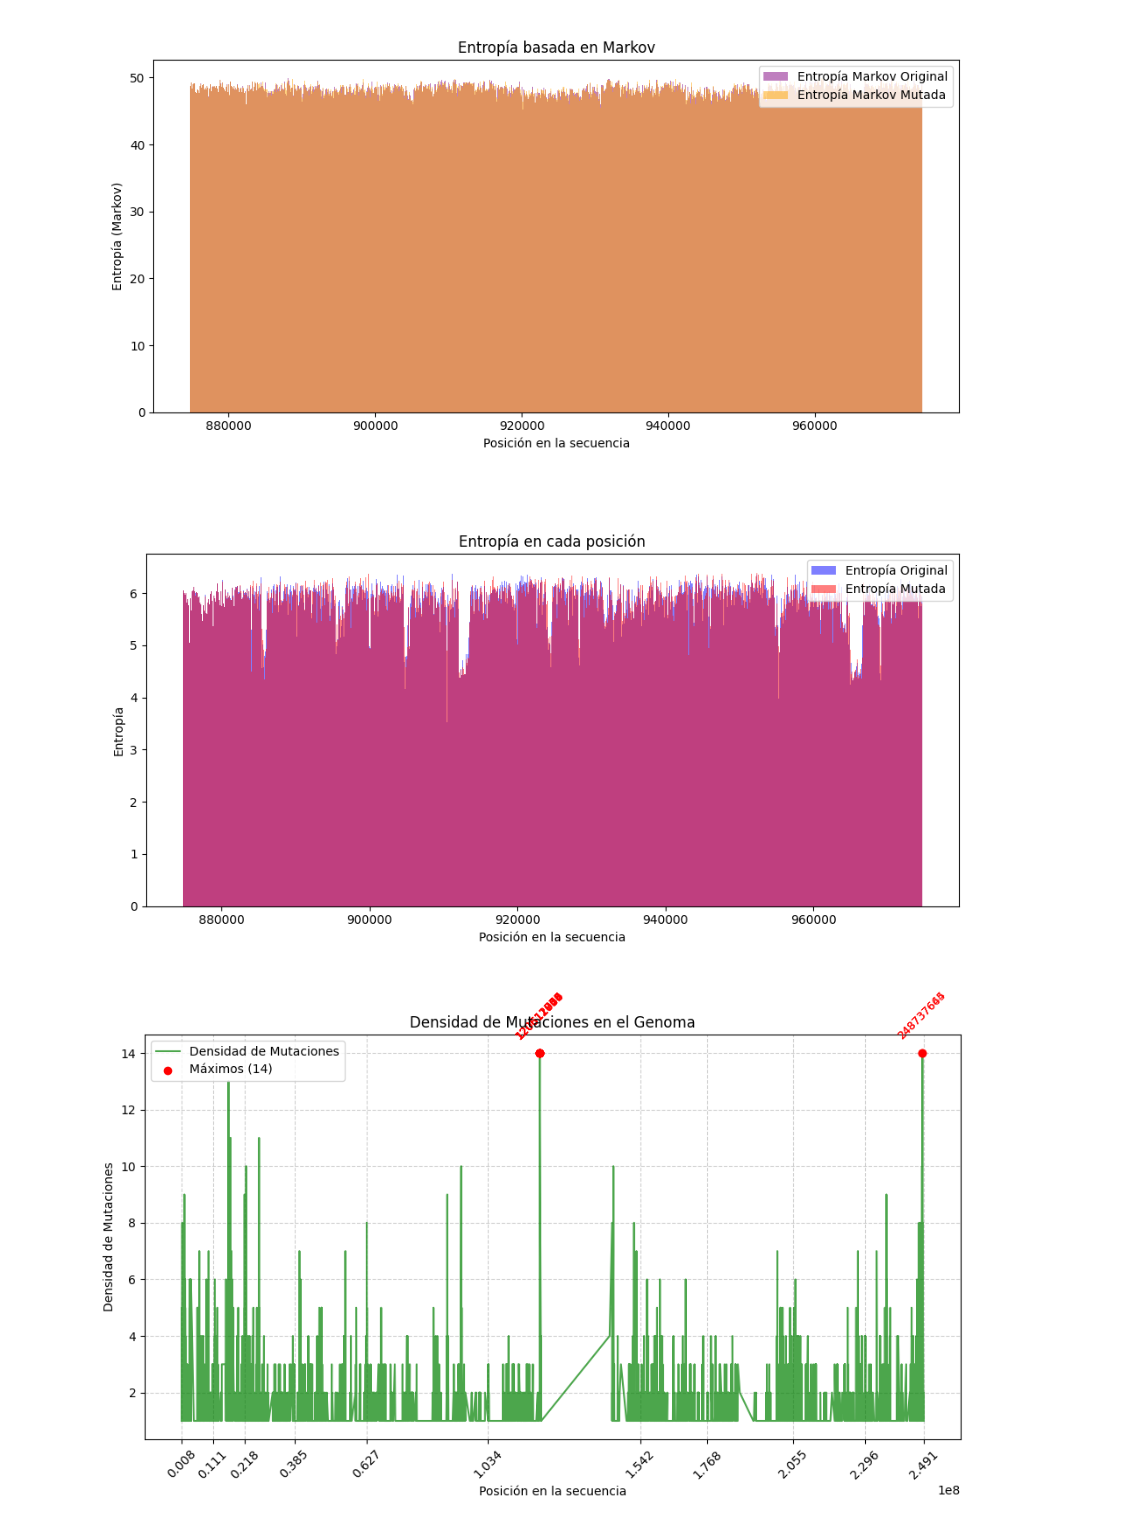
\includegraphics[width=0.9\textwidth]{Graficos_RP.png}
      \caption{Imágenes de los gráficos resultantes del análisis en la interfaz de usuario.}
      \label{fig:etiqueta_opcional9}
   \end{figure}
   \item Tres archivos para descargar: dos ficheros de texto con las fuentes de Markov de la secuencia original y secuencia mutada (los generados a partir de fuentes de Markov), y un archivo con las mutaciones que no han podido aplicarse. 
   \begin{figure}[H]
      \centering
      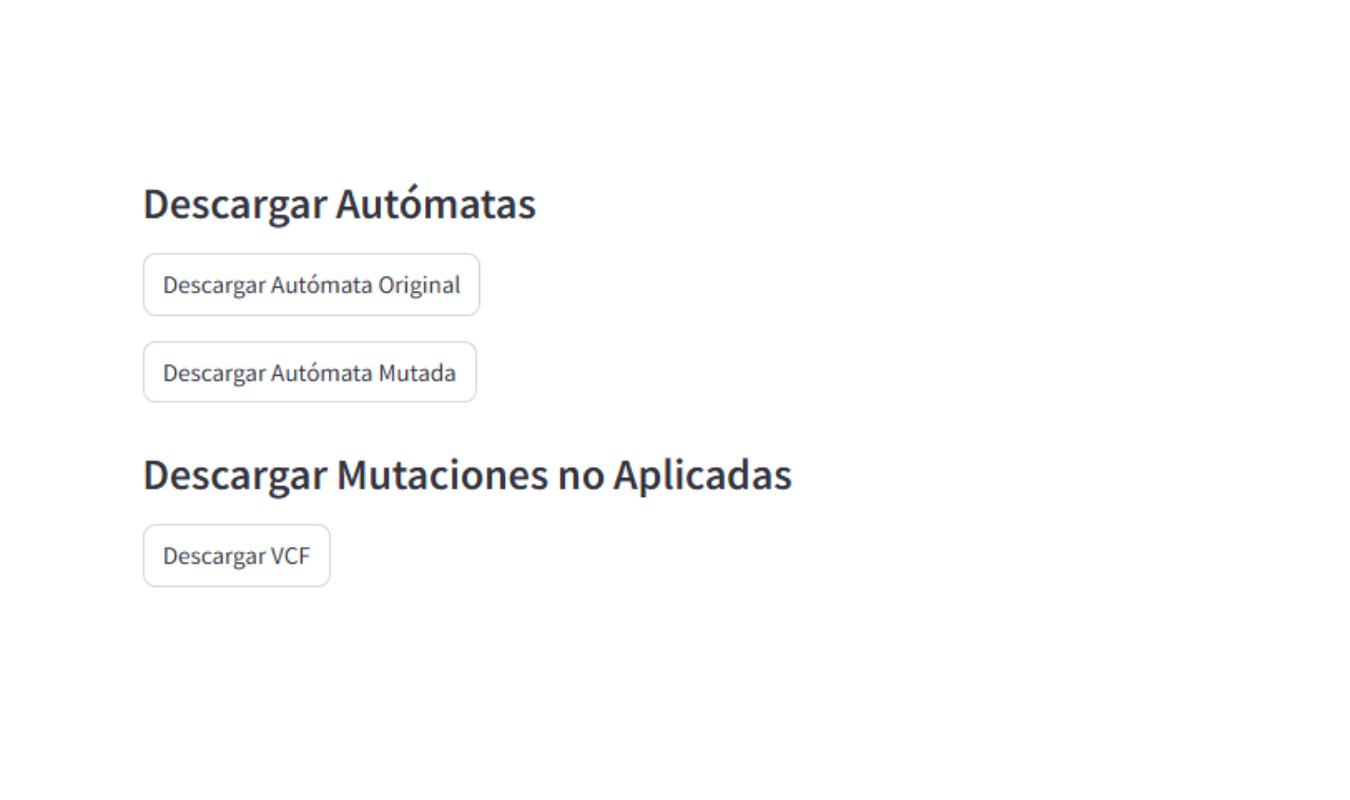
\includegraphics[width=0.9\textwidth]{Automatas_RP.png}
      \caption{Archivos para descargar con las fuentes de Markov resultantes del análisis en la interfaz de usuario.}
      \label{fig:etiqueta_opcional10}
   \end{figure}
   \item Además, se proporciona la opción de descargar un archivo comprimido (.zip) que incluye todos los resultados para facilitar su almacenamiento o distribución. 
   \begin{figure}[H]
      \centering
      
\includegraphics[width=0.9\textwidth]{Zip_RP.png}
      \caption{Archivo comprimido para descargar con todos los archivos resultantes del análisis en la interfaz de usuario.}
      \label{fig:etiqueta_opcional11}
   \end{figure}
\end{itemize}
 



\chapter{Experimentos}

Con el objetivo de evaluar la eficacia de este proyecto en la identificación de mutaciones relevantes asociadas a la retinosis pigmentaria, se han diseñado y ejecutado una serie de experimentos sobre datos genómicos para comprobar el comportamiento del sistema desarrollado en distintos escenarios y medir su capacidad para detectar patrones genéticos relevantes mediante técnicas basadas en Teoría de la Información y fuentes de Markov.  

En esta sección se detallan los archivos usados, los valores de los parámetros seleccionados, los procedimientos implementados y los resultados obtenidos, proporcionando un análisis crítico de los mismos. Todo ello con el fin de demostrar la aplicabilidad del enfoque y su correcto funcionamiento en el diagnóstico y estudio del genoma.  

\section{Experimento base}

Para el primer experimento, se trabajará con el cromosoma 1, descargado previamente desde el \acs{NCBI}, y un tamaño de k-mer pequeño para una exploración general del genoma, detección de zonas con variabilidad o entropía anómala. Como consecuencia, tambien debemos trabajar con un valor pequeño para el orden de la Fuente de Markov, ya que este debe ser menor al tamaño de k-mer por la naturaleza de la aplicación. Para ello se seleccionarán los siguientes valores:


\begin{itemize}
   \item Número de cromosoma: 1.
   \item Archivo con las mutaciones: \texttt{RP924\_9589186940.vcf}  (es el archivo \acs{VCF} con las mutaciones proporcionado por \acs{IIS} la Fe).
   \item Tamaño de k-mer: 4.
   \item Orden de la fuente de Markov: 3.
   \item Tamaño de ventana para la densidad: 500.
   \item Tamaño de ventana para la entropía: 100.
   \item Posición de inicio: 874778.
   \item Tamaño de bloque: 100000 
\end{itemize}
 

Una vez configurados estos parámetros, se procede a ejecutar el análisis, el cual tiene una duración aproximada de 5 minutos. Transcurrido este tiempo, el análisis finaliza y se imprimen por pantalla los siguientes resultados:

A partir de las gráficas obtenidas, se pueden extraer diversas conclusiones relevantes sobre el comportamiento del genoma ante la presencia de mutaciones y la utilidad de las medidas de entropía para su detección.  

\begin{figure}[H]
      \centering
      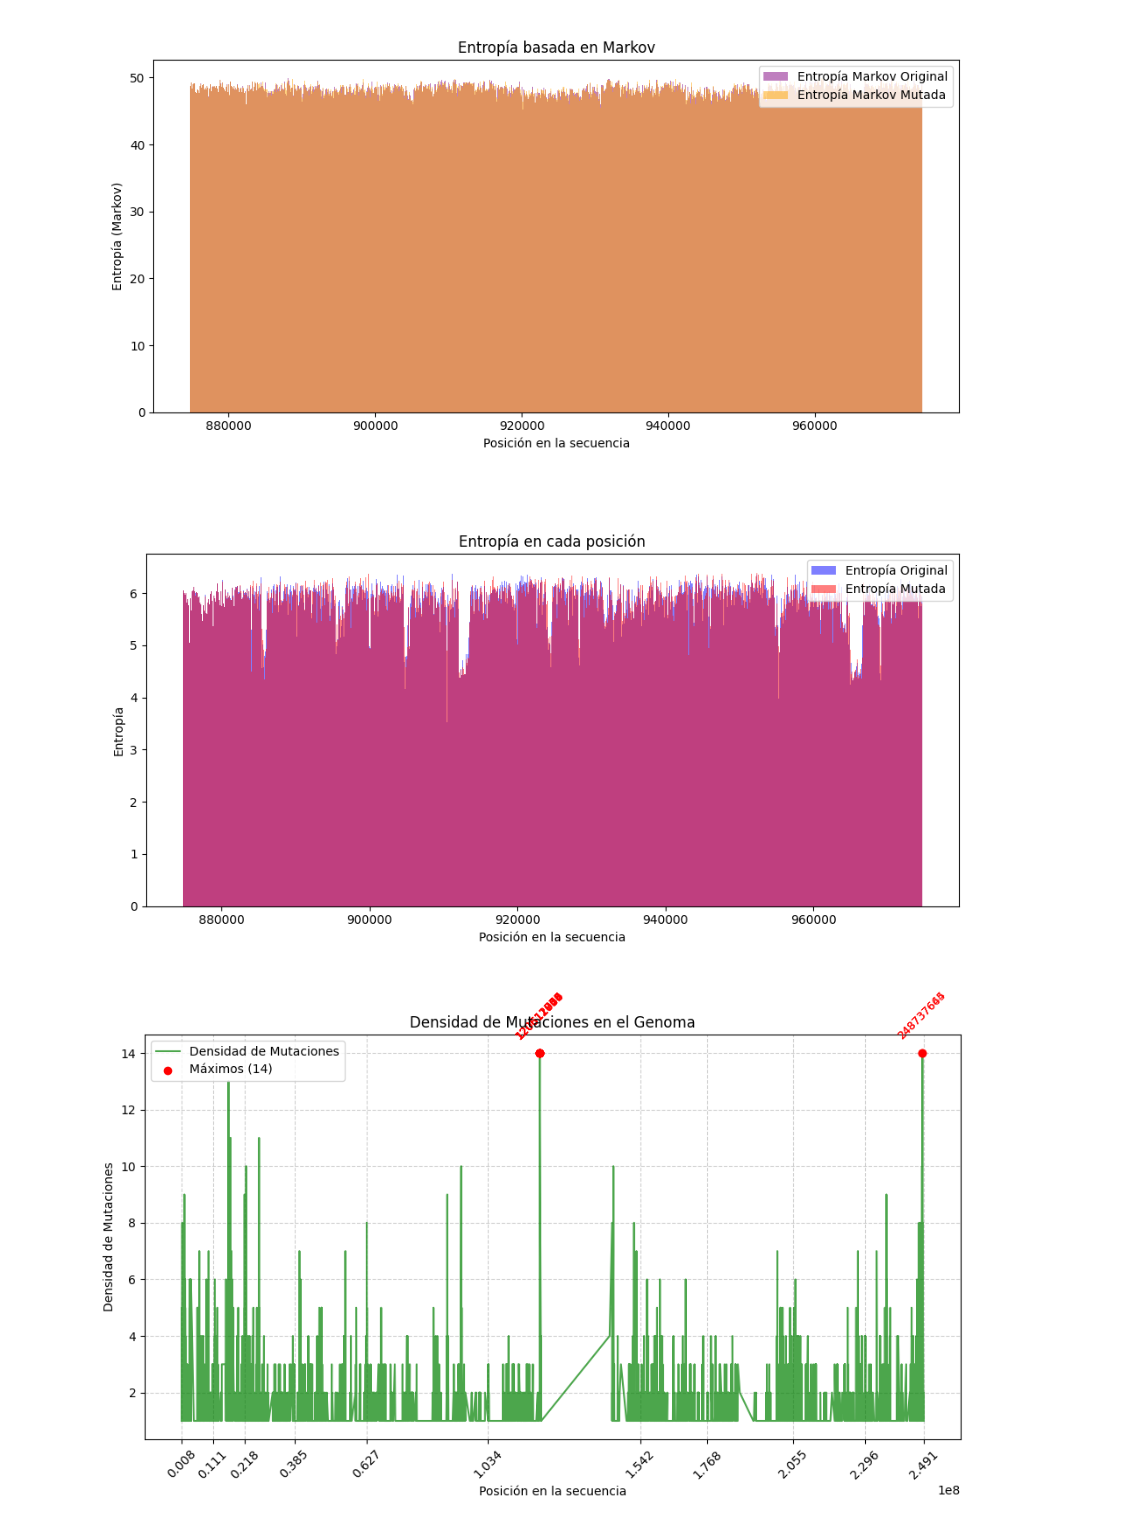
\includegraphics[width=0.9\textwidth]{graf_exp1.png}
      \caption{Gráficas obtenidas a partir del experimento 1.}
      \label{fig:etiqueta_opcional12}
\end{figure}

En la primera gráfica, que representa la entropía simple mediante ventanas deslizantes de tamaño 100 para las secuencias original y mutada, se observan variaciones significativas en los valores de entropía en ciertas regiones. Estas diferencias sugieren que las mutaciones introducidas tienen un impacto en la distribución de los distintos k-mers en esas zonas y, por tanto, permite identificar regiones potencialmente relevantes del genoma. 

La segunda gráfica, que refleja la entropía basada en fuentes de Markov, también mediante ventanas deslizantes de tamaño 100, muestra un comportamiento más similar en ambas versiones de la secuencia, aunque se aprecian pequeñas diferencias en regiones específicas. Esto sugiere que, aunque el modelo de Markov suaviza los valores de entropía, sigue siendo capaz de captar alteraciones y además detectar patrones de mutación que afectan a la dependencia entre símbolos, más allá de su frecuencia individual.  

Finalmente, en la tercera gráfica se representa la densidad de mutaciones a lo largo de la secuencia en ventanas de tamaño 1000 (2x500) centradas en cada mutación. Se identifican varios picos significativos, resaltados en rojo, que indican regiones con alta concentración de mutaciones. Estos máximos podrían coincidir con algunas posiciones en las que se observaron diferencias notables en las medidas de entropía, ya que se podría tratar de regiones del genoma susceptibles de contener variantes genéticas funcionalmente relevantes.  

\begin{figure}[H]
      \centering
      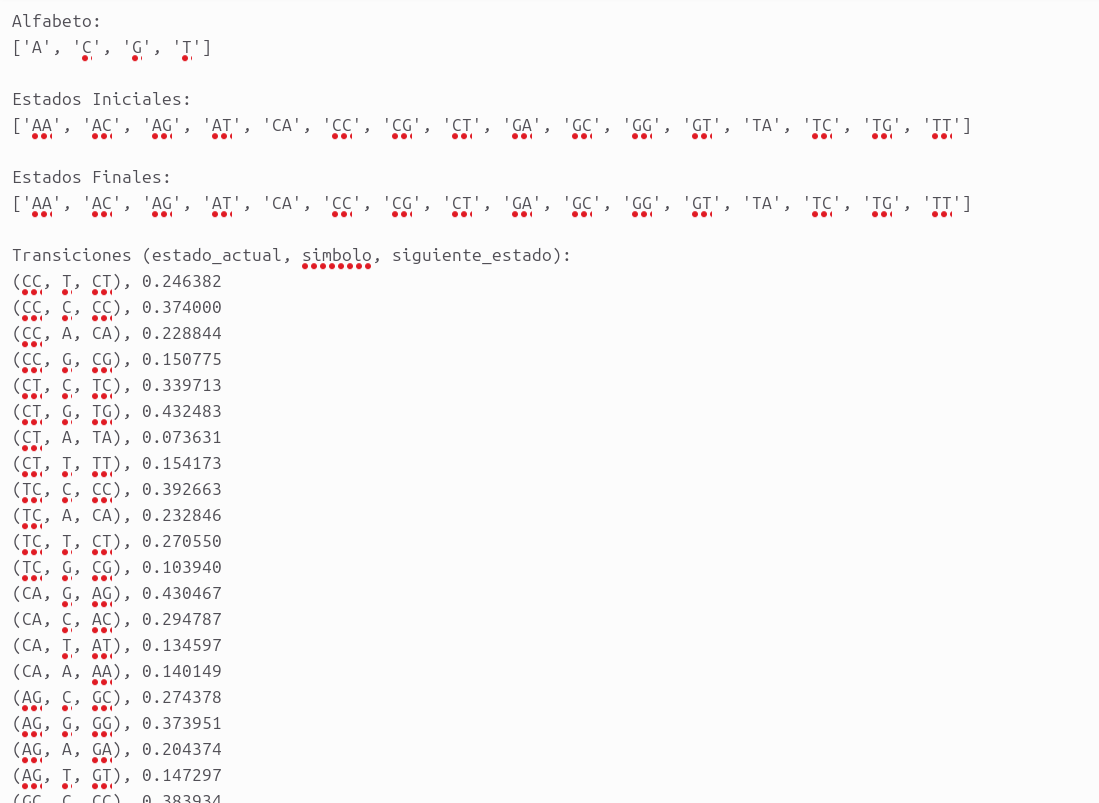
\includegraphics[width=0.8\textwidth]{aut1_exp1.png}
      \caption{Fuente de Markov de la secuencia original obtenido a partir del experimento 1.}
      \label{fig:etiqueta_opcional13}
\end{figure}

\begin{figure}[H]
      \centering
      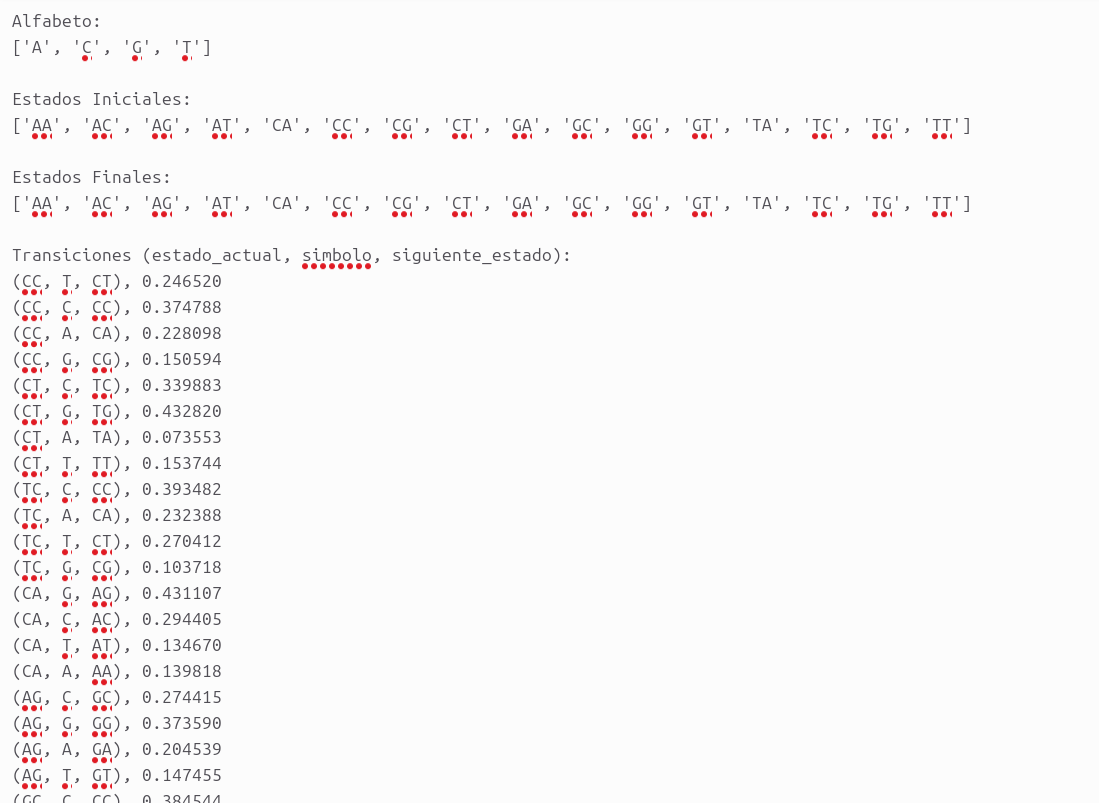
\includegraphics[width=0.8\textwidth]{aut2_exp1.png}
      \caption{Fuente de Markov de la secuencia mutada obtenido a partir del experimento 1.}
      \label{fig:etiqueta_opcional14}
\end{figure}

A partir de los archivos de ambas fuentes de Markov se puede extraer la siguiente información: tanto la fuente con la secuencia original como la mutada comparten el mismo alfabeto y los mismos estados iniciales y finales. Sin embargo, aunque ambos archivos muestran las mismas transiciones, la frecuencia de transición entre estados sí ha cambiado y esto afecta directamente a la entropía condicional basada en el modelo de Markov, ya que las frecuencias de uso de las transiciones pueden generar una distribución de probabilidades diferente, aumentando o disminuyendo la entropía de determinadas regiones. 

\begin{figure}[H]
      \centering
      
\includegraphics[width=0.9\textwidth]{mut_exp1.png}
      \caption{Archivo con mutaciones no aplicadas obtenido a partir del experimento 1.}
      \label{fig:etiqueta_opcional15}
\end{figure}

Finalmente, se ha verificado que el archivo generado con las mutaciones no aplicadas está vacío. Este resultado es un buen indicador, ya que significa que todas las variantes recogidas en el archivo \acs{VCF} han podido integrarse correctamente en la secuencia de referencia descargada desde el \acs{NCBI} y no se han producido conflictos entre las bases de referencia especificadas en el \acs{VCF} y las que figuran en la secuencia genómica. 


\section{Experimento con valores grandes para el tamaño de k-mer}

Para este experimento también se trabajará con el cromosoma 1, pero ahora con un tamaño de k-mer grande. De esta manera, podremos observar sobre la misma secuencia y sin modificar el resto de los parámetros, patrones más específicos, especialmente en regiones con alta densidad de mutaciones. Por lo tanto, se han escogido los siguientes valores:

\begin{itemize}
   \item Número de cromosoma: 1.
   \item Archivo con las mutaciones: \texttt{RP924\_9589186940.vcf}  (es el archivo \acs{VCF} con las mutaciones proporcionado por \acs{IIS} la Fe).
   \item Tamaño de k-mer: 12.
   \item Orden de la fuente de Markov: 3.
   \item Tamaño de ventana para la densidad: 500.
   \item Tamaño de ventana para la entropía: 100.
   \item Posición de inicio: 874778.
   \item Tamaño de bloque: 100000 
\end{itemize}

\begin{figure}[H]
      \centering
      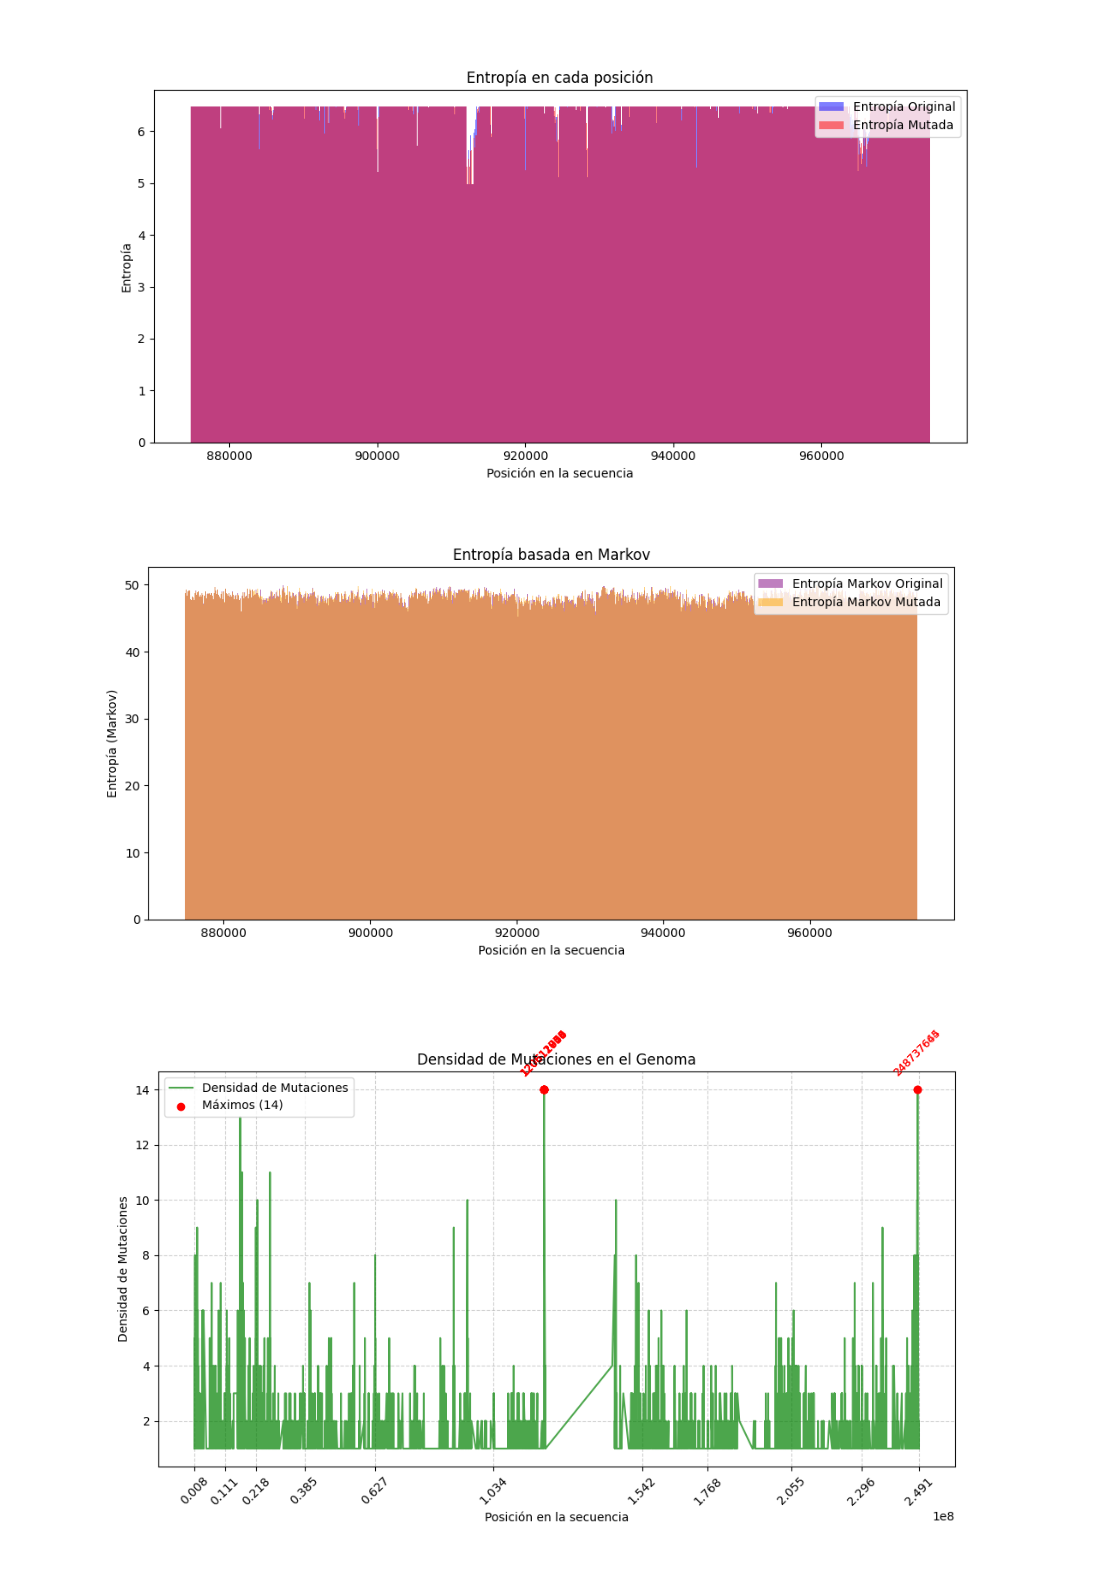
\includegraphics[width=1.0\textwidth]{graf_exp2.png}
      \caption{Gráficas obtenidas a partir del experimento 2.}
      \label{fig:etiqueta_opcional17}
\end{figure}

A la vista de los gráficos, comprobamos que al aumentar el tamaño de k-mer, los valores de entropía en la primera gráfica son notablemente mayores, y además se reduce la variabilidad local. Esto es lógico, ya que un k-mer más largo representa una combinación más específica de bases o nucleótidos, lo que hace que cualquier cambio puntual tenga menos impacto sobre la frecuencia de aparición de todos los posibles k-mers. Por esta razón, se puede deducir que la entropía con k=12 detecta menos ruido. Por otro lado, podemos ver una superposición casi total en la segunda gráfica entre la secuencia original y la mutada, que puede indicar que ahora las mutaciones no afectan de forma significativa las probabilidades de transición. 

Como el aumento del tamaño del k-mer no afecta a la densidad de mutaciones, la tercera gráfica no varía, ya que este análisis se basa únicamente en el recuento local de variantes dentro de ventanas genómicas. 

Por otro lado, las fuentes de Markov generados resultan prácticamente iguales a los del experimento anterior porque el orden de la Fuente de Markov no ha cambiado. La secuencia analizada es la misma, así que no genera una distribución estadística muy distinta con k-mers largos, y la mayoría de las transiciones importantes ya estaban presentes con k=4.

De nuevo, se ha verificado que el archivo generado con las mutaciones no aplicadas está vacío, lo cual es un indicador del buen funcionamiento del programa.


\section{Experimento con valores grandes para el orden de la fuente de Markov}

Esta vez se mantienen todos los parámetros como en el experimento anterior excepto el orden de la fuente de Markov, que aumenta para detectar mutaciones que alteren estructuras locales complejas e identificar zonas funcionales del genoma con mayor precisión. Los valores escogidos son los siguientes:

\begin{itemize}
   \item Número de cromosoma: 1.
   \item Archivo con las mutaciones: \texttt{RP924\_9589186940.vcf}  (es el archivo \acs{VCF} con las mutaciones proporcionado por \acs{IIS} la Fe).
   \item Tamaño de k-mer: 12.
   \item Orden de la fuente de Markov: 7.
   \item Tamaño de ventana para la densidad: 500.
   \item Tamaño de ventana para la entropía: 100.
   \item Posición de inicio: 874778.
   \item Tamaño de bloque: 100000 
\end{itemize}

\begin{figure}[H]
      \centering
      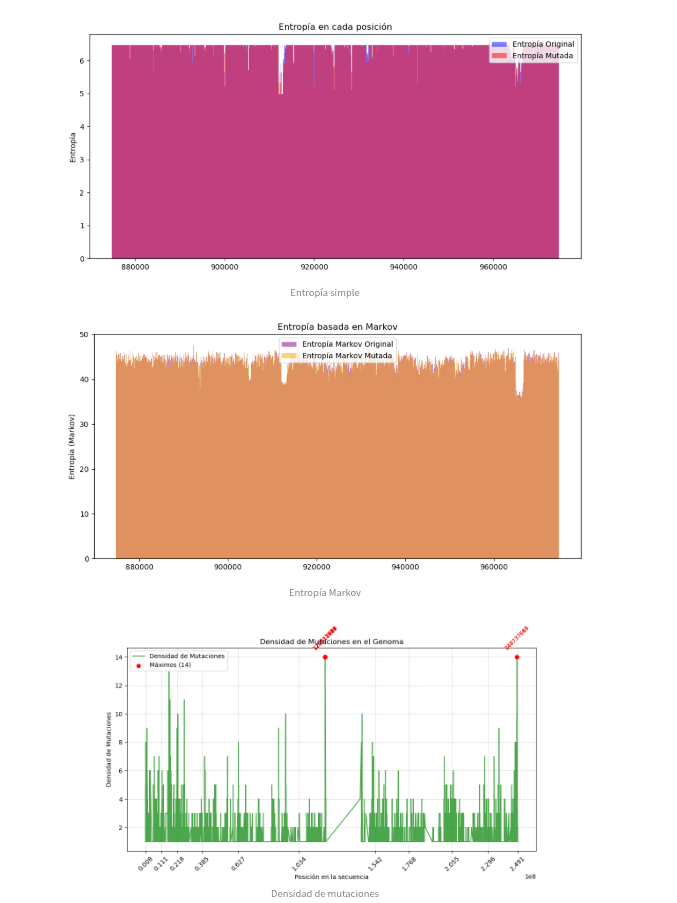
\includegraphics[width=1.0\textwidth]{graf_exp4.png}
      \caption{Gráficas obtenidas a partir del experimento 3.}
      \label{fig:etiqueta_opcional42}
\end{figure}

Tanto en la primera gráfica donde se representa la entropía simple en cada ventana de la secuencia original y la mutada, como en la tercera donde se puede observar la densidad de mutaciones, no se perciben cambios respecto al anterior experimento. Esto es debido a que el parámetro del orden de la fuente de Markov no tiene relación con estas métricas, por lo que sus valores no se modifican.

En cambio, en la segunda gráfica, correspondiente a la entropía basada en fuentes de Markov se nota una mayor separación entre la entropía original y mutada, en comparación con los anteriores experimentos con menor orden de Markov. Además, aparecen picos más definidos de baja entropía, lo que sugiere que el modelo capta regiones con transiciones poco frecuentes, o incluso nuevos estados creados por mutaciones raras.


\begin{figure}[H]
      \centering
      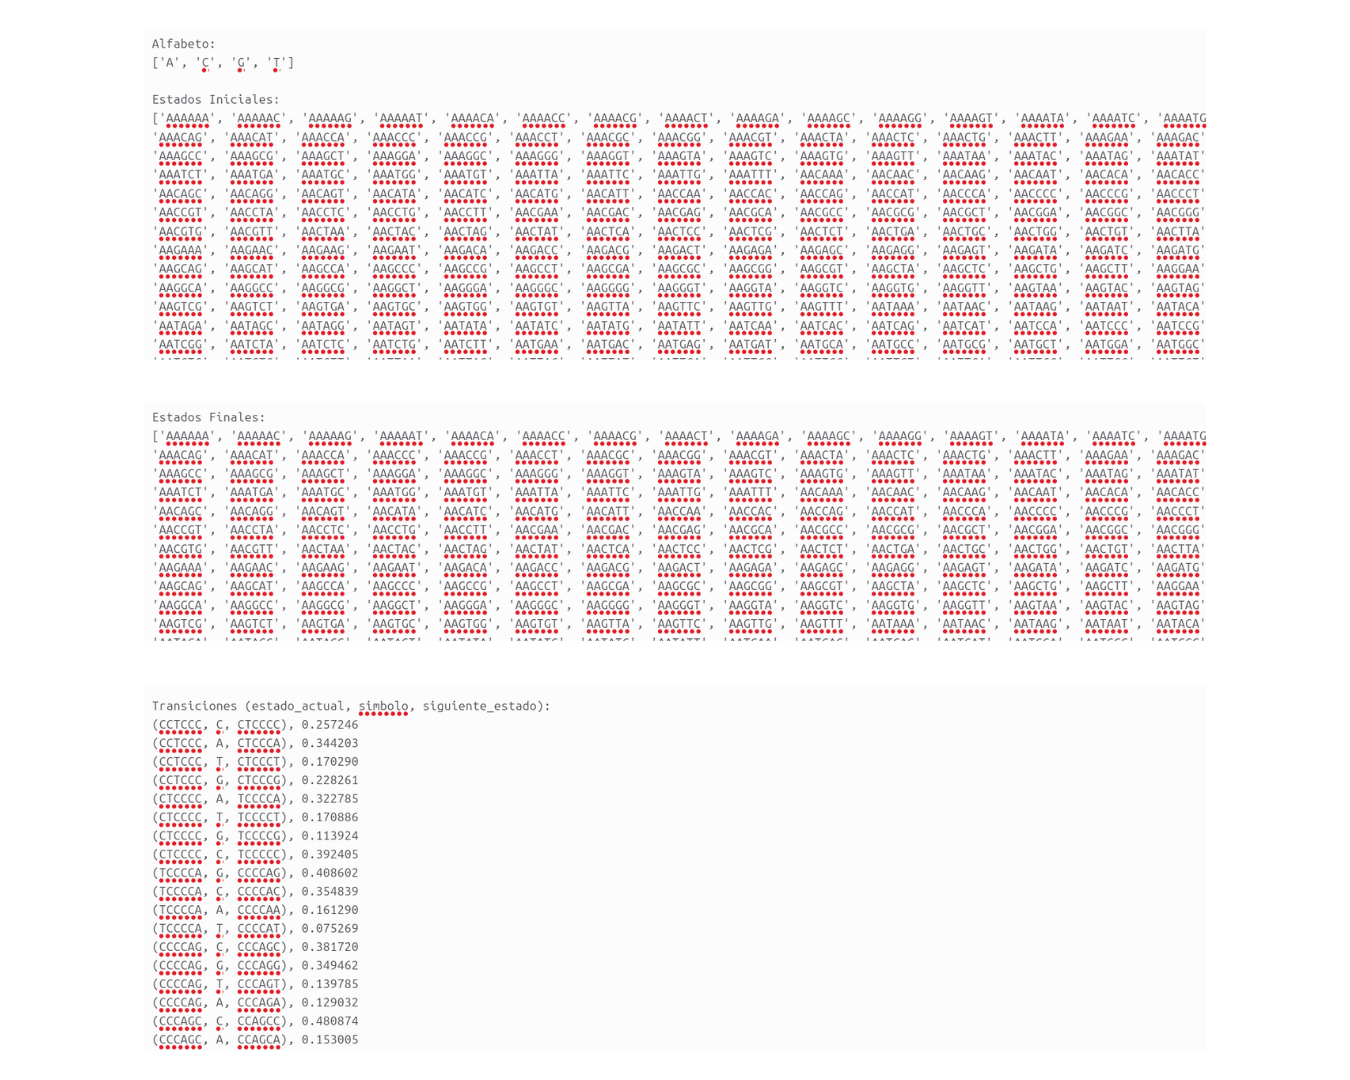
\includegraphics[width=0.8\textwidth]{aut1_exp4.png}
      \caption{Fragmentos de la fuente de Markov de la secuencia original obtenida a partir del experimento 3.}
      \label{fig:etiqueta_opcional43}
\end{figure}

\begin{figure}[H]
      \centering
      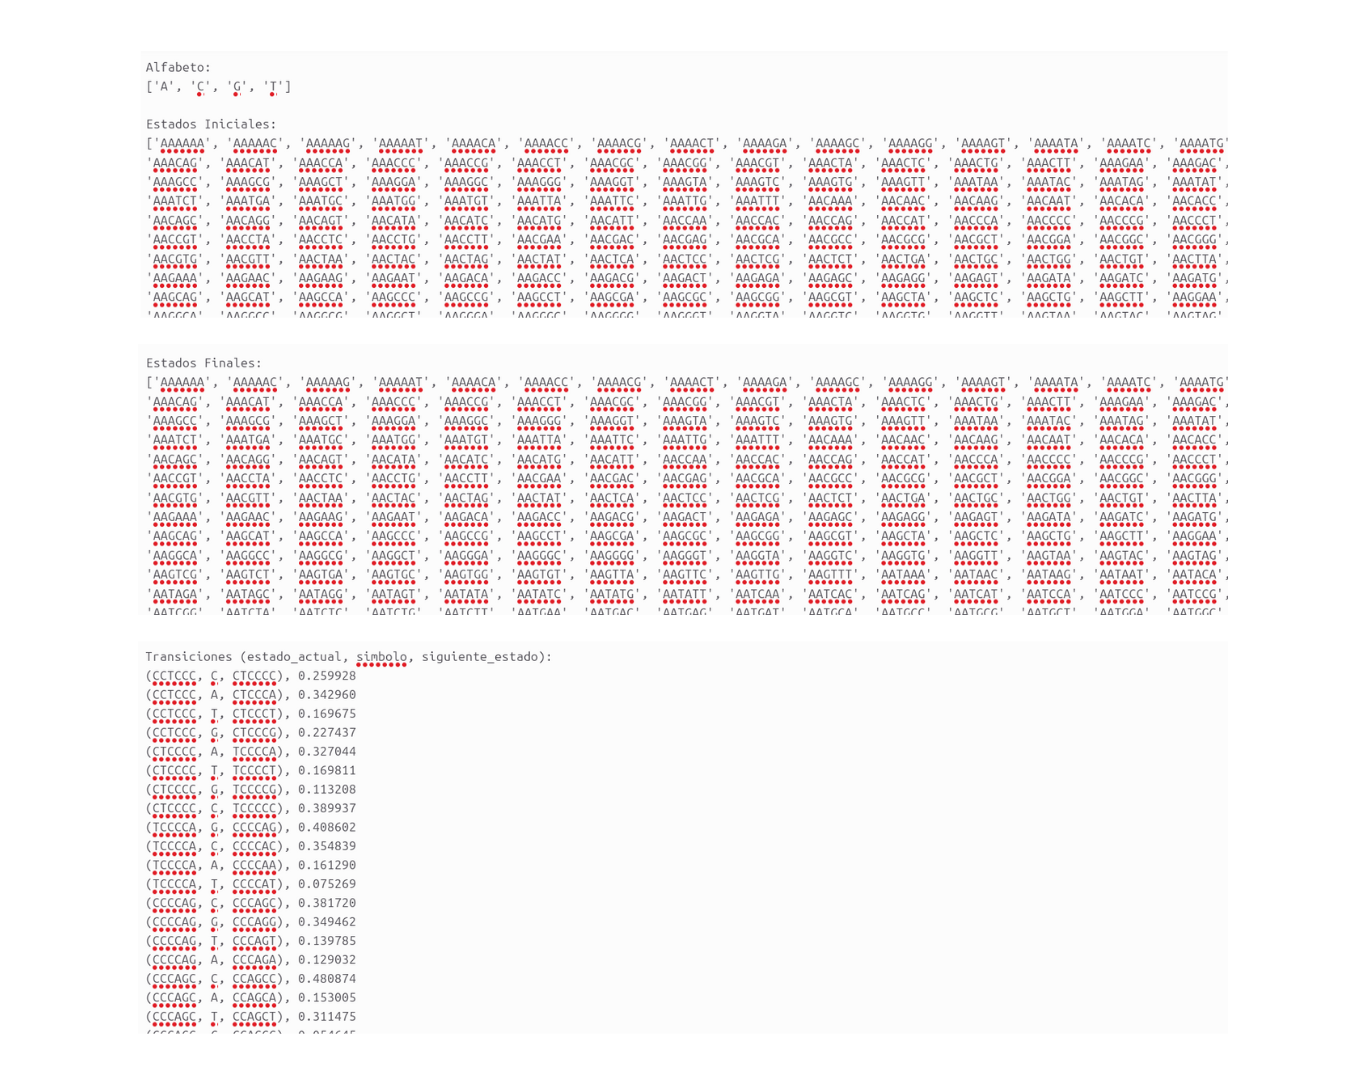
\includegraphics[width=0.8\textwidth]{aut2_exp4.png}
      \caption{Fragmentos de la fuente de Markov de la secuencia mutada obtenida a partir del experimento 3.}
      \label{fig:etiqueta_opcional44}
\end{figure}

Pasando a las fuentes de MArkov generadas, tanto los estados iniciales y finales, como las transiciones ahora estan formados por más nucleótidos. Además, el número de estados y transiciones ha aumentado considerablemente con respecto a las fuentes de Markov generadas anteriormente, ya que al incrementar el orden de la fuente de Markov, los estados pasan a representar combinaciones más largas de nucleótidos. Con un orden mayor, los estados representan contextos más largos y específicos dentro de la secuencia de \acs{ADN}. Esto permite modelar dependencias más complejas entre los nucleótidos.


\section{Experimentos con cromosoma X}

En este experimento se mantienen los parámetros como en el experimento base, pero ahora se explorará el cromosoma X y la posición de inicio pasa a ser 1315000 (comprende una zona con alta proporción de mutaciones), ya que existen genes específicos como el RPGR y el RP2, que están directamente implicados en la retinosis pigmentaria ligada al cromosoma X. Las mutaciones en estos genes son responsables de un porcentaje significativo de los casos de retinosis pigmentaria (\acs{RP}). Por esta razón, se han escogido los siguientes parámetros:

\begin{itemize}
   \item Número de cromosoma: X.
   \item Archivo con las mutaciones: \texttt{RP924\_9589186940.vcf}  (es el archivo \acs{VCF} con las mutaciones proporcionado por \acs{IIS} la Fe).
   \item Tamaño de k-mer: 4.
   \item Orden de la fuente de Markov: 3.
   \item Tamaño de ventana para la densidad: 500.
   \item Tamaño de ventana para la entropía: 100.
   \item Posición de inicio: 1315000.
   \item Tamaño de bloque: 100000 
\end{itemize}

\begin{figure}[H]
      \centering
      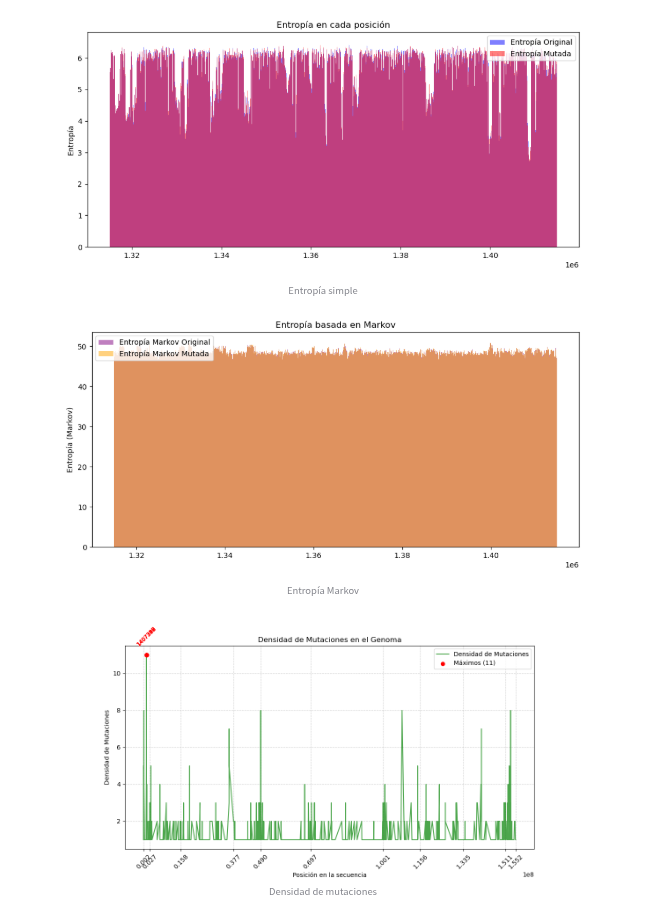
\includegraphics[width=0.9\textwidth]{graf_exp3.png}
      \caption{Gráficas obtenidas a partir del experimento 4.}
      \label{fig:etiqueta_opcional31}
\end{figure}

En la primera gráfica se observa una mayor variabilidad entre la entropía de la secuencia original y la secuencia mutada, en comparación con los experimentos anteriores en el cromosoma 1. Aquí se puede ver que existen regiones localizadas donde se produce una caída significativa de la entropía, lo cual puede indicar regiones funcionales, como genes ligados al sexo. Esto tendría sentido, ya que este se encarga de determinar el sexo en humanos y otros mamíferos, aunque también contiene muchos genes vinculados a enfermedades.

A la vista del segundo gráfico, la entropía Markov se mantiene mucho más constante y elevada, similar a lo observado anteriormente. Sin embargo, también hay ligeras diferencias entre la secuencia original y la mutada, aunque no tan notables como en la entropía simple.

En la gráfica de densidad de mutaciones se observa un máximo claro al principio de la secuencia (marcado con etiqueta roja), pero a lo largo del cromosoma, la densidad se mantiene relativamente baja, lo cual es común en regiones no codificantes o en secuencias menos estudiadas. La posición del máximo, al estar concentrado en una sola región específica del cromosoma, puede reflejar la presencia de genes con alta tasa de variación o de regiones inestables.

Al considerar el modelo de Markov, de nuevo tanto la fuente generada de la secuencia original como la mutada comparten el mismo alfabeto y los mismos estados iniciales y finales. De la misma manera, aunque ambos archivos muestran las mismas transiciones, la frecuencia de transición entre estados sí ha cambiado entre ellos y con respecto al experimento base, aunque sutilmente. Mientras que los gráficos sí reflejan cambios más abruptos en diferentes regiones, la fuente de Markov es más insensible a cambios puntuales, ya que necesita modificaciones significativas en la distribución de transiciones para reflejar una diferencia más pronunciada.

Esta vez también se encuentra vacío el archivo generado con las mutaciones no aplicadas, lo demuestra el buen funcionamiento incluso en diferentes regiones genómicas.\\\\\\

En conjunto, estos resultados demuestran que el análisis computacional de la entropía, tanto clásica como basada en modelos de Markov permite detectar con eficacia alteraciones en el genoma. Esto respalda el potencial del enfoque desarrollado en este proyecto como herramienta de apoyo en el diagnóstico de enfermedades genéticas como la retinosis pigmentaria, contribuyendo al avance en métodos no invasivos y automáticos de análisis genético.

No obstante, es importante destacar que los resultados obtenidos, incluyendo las gráficas y patrones identificados, deben ser ahora revisados y evaluados por expertos en medicina y genómica. Solo profesionales especializados podrán determinar si las diferencias observadas son clínicamente relevantes y validar si pueden utilizarse para el estudio de la \acs{RP}.


%%%%%%%%%%%%%%%%%%%%%%%%%%%%%%%%%%%%%%%%%%%%%%%%%%%%%%%%%%%%%%%%%%%%%%%%%%%%%%%
%                                 CONCLUSIONS                                 %
%%%%%%%%%%%%%%%%%%%%%%%%%%%%%%%%%%%%%%%%%%%%%%%%%%%%%%%%%%%%%%%%%%%%%%%%%%%%%%%

\chapter{Conclusiones}

El presente Trabajo de Fin de Grado ha explorado el uso de herramientas basadas en la Teoría de la Información y modelos de fuentes de Markov para analizar secuencias genómicas asociadas a la \acs{RP}. A partir de secuencias de referencia obtenidas del \acs{NCBI} y mutaciones extraídas de archivos \acs{VCF} proporcionados por el \acs{IIS} La Fe, se ha construido una herramienta capaz de detectar regiones genómicas con alta variabilidad o con alteraciones inusuales.

Uno de los objetivos principales ha sido garantizar una correcta integración de las variantes sobre la secuencia de referencia. Para ello, se han empleado herramientas bioinformáticas como Biopython y vcfpy que permiten trabajar con los formatos de los archivos proporcionados. La correcta aplicación de las mutaciones sobre la secuencia de referencia se ha validado al observar que, en las ejecuciones realizadas en la sección de experimentos, el archivo de mutaciones no aplicadas resultó vacío, lo que indica que no se han producido conflictos entre los datos. Esto da fiabilidad al análisis y refuerza el potencial del sistema para ser usado con datos clínicos reales.

Sobre la secuencia mutada y la original, se han aplicado diferentes enfoques de análisis complementarios. En primer lugar, se ha calculado la entropía en ventanas deslizantes a lo largo de la secuencia para detectar variaciones estadísticas que indiquen cambios en la distribución de los nucleótidos, lo cual podría estar relacionado con regiones funcionales o mutaciones relevantes. Posteriormente, se ha utilizado un modelo de fuente de Markov de orden k para construir una fuente de Markov que representa las probabilidades de transición entre distintos estados definidos por k-mers, permitiendo así un análisis más profundo de la estructura secuencial del \acs{ADN}. Además, se ha incorporado un análisis de densidad de mutaciones mediante el uso de ventanas centradas en cada variante, con el objetivo de localizar zonas con una alta concentración de mutaciones en el genoma.

Con el fin de facilitar el uso de esta herramienta a usuarios que no poseen conocimientos avanzados en programación o informática, se ha desarrollado una interfaz gráfica utilizando la librería Streamlit. Esta interfaz permite cargar los archivos genómicos, ajustar los parámetros del análisis (como el tamaño de los k-mers, el orden de Markov o el tamaño de las ventanas), ejecutar el análisis completo, y visualizar los resultados en forma de gráficos. Además, ofrece la posibilidad de descargar los archivos resultantes (como las fuentes de Markov generadas o los informes de mutaciones no aplicadas) para su posterior estudio. Esta capa de abstracción permite que investigadores biomédicos, técnicos de laboratorio o personal sanitario puedan utilizar la herramienta sin necesidad de interactuar directamente con el código, lo que representa un paso importante hacia la usabilidad en contextos clínicos reales.

\section{Trabajo futuro}

Aunque los resultados obtenidos pueden ser prometedores, el presente trabajo puede ampliarse y mejorarse en distintas direcciones:

\subsection{Ampliación a otras enfermedades raras}

Un trabajo futuro que podría ser prometedor consiste en extender el sistema desarrollado al estudio de otras enfermedades raras causadas por mutaciones genéticas, más allá de la \acs{RP}. Dado que muchas enfermedades raras comparten características con la \acs{RP}, como la elevada heterogeneidad genética, la escasez de datos anotados, y la dificultad diagnóstica por culpa del volumen de variantes generadas por tecnologías de secuenciación. Por esta razón resulta razonable pensar que este proyecto podría ser útil también en otros contextos.

Además, aplicar esta herramienta a otras enfermedades, como la de Charcot-Marie-Tooth (afección hereditaria que afecta los nervios periféricos, causando debilidad muscular, pérdida de sensación y deformidades en los pies y manos\cite{MEDL}), permitiría verificar su validez y capacidad de generalización, como por ejemplo enfermedades raras neuromusculares, metabólicas o del desarrollo que también requieren métodos para reducir el espacio de búsqueda.

Por último, este enfoque también permitiría comparar cómo es la información en las diferentes enfermedades y explorar si ciertas regiones genómicas muestran patrones similares de entropía o transiciones anómalas en distintas patologías, lo cual podría abrir nuevas vías para encontrar regiones funcionales compartidas o mecanismos genómicos comunes.

\subsection{Aplicación de técnicas de Machine Learning}

Otra posible mejora del sistema desarrollado sería la incorporación de algoritmos de Machine Learning (\acs{ML}) o metaheurísticas para lograr optimizar de manera automática los valores de parámetros principales utilizados en los análisis. Actualmente algunos valores como el tamaño de los k-mers, el orden de la fuente de Markov o el tamaño de las ventanas se configuran manualmente, y como hemos visto en la sección anterior, influyen de forma significativa en la sensibilidad y especificidad del modelo para detectar patrones relevantes en la secuencia genómica.

De esta manera, mediante el uso de técnicas de aprendizaje automático, como métodos de validación cruzada (cross-validation), el sistema podría evaluar diferentes combinaciones de parámetros y seleccionar aquellas que maximicen diferentes criterios, como podría ser la identificación de regiones con mutaciones significativas y regiones neutras, o la concordancia con anotaciones clínicas existentes. Este enfoque permitiría adaptar dinámicamente el análisis a distintos genes, regiones genómicas o tipos de enfermedades, sin requerir la intervención manual del usuario.

Aunque actualmente solo se dispone de una pequeña cantidad de diagnósticos para la \acs{RP}, se podrían emplear modelos de ML supervisado donde las variantes genéticas hayan sido clasificadas como patogénicas o benignas por expertos. Estos modelos podrían aprender representaciones complejas del genoma que escapen a métodos estadísticos clásicos. En ese caso se podrían aplicar técnicas como los árboles de decisión, random forests, redes neuronales o boosting para identificar combinaciones de patrones en los perfiles de las entropías y densidad de mutaciones que tengan correlación con la potencial patogenicidad de una variante.


\subsection{Exploración de otras métricas de Teoría de la Información}

Aunque en este proyecto se ha utilizado la entropía como herramienta principal para medir la incertidumbre, se podría plantear el uso de otras métricas del campo de la Teoría de la Información en futuros desarrollos con el objetivo de evaluar si los resultados presentan una mejora con respecto a los previamente obtenidos y si los valores permiten una identificación más precisa de las regiones asociadas a mutaciones patogénicas.

\begin{itemize}
   \item Divergencia de Kullback-Leibler (KL): es una métrica que se utiliza para comparar dos distribuciones. Sobre este trabajo, se podría aplicar para medir las diferencias entre la secuencia original y la mutada, cuantificando cuánto difieren ambas entre sí\cite{BUH}.
   \item Información mutua: mide la cantidad de información que dos variables aleatorias se proporcionan mutuamente. La ambigüedad sobre Y cuando se desconoce X es H(Y). Si se conoce X, la ambigüedad sobre Y disminuye a \( H(Y \mid X) \). Puede emplearse para medir la dependencia entre posiciones del genoma o entre ventanas adyacentes, lo que podría ayudar a detectar correlaciones estructurales\cite{HUS}.
   \item Capacidad del canal: se refiere a la cantidad máxima de información que puede ser transmitida a través de él de forma confiable. Como experimento, se podría estudiar cuánta información puede transmitir una región del \acs{ADN}, ya que valores altos podrían indicar zonas funcionalmente importantes\cite{BLA}.\\
\end{itemize}

Estas métricas podrían complementar o incluso superar a la entropía en algunos casos, como por ejemplo para comparar distribuciones o medir la cantidad de redundancia en el genoma.\\\\\\

En definitiva, este trabajo ha abordado el reto de la combinación entre Teoría de la Información y análisis genómico, proponiendo una solución automatizada y visual que contribuye a optimizar el estudio de enfermedades genéticas raras, y sienta las bases para la investigación con aplicaciones reales en el diagnóstico de enfermedades raras como la \acs{RP}. A medida que se incorporen nuevas herramientas y se integren con otras metodologías, este enfoque podría evolucionar hacia su uso práctico por parte de profesionales del ámbito de la salud.




%%%%%%%%%%%%%%%%%%%%%%%%%%%%%%%%%%%%%%%%%%%%%%%%%%%%%%%%%%%%%%%%%%%%%%%%%%%%%%%
%                                BIBLIOGRAFIA                                 %
%%%%%%%%%%%%%%%%%%%%%%%%%%%%%%%%%%%%%%%%%%%%%%%%%%%%%%%%%%%%%%%%%%%%%%%%%%%%%%%

\begin{thebibliography}{99}

%%%%%%%%%%%%%%%%%%%%%%%%%%%%%%%%%%%%%%%%%%%%%%%%%%%%%%%%%%%%%%%%%%%%%%%%%%%%%%%
% MODEL D'ARTICLE                                                             %
%%%%%%%%%%%%%%%%%%%%%%%%%%%%%%%%%%%%%%%%%%%%%%%%%%%%%%%%%%%%%%%%%%%%%%%%%%%%%%%


   
%%%%%%%%%%%%%%%%%%%%%%%%%%%%%%%%%%%%%%%%%%%%%%%%%%%%%%%%%%%%%%%%%%%%%%%%%%%%%%%
% MODEL DE LLIBRE                                                             %
%%%%%%%%%%%%%%%%%%%%%%%%%%%%%%%%%%%%%%%%%%%%%%%%%%%%%%%%%%%%%%%%%%%%%%%%%%%%%%%

\bibitem{COV}
   Thomas M. Cover and Joy A. Thomas.  
   \newblock \textit{Elements of Information Theory}.  
   \newblock Wiley-Interscience, segunda edición, 2006.

\bibitem{WAT}
   J.~D.~Watson, T.~A.~Baker, S.~P.~Bell, A.~Gann, M.~Levine i R.~Losick.
   \newblock \textit{Molecular Biology of the Gene}.
   \newblock Pearson Education, 7a edició, 2013.
   
\bibitem{ROB}
   Roberto Togneri y Christopher J. S. deSilva.  
   \newblock \textit{Fundamentals of Information Theory and Coding Design}.  
   \newblock CRC Press, Boca Raton, Florida, 2006.

%%%%%%%%%%%%%%%%%%%%%%%%%%%%%%%%%%%%%%%%%%%%%%%%%%%%%%%%%%%%%%%%%%%%%%%%%%%%%%%
% MODEL D'URL                                                                 %
%%%%%%%%%%%%%%%%%%%%%%%%%%%%%%%%%%%%%%%%%%%%%%%%%%%%%%%%%%%%%%%%%%%%%%%%%%%%%%%

\bibitem{VAN}
   Vaño Ribelles, A.  
   \newblock \textit{Análisis, diseño e implementación de clasificadores genómicos para la detección de distrofias hereditarias de la retina mediante técnicas de machine learning}.  
   \newblock Universitat Politècnica de València, 2022.  
   \newblock Disponible en  
   \url{https://riunet.upv.es/handle/10251/185272}
   \newblock Consultado el 13 de junio de 2025.

\bibitem{MAR}
   Martínez Bravo, L. A.  
   \newblock \textit{Diseño de herramientas basadas en teoría de la información para el análisis de información genómica asociada a enfermedades raras}.  
   \newblock Universitat Politècnica de València, 2024.  
   \newblock Disponible en  
   \url{https://riunet.upv.es/handle/10251/210669}
   \newblock Consultado el 13 de junio de 2025.


\bibitem{NAT}
   National Eye Institute.  
   \newblock Retinitis pigmentaria | National Eye Institute.  
   \newblock Disponible en  
   \url{https://www.nei.nih.gov/espanol/aprenda-sobre-la-salud-ocular/enfermedades-y-afecciones-de-los-ojos/retinitis-pigmentaria}.
   \newblock Consultado el 30 de mayo de 2025.

\bibitem{ENF}
   Roche España.  
   \newblock Enfermedades raras: ¿qué debes saber?  
   \newblock s.f.  
   \newblock Disponible en  
   \url{https://www.roche.es/que-hacemos/areas-terapeuticas/enfermedades-raras/enfermedades-raras-que-debes-saber}.  
   \newblock Consultado el 30 de mayo de 2025.

\bibitem{CON}
   Federación Española de Enfermedades Raras (FEDER).  
   \newblock Conoce más sobre las ER.  
   \newblock s.f.  
   \newblock Disponible en  
   \url{https://www.enfermedades-raras.org/enfermedades-raras/conoce-mas-sobre-er}.  
   \newblock Consultado el 30 de mayo de 2025.


\bibitem{GAR}
   Garrity, J.  
   \newblock Estructura y función de los ojos.  
   \newblock \textit{Manual MSD Versión Para Público General}, 11 de marzo de 2024.  
   \newblock Disponible en: 
   \url{https://www.msdmanuals.com/es/hogar/trastornos-oft%C3%A1lmicos/biolog%C3%ADa-de-los-ojos/estructura-y-funci%C3%B3n-de-los-ojos}.  
   \newblock Consultado el 30 de mayo de 2025.

\bibitem{VIS}
   Revista Estudiantil CEUS (Ciencia Estudiantil Unidad de Salud).  
   \newblock Vista de retinosis pigmentaria.  
   \newblock \textit{Revista Estudiantil CEUS}, s.f.  
   \newblock Disponible en: 
   \url{https://ceus.ucacue.edu.ec/index.php/ceus/article/view/8/5}.  
   \newblock Consultado el 30 de mayo de 2025.

\bibitem{DEL}
   Delgado-Pelayo, S. A.  
   \newblock Retinosis Pigmentaria.  
   \newblock \textit{Revista Médica MD}, vol. 3.4(3), pp. 163--166, 2012.


\bibitem{GIL}
   Gil, G. A., Checa, F. L., Borrego, S., Chaparro-Hernández, P., Rueda, T. R., y Sanchez, J.  
   \newblock Estudio de la variabilidad clínica y la heterogeneidad genética en la retinitis pigmentosa.  
   \newblock Dialnet, 1994.    
   \newblock Disponible en  
   \url{https://dialnet.unirioja.es/servlet/articulo?codigo=6768158}.
   \newblock Consultado el 30 de mayo de 2025.

\bibitem{STO}
   Stone, E. M.  
   \newblock Genetic Testing for Inherited Eye Disease.  
   \newblock \textit{Archives of Ophthalmology}, 125(2):205, 2007.  
   \newblock Disponible en
   \newblock \url{https://doi.org/10.1001/archopht.125.2.205}.
   \newblock Consultado el 30 de mayo de 2025.

\bibitem{HAN}
   Hanany, M., Rivolta, C., \& Sharon, D.  
   \newblock Worldwide carrier frequency and genetic prevalence of autosomal recessive inherited retinal diseases.  
   \newblock \textit{Proceedings of the National Academy of Sciences}, 117(5):2710–2716, 2020.  
   \newblock Disponible en
   \newblock \url{https://doi.org/10.1073/pnas.1913179117}.
   \newblock Consultado el 30 de mayo de 2025.

\bibitem{DEC}
   De Castro Miró, M.  
   \newblock \textit{Diagnóstico genético de las distrofias hereditarias de retina mediante secuenciación masiva de nueva generación (NGS)}.  
   \newblock Tesis doctoral, Universitat de València, 2017.  
   \newblock Repositorio UV.  
   \newblock Disponible en
   \newblock \url{https://roderic.uv.es/handle/10550/61138}.
   \newblock Consultado el 30 de mayo de 2025.

\bibitem{SHE}
   Shen, D., Wu, G., \& Suk, H.
   \newblock Deep Learning in Medical Image Analysis.
   \newblock \textit{Annual Review of Biomedical Engineering}, 19(1), 221--248, 2017.
   \newblock Disponible en
   \newblock \url{https://doi.org/10.1146/annurev-bioeng-071516-044442}
   \newblock Consultado el 30 de mayo de 2025.

\bibitem{VER}
   Verana Health.  
   \newblock Why Real-World Data is Key to Providing Insights Into Retinitis Pigmentosa,  
   emés el 20 de novembre de 2024.  
   \newblock Disponible en  
   \url{https://veranahealth.com/why-real-world-data-is-key-to-providing-insights-into-retinitis-pigmentosa/}.
   \newblock Consultado el 30 de mayo de 2025.

\bibitem{HAR}
   Hartong, D. T., Berson, E. L., \& Dryja, T. P.  
   \newblock Retinitis pigmentosa.  
   \newblock \textit{The Lancet}, vol. 368, núm. 9549, pp. 1795--1809, 2006.  
   \newblock Disponible en  
   \url{https://doi.org/10.1016/s0140-6736(06)69740-7}.
   \newblock Consultado el 30 de mayo de 2025.

\bibitem{FER}
   Ferreira, H., Marta, A., Machado, J., Couto, I., Marques, J. P., Beirão, J. M., \& Cunha, A.  
   \newblock Retinitis Pigmentosa Classification with Deep Learning and Integrated Gradients Analysis.  
   \newblock \textit{Applied Sciences}, vol. 15, núm. 4, art. 2181, 2025.  
   \newblock Disponible en  
   \url{https://doi.org/10.3390/app15042181}.
   \newblock Consultado el 30 de mayo de 2025.

\bibitem{STE}
   Stevenson, S.  
   \newblock How deep learning may play a role in predicting retinitis pigmentosa visual impairment,  
   emés el 14 de març de 2023.  
   \newblock Disponible en  
   \url{https://www.ophthalmologytimes.com/view/how-deep-learning-may-play-a-role-in-predicting-retinitis-pigmentosa-visual-impairment}.
   \newblock Consultado el 30 de mayo de 2025.

\bibitem{ISS}
   Issa, Mohamad et al.  
   \newblock Applications of artificial intelligence to inherited retinal diseases: A systematic review.  
   \newblock \textit{Survey of Ophthalmology}, vol. 70, núm. 2, pp. 255--264.  

\bibitem{SEC}
   Societat Espanyola de Ciències de la Computació i Llenguatges (SECal).  
   \newblock Aplicaciones de la Teoría de la Información en Genómica,  
   sense data.  
   \newblock Disponible en  
   \url{https://www.secal.es}.
   \newblock Consultado el 30 de mayo de 2025.

\bibitem{VOZ}
   N.D.  
   \newblock Un algoritmo encuentra indicios de enfermedades en la parte del ADN que teóricamente no servía para nada,  
   emés el 21 d’abril de 2025.  
   \newblock Disponible en  
   \url{https://media.lavozdegalicia.es/noticia/sociedad/2025/04/21/algoritmo-encuentra-indicios-enfermedades-parte-adnconsidera-inutil/00031745236367256507381.htm}.
   \newblock Consultado el 30 de mayo de 2025.

\bibitem{WAN}
   Wang, Y., Juroch, K., Chen, Y., Ying, G., \& Birch, D. G.  
   \newblock Deep Learning–Facilitated Study of the Rate of Change in Photoreceptor Outer Segment Metrics in RPGR-Related X-Linked Retinitis Pigmentosa.  
   \newblock \textit{Investigative Ophthalmology \& Visual Science}, vol. 64, núm. 14, art. 31, 2023.  
   \newblock Disponible en  
   \url{https://doi.org/10.1167/iovs.64.14.31}.
   \newblock Consultado el 30 de mayo de 2025.

\bibitem{ZON}
   ZonaIT.  
   \newblock Avances en la terapia génica para la retinosis pigmentaria causada por mutaciones en el gen RPGR,  
   sense data.  
   \newblock Disponible en  
   \url{https://biotech-spain.com/es/articles/avances-en-la-terapia-g-nica-para-la-retinosis-pigmentaria-causada-por-mutaciones-en-el-gen-rpgr/}.
   \newblock Consultado el 30 de mayo de 2025.

\bibitem{ZHA}
   F.~Zhang, W.~Gu, M.~E.~Hurles, i J.~R.~Lupski.
   \newblock Copy Number Variation in Human Health, Disease, and Evolution.
   \newblock \textit{Annual Review of Genomics and Human Genetics}, 10(1):451--481, 2009.
   \newblock Disponible en
   \newblock \url{https://doi.org/10.1146/annurev.genom.9.081307.164217}.
   \newblock Consultado el 30 de mayo de 2025.
   
\bibitem{JAV}
   Javier, A.  
   \newblock ¿Qué es el formato FASTA?    
   \newblock Disponible en 
   \newblock \url{https://es.scribd.com/document/540407009/que-es-el-formato-fasta}.
   \newblock Consultado el 30 de mayo de 2025.
 
\bibitem{FAS}
   National Center for Biotechnology Information (NCBI).  
   \newblock FASTA Format for Nucleotide Sequences. 
   \newblock Disponible en 
   \newblock \url{https://www.ncbi.nlm.nih.gov/genbank/fastaformat/}.
   \newblock Consultado el 30 de mayo de 2025.
 
\bibitem{AUT}
   Auton, A., Abecasis, G. R., Altshuler, D. M., Durbin, R. M., Bentley, D. R., Chakravarti, A., Clark, A. G., Donnelly, P., Eichler, E. E., Flicek, P., Gabriel, S. B., Gibbs, R. A., Green, E. D., Hurles, M. E., Knoppers, B. M., Korbel, J. O., Lander, E. S., Lee, C., et al.  
   \newblock A global reference for human genetic variation.  
   \newblock \textit{Nature}, 526(7571), 68–74, 2015.  
   \newblock Disponible en 
   \newblock \url{https://doi.org/10.1038/nature15393}.
   \newblock Consultado el 30 de mayo de 2025.
   
\bibitem{GEN}
   National Human Genome Research Institute (NHGRI).  
   \newblock Introduction to Genomics.  
   \newblock Disponible en  
   \newblock \url{https://www.genome.gov/About-Genomics/Introduction-to-Genomics}.
   \newblock Consultado el 30 de mayo de 2025.


\bibitem{EMB}
   EMBL-EBI.  
   \newblock Understanding VCF format | Human genetic variation.  
   \newblock Disponible en 
   \newblock \url{https://www-ebi-ac-uk.translate.goog/training/online/courses/human-genetic-variation-introduction/variant-identification-and-analysis/understanding-vcf-format/?_x_tr_sl=en&_x_tr_tl=es&_x_tr_hl=es&_x_tr_pto=sge}.
   \newblock Consultado el 30 de mayo de 2025.
   
\bibitem{DAN}
   Danecek, P., Auton, A., Abecasis, G., Albers, C. A., Banks, E., DePristo, M. A., Handsaker, R. E., Lunter, G., Marth, G. T., Sherry, S. T., McVean, G., \& Durbin, R.  
   \newblock The variant call format and VCFtools.  
   \newblock \textit{Bioinformatics}, 27(15), 2156–2158, 2011.  
   \newblock \url{https://doi.org/10.1093/bioinformatics/btr330}.
   \newblock Consultado el 30 de mayo de 2025.

\bibitem{GEN}
   Genómica computacional.  
   \newblock Formato FASTA.  
   \newblock \textit{Google Sites}, consultado en mayo de 2025.  
   \newblock Disponible en: 
   \newblock \url{https://sites.google.com/site/genomicaciencias/laboratorio/formato-fasta}.
   \newblock Consultado el 30 de mayo de 2025.

\bibitem{RIN}
   J.~L.~Rinn i H.~Y.~Chang.
   \newblock Genome regulation by long noncoding RNAs.
   \newblock \textit{Annual Review of Biochemistry}, 81:145--166, 2012.
   \newblock Disponible en:
   \newblock \url{https://doi.org/10.1146/annurev-biochem-051410-092902}.
   \newblock Consultado el 30 de mayo de 2025.

\bibitem{MEDL}
   MedlinePlus.  
   \newblock Enfermedad de Charcot-Marie-Tooth: enciclopedia médica.  
   \newblock s.f.  
   \newblock Disponible en  
   \url{https://medlineplus.gov/spanish/ency/article/000727.htm}.  
   \newblock Consultado el 1 de junio de 2025.

\bibitem{BUH}
   Buhl, N.  
   \newblock KL Divergence in Machine Learning.  
   \newblock \textit{Encord}, 4 de noviembre de 2024.  
   \newblock Disponible en  
   \url{https://encord.com/blog/kl-divergence-in-machine-learning/}.  
   \newblock Consultado el 1 de junio de 2025.

\bibitem{HUS}
   Li, H.  
   \newblock Chapter 2 - Basics of communications.  
   \newblock En \textit{Communications for Control in Cyber Physical Systems}, Morgan Kaufmann, 2016, págs. 9--30.  
   \newblock ISBN: 9780128019504.  
   \newblock Disponible en  
   \url{https://www.sciencedirect.com/science/article/pii/B9780128019504000020}.  
   \newblock Consultado el 1 de junio de 2025.

\bibitem{BLA}
   Blahut, R. E.  
   \newblock Information Theory and Coding.  
   \newblock En \textit{Elsevier eBooks}, 2002, págs. 25--31.  
   \newblock Disponible en  
   \url{https://doi.org/10.1016/b978-075067291-7/50027-3}.  
   \newblock Consultado el 1 de junio de 2025.

   

\end{thebibliography}
\cleardoublepage

%%%%%%%%%%%%%%%%%%%%%%%%%%%%%%%%%%%%%%%%%%%%%%%%%%%%%%%%%%%%%%%%%%%%%%%%%%%%%%%
%                           APÈNDIXS  (Si n'hi ha!)                           %
%%%%%%%%%%%%%%%%%%%%%%%%%%%%%%%%%%%%%%%%%%%%%%%%%%%%%%%%%%%%%%%%%%%%%%%%%%%%%%%

\APPENDIX

%%%%%%%%%%%%%%%%%%%%%%%%%%%%%%%%%%%%%%%%%%%%%%%%%%%%%%%%%%%%%%%%%%%%%%%%%%%%%%%
%                                    ODS                                      %
%%%%%%%%%%%%%%%%%%%%%%%%%%%%%%%%%%%%%%%%%%%%%%%%%%%%%%%%%%%%%%%%%%%%%%%%%%%%%%%

\chapter{Objetivos de Desarrollo Sostenible}

\begin{table}[H]
\centering
\caption{Grado de relación del trabajo con los Objetivos de Desarrollo Sostenible (\acs{ODS}).}
\begin{tabular}{|p{7cm}|c|c|c|c|}
\hline
\textbf{Objetivos de Desarrollo Sostenible} & \textbf{Alto} & \textbf{Medio} & \textbf{Bajo} & \textbf{No procede} \\
\hline
ODS 1. Fin de la pobreza. & & & & X \\
ODS 2. Hambre cero. & & & & X \\
ODS 3. Salud y bienestar. & X & & & \\
ODS 4. Educación de calidad. & & & & X \\
ODS 5. Igualdad de género. & & & & X \\
ODS 6. Agua limpia y saneamiento. & & & & X \\
ODS 7. Energía asequible y no contaminante. & & & & X \\
ODS 8. Trabajo decente y crecimiento económico. & & & & X \\
ODS 9. Industria, innovación e infraestructuras. & & X & & \\
ODS 10. Reducción de las desigualdades. & X & & & \\
ODS 11. Ciudades y comunidades sostenibles. & & & X & \\
ODS 12. Producción y consumo responsables. & & X & & \\
ODS 13. Acción por el clima. & & & & X \\
ODS 14. Vida submarina. & & & & X \\
ODS 15. Vida de ecosistemas terrestres. & & & & X \\
ODS 16. Paz, justicia e instituciones sólidas. & & & & X \\
ODS 17. Alianzas para lograr objetivos. & & & & X \\
\hline
\end{tabular}
\end{table}


Este proyecto presenta un alto grado de relación con el Objetivo de Desarrollo Sostenible (\acs{ODS}) 3: Salud y bienestar, ya que se centra en el análisis del genoma humano mediante técnicas de Teoría de la Información con el objetivo de identificar la mutación causante de la \acs{RP}. El diagnóstico temprano y preciso de esta patología permite mejorar la calidad de vida de los pacientes, facilitando un tratamiento adecuado y un mejor seguimiento clínico.

Asimismo, el proyecto se enmarca dentro del ámbito de la investigación científica e innovación tecnológica, lo cual está directamente vinculado con el \acs{ODS} 9: Industria, innovación e infraestructura. La aplicación de métodos computacionales avanzados en el análisis genómico contribuye al desarrollo de nuevas herramientas diagnósticas y promueve el progreso en el campo de la bioinformática y la medicina personalizada.

Además, al estar dirigido al estudio de una enfermedad rara, este trabajo tiene una implicación significativa en la reducción de desigualdades, en concordancia con el \acs{ODS} 10. Las personas afectadas por enfermedades poco frecuentes suelen enfrentar barreras en el acceso al diagnóstico y tratamiento. Este tipo de investigaciones contribuye a reducir esa brecha, promoviendo una atención médica más equitativa y accesible para poblaciones vulnerables.

Finalmente, el uso de herramientas computacionales para la identificación de mutaciones clave en el genoma permite optimizar los recursos utilizados en laboratorios, disminuyendo la necesidad de realizar pruebas físicas extensas. Esto se alinea tanto con el \acs{ODS} 12: Producción y consumo responsables, al fomentar un uso más eficiente de los recursos disponibles, como con el \acs{ODS} 11: Ciudades y comunidades sostenibles, en cuanto a la sostenibilidad de las infraestructuras científicas y sanitarias que prestan estos servicios.



%%%%%%%%%%%%%%%%%%%%%%%%%%%%%%%%%%%%%%%%%%%%%%%%%%%%%%%%%%%%%%%%%%%%%%%%%%%%%%%
%                               ALTRES  APÈNDIXS                              %
%%%%%%%%%%%%%%%%%%%%%%%%%%%%%%%%%%%%%%%%%%%%%%%%%%%%%%%%%%%%%%%%%%%%%%%%%%%%%%%




%%%%%%%%%%%%%%%%%%%%%%%%%%%%%%%%%%%%%%%%%%%%%%%%%%%%%%%%%%%%%%%%%%%%%%%%%%%%%%%
%                              FI DEL DOCUMENT                                %
%%%%%%%%%%%%%%%%%%%%%%%%%%%%%%%%%%%%%%%%%%%%%%%%%%%%%%%%%%%%%%%%%%%%%%%%%%%%%%%

\end{document}
